\section{Structural Estimation results}
\subsection{Barcode-level Elasticities}

\begin{figure}[H]
    \centering
    \caption{Elasticity of substitution $\sigma_p$: Weekly frequency $\sum_{t \in y(t)} \mathbb{1}(P_{il,t}C_{il,t} > 0) \geq 0.5$}
    \label{fig: app_elas_sigma_cats_weekly_50ptt}
    Full sample&i-n-c-y + i-n-c-w + p-n-c-t&68&0.97&0.87&0.03&1.00&0.96&0.01&-1.52&-0.81&-0.25&-3.45&-2.15&-1.12\\
Full sample&i-n-c-y + i-n-c-w + p-n-f-t&68&0.82&0.65&0.16&0.89&0.67&0.26&-1.50&-0.78&-0.25&-5.65&-2.46&0.88\\
Full sample&i-n-c-y + i-n-c-w + p-n-c-f-t&68&0.81&0.65&0.16&0.78&0.66&0.12&-1.24&-0.61&-0.23&-4.94&-2.18&1.04\\ \hdashline
Full sample&i-n-c-y + i-n-c-w + p-r-c-t&68&0.93&0.74&0.03&0.97&0.80&0.01&-1.30&-0.57&-0.20&-3.15&-1.73&-0.97\\
Full sample&i-n-c-y + i-n-c-w + p-r-f-t&68&0.91&0.72&0.04&0.94&0.85&0.02&-1.30&-0.56&-0.21&-3.45&-1.85&-0.72\\
Full sample&i-n-c-y + i-n-c-w + p-r-c-f-t&68&0.94&0.62&0.10&0.99&0.81&0.05&-1.04&-0.45&-0.18&-2.71&-1.58&-0.74\\ \midrule
T $\geq$ 25\%&i-n-c-y + i-n-c-w + p-n-c-t&68&0.87&0.82&0.04&0.95&0.93&0.02&-1.79&-1.05&-0.35&-4.27&-2.87&-1.11\\
T $\geq$ 25\%&i-n-c-y + i-n-c-w + p-n-f-t&68&0.72&0.66&0.15&0.85&0.79&0.12&-1.70&-0.99&-0.34&-6.27&-2.93&1.77\\
T $\geq$ 25\%&i-n-c-y + i-n-c-w + p-n-c-f-t&68&0.72&0.68&0.10&0.87&0.81&0.08&-1.34&-0.75&-0.27&-4.78&-2.79&2.09\\ \hdashline
T $\geq$ 25\%&i-n-c-y + i-n-c-w + p-r-c-t&68&0.91&0.84&0.00&0.96&0.95&0.00&-1.82&-1.05&-0.42&-3.67&-2.52&-0.78\\
T $\geq$ 25\%&i-n-c-y + i-n-c-w + p-r-f-t&68&0.90&0.79&0.03&0.96&0.92&0.01&-1.76&-1.01&-0.44&-3.92&-2.37&-0.44\\
T $\geq$ 25\%&i-n-c-y + i-n-c-w + p-r-c-f-t&68&0.91&0.75&0.04&0.97&0.92&0.01&-1.55&-0.82&-0.33&-3.38&-2.14&-0.39\\ \midrule
T $\geq$ 50\%&i-n-c-y + i-n-c-w + p-n-c-t&68&0.85&0.76&0.04&0.94&0.91&0.02&-2.35&-1.20&-0.22&-5.19&-3.50&0.45\\
T $\geq$ 50\%&i-n-c-y + i-n-c-w + p-n-f-t&68&0.66&0.57&0.12&0.82&0.73&0.09&-2.34&-1.13&-0.28&-7.13&-3.55&0.96\\
T $\geq$ 50\%&i-n-c-y + i-n-c-w + p-n-c-f-t&68&0.69&0.62&0.10&0.82&0.75&0.08&-1.66&-0.89&-0.17&-6.22&-3.22&2.91\\ \hdashline
T $\geq$ 50\%&i-n-c-y + i-n-c-w + p-r-c-t&67&0.90&0.76&0.03&0.96&0.91&0.01&-2.30&-1.32&-0.22&-4.42&-3.10&-0.61\\ 
T $\geq$ 50\%&i-n-c-y + i-n-c-w + p-r-f-t&67&0.82&0.72&0.03&0.94&0.89&0.01&-2.28&-1.21&-0.22&-4.48&-2.70&-0.43\\
T $\geq$ 50\%&i-n-c-y + i-n-c-w + p-r-c-f-t&67&0.84&0.74&0.04&0.95&0.90&0.01&-1.96&-1.02&-0.22&-4.41&-2.56&-0.70\\ \midrule
T $\geq$ 25\% \& M $\geq$ 0.1\%&i-n-c-y + i-n-c-w + p-n-c-t&68&0.85&0.81&0.06&0.94&0.93&0.03&-1.96&-1.13&-0.31&-4.49&-2.98&-0.84\\ 
T $\geq$ 25\% \& M $\geq$ 0.1\%&i-n-c-y + i-n-c-w + p-n-f-t&68&0.72&0.62&0.12&0.83&0.74&0.09&-1.94&-1.05&-0.32&-8.91&-3.12&1.34\\
T $\geq$ 25\% \& M $\geq$ 0.1\%&i-n-c-y + i-n-c-w + p-n-c-f-t&68&0.72&0.63&0.10&0.87&0.77&0.08&-1.58&-0.80&-0.27&-6.09&-2.93&2.19\\ \hdashline
T $\geq$ 25\% \& M $\geq$ 0.1\%&i-n-c-y + i-n-c-w + p-r-c-t&68&0.91&0.82&0.01&0.96&0.95&0.01&-2.00&-1.16&-0.42&-3.90&-2.63&-0.79\\
T $\geq$ 25\% \& M $\geq$ 0.1\%&i-n-c-y + i-n-c-w + p-r-f-t&68&0.88&0.78&0.03&0.96&0.92&0.01&-2.02&-1.12&-0.43&-4.03&-2.50&-0.54\\
T $\geq$ 25\% \& M $\geq$ 0.1\%&i-n-c-y + i-n-c-w + p-r-c-f-t&68&0.91&0.76&0.04&0.97&0.93&0.01&-1.95&-0.92&-0.37&-3.75&-2.21&-0.66\\ \midrule
T $\geq$ 50\% \& M $\geq$ 0.1\%&i-n-c-y + i-n-c-w + p-n-c-t&67&0.84&0.75&0.03&0.94&0.89&0.02&-2.35&-1.20&-0.20&-5.51&-3.50&0.46\\
T $\geq$ 50\% \& M $\geq$ 0.1\%&i-n-c-y + i-n-c-w + p-n-f-t&67&0.60&0.53&0.10&0.74&0.66&0.08&-2.42&-1.15&-0.15&-9.17&-3.64&0.93\\
T $\geq$ 50\% \& M $\geq$ 0.1\%&i-n-c-y + i-n-c-w + p-n-c-f-t&67&0.66&0.59&0.09&0.78&0.71&0.08&-1.84&-0.89&-0.17&-8.27&-3.36&1.22\\ \hdashline
T $\geq$ 50\% \& M $\geq$ 0.1\%&i-n-c-y + i-n-c-w + p-r-c-t&67&0.90&0.76&0.04&0.96&0.91&0.02&-2.47&-1.35&-0.21&-4.55&-3.13&-0.62\\
T $\geq$ 50\% \& M $\geq$ 0.1\%&i-n-c-y + i-n-c-w + p-r-f-t&67&0.84&0.72&0.04&0.94&0.89&0.01&-2.50&-1.28&-0.18&-4.84&-2.81&-0.73\\
T $\geq$ 50\% \& M $\geq$ 0.1\%&i-n-c-y + i-n-c-w + p-r-c-f-t&67&0.85&0.71&0.06&0.95&0.85&0.02&-2.43&-1.05&-0.27&-4.55&-2.59&-0.97\\
\bottomrule

     \parbox{\textwidth}{
        \begin{spacing}{1} 
            {\footnotesize 
            \textit{Notes}: This figure shows the OLS and IV-estimates of the product variety level elasticities of substitution $\sigma_p$ estimated using consumption data at the weekly frequency. The estimations include all product variety-region-week observations for which weekly sales are positive in over 50\% of weeks in a given year. We include product variety-region-chain-year FEs, product variety-region-chain-week and product category-region-chain-week FEs. Alongside the parameters, we plot 95\% confidence intervals based on clustered standard errors at the product variety level. For expositional purposes, we omit estimates for which the confidence intervals are outside of the $[-10,2]$ range.}
        \end{spacing}}
 \end{figure} 

\begin{landscape}
    \begin{table}[H]
        \centering
        \caption{Weekly Barcode-level Elasticities: Within store instrument}
        \label{tab: app_elas_sigma_cats_weekly}
        \begin{spacing}{1}
        \scalebox{0.65}{
        \begin{tabular}{llccccccccccccc} \toprule
            & & &\multicolumn{3}{c}{Unweighted}  &\multicolumn{3}{c}{Weighted} & 
             \multicolumn{3}{c}{OLS} & \multicolumn{3}{c}{IV} \\
             \cmidrule(lr){4-6} \cmidrule(lr){7-9} \cmidrule(lr){10-12} \cmidrule(lr){13-15}
             Sample & Specification & nr. Cat &
             $\hat{\beta}_{\text{IV}} \neq 0$ & $\hat{\beta}_{\text{IV}} \neq -1$ & $\hat{\beta}_{\text{IV}} > -1$ &
            $\hat{\beta}_{\text{IV}} \neq 0$ & $\hat{\beta}_{\text{IV}} \neq -1$ & $\hat{\beta}_{\text{IV}} > -1$ &
             p10 & p50 & p90 &p10 & p50 & p90 \\
            \midrule 
            Full sample&i-n-c-y + i-n-c-w + p-n-c-t&68&0.84&0.72&0.18&0.74&0.69&0.12&-1.52&-0.81&-0.25&-7.18&-2.34&0.39\\
Full sample&i-n-c-y + i-n-c-w + p-n-f-t&68&0.69&0.54&0.26&0.83&0.58&0.29&-1.50&-0.78&-0.25&-5.91&-2.32&1.80\\
Full sample&i-n-c-y + i-n-c-w + p-n-c-f-t&68&0.47&0.19&0.59&0.46&0.22&0.56&-1.24&-0.61&-0.23&-5.30&0.04&7.28\\ \hdashline
Full sample&i-n-c-y + i-n-c-w + p-r-c-t&68&0.88&0.75&0.09&0.93&0.73&0.08&-1.30&-0.57&-0.20&-4.06&-2.03&0.79\\
Full sample&i-n-c-y + i-n-c-w + p-r-f-t&68&0.85&0.75&0.07&0.91&0.86&0.02&-1.30&-0.56&-0.21&-3.76&-1.93&0.39\\
Full sample&i-n-c-y + i-n-c-w + p-r-c-f-t&68&0.87&0.69&0.09&0.96&0.88&0.03&-1.04&-0.45&-0.18&-3.45&-1.74&0.52\\ \midrule
T $\geq$ 25\%&i-n-c-y + i-n-c-w + p-n-c-t&68&0.82&0.78&0.07&0.88&0.87&0.03&-1.79&-1.05&-0.35&-5.99&-3.43&0.07\\
T $\geq$ 25\%&i-n-c-y + i-n-c-w + p-n-f-t&68&0.76&0.71&0.13&0.89&0.82&0.11&-1.70&-0.99&-0.34&-7.49&-3.49&1.45\\
T $\geq$ 25\%&i-n-c-y + i-n-c-w + p-n-c-f-t&68&0.57&0.49&0.24&0.70&0.53&0.31&-1.34&-0.75&-0.27&-11.13&-3.65&2.88\\ \hdashline
T $\geq$ 25\%&i-n-c-y + i-n-c-w + p-r-c-t&68&0.88&0.84&0.00&0.95&0.94&0.00&-1.82&-1.05&-0.42&-4.75&-2.98&-1.10\\
T $\geq$ 25\%&i-n-c-y + i-n-c-w + p-r-f-t&68&0.90&0.82&0.01&0.96&0.95&0.00&-1.76&-1.01&-0.44&-4.21&-2.78&-0.88\\
T $\geq$ 25\%&i-n-c-y + i-n-c-w + p-r-c-f-t&68&0.91&0.79&0.04&0.97&0.94&0.01&-1.55&-0.82&-0.33&-3.72&-2.33&-0.81\\ \midrule
T $\geq$ 50\%&i-n-c-y + i-n-c-w + p-n-c-t&68&0.81&0.72&0.04&0.87&0.84&0.02&-2.35&-1.20&-0.22&-7.18&-3.88&1.02\\
T $\geq$ 50\%&i-n-c-y + i-n-c-w + p-n-f-t&68&0.75&0.66&0.12&0.85&0.77&0.09&-2.34&-1.13&-0.28&-7.67&-4.17&1.85\\
T $\geq$ 50\%&i-n-c-y + i-n-c-w + p-n-c-f-t&68&0.62&0.50&0.16&0.69&0.51&0.24&-1.66&-0.89&-0.17&-8.89&-3.83&4.20\\ \hdashline
T $\geq$ 50\%&i-n-c-y + i-n-c-w + p-r-c-t&66&0.90&0.78&0.03&0.96&0.91&0.01&-2.30&-1.32&-0.22&-4.85&-3.46&-0.94\\
T $\geq$ 50\%&i-n-c-y + i-n-c-w + p-r-f-t&66&0.85&0.78&0.03&0.95&0.92&0.01&-2.28&-1.21&-0.22&-5.01&-3.12&-1.15\\
T $\geq$ 50\%&i-n-c-y + i-n-c-w + p-r-c-f-t&66&0.84&0.74&0.03&0.95&0.90&0.01&-1.96&-1.02&-0.22&-4.77&-2.77&-1.15\\ \midrule
T $\geq$ 25\% \& M $\geq$ 0.1\%&i-n-c-y + i-n-c-w + p-n-c-t&68&0.82&0.75&0.09&0.88&0.84&0.04&-1.96&-1.13&-0.31&-6.29&-3.41&-0.01\\
T $\geq$ 25\% \& M $\geq$ 0.1\%&i-n-c-y + i-n-c-w + p-n-f-t&68&0.74&0.68&0.15&0.85&0.79&0.11&-1.94&-1.05&-0.32&-7.25&-3.52&1.32\\
T $\geq$ 25\% \& M $\geq$ 0.1\%&i-n-c-y + i-n-c-w + p-n-c-f-t&68&0.56&0.43&0.24&0.68&0.44&0.29&-1.58&-0.80&-0.27&-8.13&-2.76&4.26\\ \hdashline
T $\geq$ 25\% \& M $\geq$ 0.1\%&i-n-c-y + i-n-c-w + p-r-c-t&68&0.90&0.81&0.04&0.91&0.89&0.02&-2.00&-1.16&-0.42&-4.79&-2.97&-1.11\\
T $\geq$ 25\% \& M $\geq$ 0.1\%&i-n-c-y + i-n-c-w + p-r-f-t&68&0.88&0.79&0.01&0.91&0.89&0.00&-2.02&-1.12&-0.43&-4.76&-2.86&-0.75\\
T $\geq$ 25\% \& M $\geq$ 0.1\%&i-n-c-y + i-n-c-w + p-r-c-f-t&68&0.91&0.79&0.04&0.97&0.94&0.01&-1.95&-0.92&-0.37&-4.28&-2.54&-0.96\\ \midrule
T $\geq$ 50\% \& M $\geq$ 0.1\%&i-n-c-y + i-n-c-w + p-n-c-t&67&0.75&0.69&0.04&0.82&0.79&0.02&-2.35&-1.20&-0.20&-6.68&-3.89&1.04\\
T $\geq$ 50\% \& M $\geq$ 0.1\%&i-n-c-y + i-n-c-w + p-n-f-t&67&0.72&0.66&0.10&0.83&0.76&0.09&-2.42&-1.15&-0.15&-7.32&-4.02&1.89\\
T $\geq$ 50\% \& M $\geq$ 0.1\%&i-n-c-y + i-n-c-w + p-n-c-f-t&67&0.54&0.50&0.15&0.51&0.49&0.24&-1.84&-0.89&-0.17&-9.24&-3.88&3.23\\ \hdashline
T $\geq$ 50\% \& M $\geq$ 0.1\%&i-n-c-y + i-n-c-w + p-r-c-t&66&0.88&0.76&0.04&0.91&0.87&0.02&-2.47&-1.35&-0.21&-5.20&-3.39&-1.11\\
T $\geq$ 50\% \& M $\geq$ 0.1\%&i-n-c-y + i-n-c-w + p-r-f-t&66&0.87&0.76&0.04&0.91&0.87&0.01&-2.50&-1.28&-0.18&-5.14&-3.18&-1.31\\
T $\geq$ 50\% \& M $\geq$ 0.1\%&i-n-c-y + i-n-c-w + p-r-c-f-t&66&0.85&0.74&0.04&0.95&0.90&0.01&-2.43&-1.05&-0.27&-5.12&-2.78&-1.05\\
\bottomrule

        \end{tabular}}
        \end{spacing}
        \parbox{1.2\textwidth}{
        \vspace{10pt}
        \begin{spacing}{1} 
            {\footnotesize 
            \textit{Notes}: This table provides an overview of the OLS and IV-estimates of the product variety level elasticities of substitution $\sigma_p$ estimated using consumption data at the weekly frequency for different specifications. The sample column indicates which restriction we place on the included sample. The specification columns indicate which sets of fixed effects we include. The nr. Cat shows how many product categories the minimization routine for the IV-estimator converged successfully. The unweighted columns plot the fraction of IV estimates which are significantly different from 0, different from -1 and whether any estimates are statistically significantly larger than -1. The weighted column computes weighted shares by weighting each product category at its expenditure share. Finally, the OLS and IV columns provide the distribution of OLS and IV estimates across product categories respectively. All statistical tests are based on standard errors that are clustered at the product variety level.}
            \end{spacing}}
    \end{table}
\end{landscape}

    \begin{figure}[H]
        \centering
        \caption{Elasticity of substitution $\sigma_p$: Monthly frequency $\sum_{t \in y(t)} \mathbb{1}(P_{il,t}C_{il,t} > 0) \geq 0.5$}
        \label{fig: app_elas_sigma_cats_monthly_50ptt}
        % Created by tikzDevice version 0.12.3.1 on 2022-09-05 10:32:52
% !TEX encoding = UTF-8 Unicode
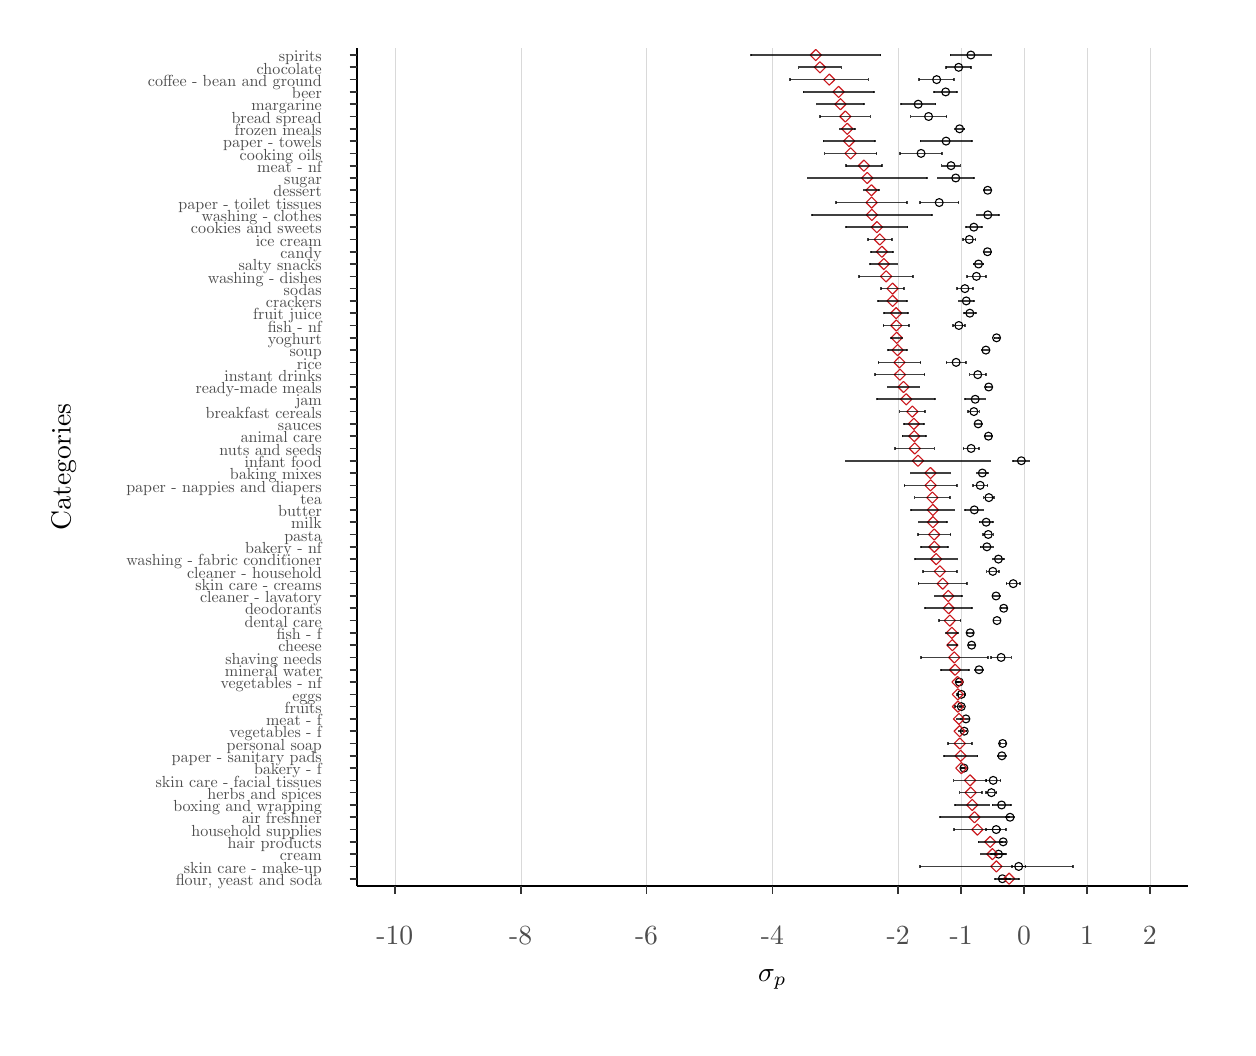
\begin{tikzpicture}[x=1pt,y=1pt]
\definecolor{fillColor}{RGB}{255,255,255}
\path[use as bounding box,fill=fillColor,fill opacity=0.00] (0,0) rectangle (433.62,361.35);
\begin{scope}
\path[clip] (  0.00,  0.00) rectangle (433.62,361.35);
\definecolor{drawColor}{RGB}{255,255,255}
\definecolor{fillColor}{RGB}{255,255,255}

\path[draw=drawColor,line width= 0.6pt,line join=round,line cap=round,fill=fillColor] (  0.00,  0.00) rectangle (433.62,361.35);
\end{scope}
\begin{scope}
\path[clip] (119.04, 51.15) rectangle (419.17,354.12);
\definecolor{drawColor}{RGB}{255,255,255}

\path[draw=drawColor,line width= 0.3pt,line join=round] (155.42, 51.15) --
	(155.42,354.12);

\path[draw=drawColor,line width= 0.3pt,line join=round] (200.89, 51.15) --
	(200.89,354.12);

\path[draw=drawColor,line width= 0.3pt,line join=round] (246.37, 51.15) --
	(246.37,354.12);

\path[draw=drawColor,line width= 0.3pt,line join=round] (291.84, 51.15) --
	(291.84,354.12);

\path[draw=drawColor,line width= 0.3pt,line join=round] (325.95, 51.15) --
	(325.95,354.12);

\path[draw=drawColor,line width= 0.3pt,line join=round] (348.68, 51.15) --
	(348.68,354.12);

\path[draw=drawColor,line width= 0.3pt,line join=round] (371.42, 51.15) --
	(371.42,354.12);

\path[draw=drawColor,line width= 0.3pt,line join=round] (394.16, 51.15) --
	(394.16,354.12);
\definecolor{drawColor}{gray}{0.85}

\path[draw=drawColor,line width= 0.1pt,line join=round] (132.68, 51.15) --
	(132.68,354.12);

\path[draw=drawColor,line width= 0.1pt,line join=round] (178.16, 51.15) --
	(178.16,354.12);

\path[draw=drawColor,line width= 0.1pt,line join=round] (223.63, 51.15) --
	(223.63,354.12);

\path[draw=drawColor,line width= 0.1pt,line join=round] (269.10, 51.15) --
	(269.10,354.12);

\path[draw=drawColor,line width= 0.1pt,line join=round] (314.58, 51.15) --
	(314.58,354.12);

\path[draw=drawColor,line width= 0.1pt,line join=round] (337.31, 51.15) --
	(337.31,354.12);

\path[draw=drawColor,line width= 0.1pt,line join=round] (360.05, 51.15) --
	(360.05,354.12);

\path[draw=drawColor,line width= 0.1pt,line join=round] (382.79, 51.15) --
	(382.79,354.12);

\path[draw=drawColor,line width= 0.1pt,line join=round] (405.52, 51.15) --
	(405.52,354.12);
\definecolor{drawColor}{RGB}{0,0,0}

\path[draw=drawColor,line width= 0.4pt,line join=round,line cap=round] (354.98, 76.03) circle (  1.43);

\path[draw=drawColor,line width= 0.4pt,line join=round,line cap=round] (347.16,213.74) circle (  1.43);

\path[draw=drawColor,line width= 0.4pt,line join=round,line cap=round] (338.31, 93.80) circle (  1.43);

\path[draw=drawColor,line width= 0.4pt,line join=round,line cap=round] (346.61,173.76) circle (  1.43);

\path[draw=drawColor,line width= 0.4pt,line join=round,line cap=round] (344.96,200.42) circle (  1.43);

\path[draw=drawColor,line width= 0.4pt,line join=round,line cap=round] (331.71,338.13) circle (  1.43);

\path[draw=drawColor,line width= 0.4pt,line join=round,line cap=round] (351.92, 80.47) circle (  1.43);

\path[draw=drawColor,line width= 0.4pt,line join=round,line cap=round] (325.54,329.25) circle (  1.43);

\path[draw=drawColor,line width= 0.4pt,line join=round,line cap=round] (341.91,222.63) circle (  1.43);

\path[draw=drawColor,line width= 0.4pt,line join=round,line cap=round] (342.06,187.09) circle (  1.43);

\path[draw=drawColor,line width= 0.4pt,line join=round,line cap=round] (346.81,280.38) circle (  1.43);

\path[draw=drawColor,line width= 0.4pt,line join=round,line cap=round] (341.10,138.22) circle (  1.43);

\path[draw=drawColor,line width= 0.4pt,line join=round,line cap=round] (336.41,347.02) circle (  1.43);

\path[draw=drawColor,line width= 0.4pt,line join=round,line cap=round] (348.75,164.88) circle (  1.43);

\path[draw=drawColor,line width= 0.4pt,line join=round,line cap=round] (349.92,155.99) circle (  1.43);

\path[draw=drawColor,line width= 0.4pt,line join=round,line cap=round] (328.46,342.57) circle (  1.43);

\path[draw=drawColor,line width= 0.4pt,line join=round,line cap=round] (341.89,289.26) circle (  1.43);

\path[draw=drawColor,line width= 0.4pt,line join=round,line cap=round] (322.82,315.92) circle (  1.43);

\path[draw=drawColor,line width= 0.4pt,line join=round,line cap=round] (339.16,262.61) circle (  1.43);

\path[draw=drawColor,line width= 0.4pt,line join=round,line cap=round] (350.81, 62.70) circle (  1.43);

\path[draw=drawColor,line width= 0.4pt,line join=round,line cap=round] (350.25,147.11) circle (  1.43);

\path[draw=drawColor,line width= 0.4pt,line join=round,line cap=round] (352.69,151.55) circle (  1.43);

\path[draw=drawColor,line width= 0.4pt,line join=round,line cap=round] (346.89,302.59) circle (  1.43);

\path[draw=drawColor,line width= 0.4pt,line join=round,line cap=round] (337.38,120.45) circle (  1.43);

\path[draw=drawColor,line width= 0.4pt,line join=round,line cap=round] (340.56,142.67) circle (  1.43);

\path[draw=drawColor,line width= 0.4pt,line join=round,line cap=round] (336.47,253.73) circle (  1.43);

\path[draw=drawColor,line width= 0.4pt,line join=round,line cap=round] (352.20, 53.82) circle (  1.43);

\path[draw=drawColor,line width= 0.4pt,line join=round,line cap=round] (336.73,324.80) circle (  1.43);

\path[draw=drawColor,line width= 0.4pt,line join=round,line cap=round] (340.45,258.17) circle (  1.43);

\path[draw=drawColor,line width= 0.4pt,line join=round,line cap=round] (337.36,116.01) circle (  1.43);

\path[draw=drawColor,line width= 0.4pt,line join=round,line cap=round] (352.49, 67.15) circle (  1.43);

\path[draw=drawColor,line width= 0.4pt,line join=round,line cap=round] (348.24, 84.92) circle (  1.43);

\path[draw=drawColor,line width= 0.4pt,line join=round,line cap=round] (349.97, 71.59) circle (  1.43);

\path[draw=drawColor,line width= 0.4pt,line join=round,line cap=round] (340.26,284.82) circle (  1.43);

\path[draw=drawColor,line width= 0.4pt,line join=round,line cap=round] (359.06,204.86) circle (  1.43);

\path[draw=drawColor,line width= 0.4pt,line join=round,line cap=round] (343.31,235.96) circle (  1.43);

\path[draw=drawColor,line width= 0.4pt,line join=round,line cap=round] (342.39,227.07) circle (  1.43);

\path[draw=drawColor,line width= 0.4pt,line join=round,line cap=round] (321.78,333.69) circle (  1.43);

\path[draw=drawColor,line width= 0.4pt,line join=round,line cap=round] (339.03,111.57) circle (  1.43);

\path[draw=drawColor,line width= 0.4pt,line join=round,line cap=round] (333.65,311.48) circle (  1.43);

\path[draw=drawColor,line width= 0.4pt,line join=round,line cap=round] (346.35,182.65) circle (  1.43);

\path[draw=drawColor,line width= 0.4pt,line join=round,line cap=round] (343.78,129.34) circle (  1.43);

\path[draw=drawColor,line width= 0.4pt,line join=round,line cap=round] (340.91,209.30) circle (  1.43);

\path[draw=drawColor,line width= 0.4pt,line join=round,line cap=round] (344.19,195.97) circle (  1.43);

\path[draw=drawColor,line width= 0.4pt,line join=round,line cap=round] (352.03, 98.24) circle (  1.43);

\path[draw=drawColor,line width= 0.4pt,line join=round,line cap=round] (329.38,298.15) circle (  1.43);

\path[draw=drawColor,line width= 0.4pt,line join=round,line cap=round] (331.86,320.36) circle (  1.43);

\path[draw=drawColor,line width= 0.4pt,line join=round,line cap=round] (347.10,178.21) circle (  1.43);

\path[draw=drawColor,line width= 0.4pt,line join=round,line cap=round] (352.31,102.69) circle (  1.43);

\path[draw=drawColor,line width= 0.4pt,line join=round,line cap=round] (347.26,231.51) circle (  1.43);

\path[draw=drawColor,line width= 0.4pt,line join=round,line cap=round] (335.49,240.40) circle (  1.43);

\path[draw=drawColor,line width= 0.4pt,line join=round,line cap=round] (343.58,275.94) circle (  1.43);

\path[draw=drawColor,line width= 0.4pt,line join=round,line cap=round] (343.46,218.19) circle (  1.43);

\path[draw=drawColor,line width= 0.4pt,line join=round,line cap=round] (351.75,133.78) circle (  1.43);

\path[draw=drawColor,line width= 0.4pt,line join=round,line cap=round] (356.12,160.44) circle (  1.43);

\path[draw=drawColor,line width= 0.4pt,line join=round,line cap=round] (348.88, 89.36) circle (  1.43);

\path[draw=drawColor,line width= 0.4pt,line join=round,line cap=round] (358.10, 58.26) circle (  1.43);

\path[draw=drawColor,line width= 0.4pt,line join=round,line cap=round] (338.67,267.05) circle (  1.43);

\path[draw=drawColor,line width= 0.4pt,line join=round,line cap=round] (346.25,244.84) circle (  1.43);

\path[draw=drawColor,line width= 0.4pt,line join=round,line cap=round] (340.82,351.46) circle (  1.43);

\path[draw=drawColor,line width= 0.4pt,line join=round,line cap=round] (335.35,307.03) circle (  1.43);

\path[draw=drawColor,line width= 0.4pt,line join=round,line cap=round] (347.33,191.53) circle (  1.43);

\path[draw=drawColor,line width= 0.4pt,line join=round,line cap=round] (338.42,107.13) circle (  1.43);

\path[draw=drawColor,line width= 0.4pt,line join=round,line cap=round] (336.64,124.90) circle (  1.43);

\path[draw=drawColor,line width= 0.4pt,line join=round,line cap=round] (346.94,293.71) circle (  1.43);

\path[draw=drawColor,line width= 0.4pt,line join=round,line cap=round] (342.83,271.49) circle (  1.43);

\path[draw=drawColor,line width= 0.4pt,line join=round,line cap=round] (350.78,169.32) circle (  1.43);

\path[draw=drawColor,line width= 0.4pt,line join=round,line cap=round] (350.10,249.28) circle (  1.43);
\definecolor{drawColor}{RGB}{0,0,0}

\path[draw=drawColor,draw opacity=0.75,line width= 0.6pt,line join=round] (356.53, 75.59) --
	(356.53, 76.48);

\path[draw=drawColor,draw opacity=0.75,line width= 0.6pt,line join=round] (356.53, 76.03) --
	(353.44, 76.03);

\path[draw=drawColor,draw opacity=0.75,line width= 0.6pt,line join=round] (353.44, 75.59) --
	(353.44, 76.48);

\path[draw=drawColor,draw opacity=0.75,line width= 0.6pt,line join=round] (348.40,213.30) --
	(348.40,214.19);

\path[draw=drawColor,draw opacity=0.75,line width= 0.6pt,line join=round] (348.40,213.74) --
	(345.92,213.74);

\path[draw=drawColor,draw opacity=0.75,line width= 0.6pt,line join=round] (345.92,213.30) --
	(345.92,214.19);

\path[draw=drawColor,draw opacity=0.75,line width= 0.6pt,line join=round] (338.64, 93.36) --
	(338.64, 94.24);

\path[draw=drawColor,draw opacity=0.75,line width= 0.6pt,line join=round] (338.64, 93.80) --
	(337.98, 93.80);

\path[draw=drawColor,draw opacity=0.75,line width= 0.6pt,line join=round] (337.98, 93.36) --
	(337.98, 94.24);

\path[draw=drawColor,draw opacity=0.75,line width= 0.6pt,line join=round] (348.96,173.32) --
	(348.96,174.21);

\path[draw=drawColor,draw opacity=0.75,line width= 0.6pt,line join=round] (348.96,173.76) --
	(344.27,173.76);

\path[draw=drawColor,draw opacity=0.75,line width= 0.6pt,line join=round] (344.27,173.32) --
	(344.27,174.21);

\path[draw=drawColor,draw opacity=0.75,line width= 0.6pt,line join=round] (347.03,199.97) --
	(347.03,200.86);

\path[draw=drawColor,draw opacity=0.75,line width= 0.6pt,line join=round] (347.03,200.42) --
	(342.88,200.42);

\path[draw=drawColor,draw opacity=0.75,line width= 0.6pt,line join=round] (342.88,199.97) --
	(342.88,200.86);

\path[draw=drawColor,draw opacity=0.75,line width= 0.6pt,line join=round] (335.81,337.69) --
	(335.81,338.57);

\path[draw=drawColor,draw opacity=0.75,line width= 0.6pt,line join=round] (335.81,338.13) --
	(327.61,338.13);

\path[draw=drawColor,draw opacity=0.75,line width= 0.6pt,line join=round] (327.61,337.69) --
	(327.61,338.57);

\path[draw=drawColor,draw opacity=0.75,line width= 0.6pt,line join=round] (355.22, 80.03) --
	(355.22, 80.92);

\path[draw=drawColor,draw opacity=0.75,line width= 0.6pt,line join=round] (355.22, 80.47) --
	(348.62, 80.47);

\path[draw=drawColor,draw opacity=0.75,line width= 0.6pt,line join=round] (348.62, 80.03) --
	(348.62, 80.92);

\path[draw=drawColor,draw opacity=0.75,line width= 0.6pt,line join=round] (332.06,328.80) --
	(332.06,329.69);

\path[draw=drawColor,draw opacity=0.75,line width= 0.6pt,line join=round] (332.06,329.25) --
	(319.03,329.25);

\path[draw=drawColor,draw opacity=0.75,line width= 0.6pt,line join=round] (319.03,328.80) --
	(319.03,329.69);

\path[draw=drawColor,draw opacity=0.75,line width= 0.6pt,line join=round] (343.93,222.18) --
	(343.93,223.07);

\path[draw=drawColor,draw opacity=0.75,line width= 0.6pt,line join=round] (343.93,222.63) --
	(339.88,222.63);

\path[draw=drawColor,draw opacity=0.75,line width= 0.6pt,line join=round] (339.88,222.18) --
	(339.88,223.07);

\path[draw=drawColor,draw opacity=0.75,line width= 0.6pt,line join=round] (345.38,186.65) --
	(345.38,187.53);

\path[draw=drawColor,draw opacity=0.75,line width= 0.6pt,line join=round] (345.38,187.09) --
	(338.73,187.09);

\path[draw=drawColor,draw opacity=0.75,line width= 0.6pt,line join=round] (338.73,186.65) --
	(338.73,187.53);

\path[draw=drawColor,draw opacity=0.75,line width= 0.6pt,line join=round] (348.24,279.94) --
	(348.24,280.82);

\path[draw=drawColor,draw opacity=0.75,line width= 0.6pt,line join=round] (348.24,280.38) --
	(345.38,280.38);

\path[draw=drawColor,draw opacity=0.75,line width= 0.6pt,line join=round] (345.38,279.94) --
	(345.38,280.82);

\path[draw=drawColor,draw opacity=0.75,line width= 0.6pt,line join=round] (342.07,137.78) --
	(342.07,138.67);

\path[draw=drawColor,draw opacity=0.75,line width= 0.6pt,line join=round] (342.07,138.22) --
	(340.14,138.22);

\path[draw=drawColor,draw opacity=0.75,line width= 0.6pt,line join=round] (340.14,137.78) --
	(340.14,138.67);

\path[draw=drawColor,draw opacity=0.75,line width= 0.6pt,line join=round] (340.97,346.57) --
	(340.97,347.46);

\path[draw=drawColor,draw opacity=0.75,line width= 0.6pt,line join=round] (340.97,347.02) --
	(331.85,347.02);

\path[draw=drawColor,draw opacity=0.75,line width= 0.6pt,line join=round] (331.85,346.57) --
	(331.85,347.46);

\path[draw=drawColor,draw opacity=0.75,line width= 0.6pt,line join=round] (351.03,164.43) --
	(351.03,165.32);

\path[draw=drawColor,draw opacity=0.75,line width= 0.6pt,line join=round] (351.03,164.88) --
	(346.48,164.88);

\path[draw=drawColor,draw opacity=0.75,line width= 0.6pt,line join=round] (346.48,164.43) --
	(346.48,165.32);

\path[draw=drawColor,draw opacity=0.75,line width= 0.6pt,line join=round] (351.23,155.55) --
	(351.23,156.44);

\path[draw=drawColor,draw opacity=0.75,line width= 0.6pt,line join=round] (351.23,155.99) --
	(348.60,155.99);

\path[draw=drawColor,draw opacity=0.75,line width= 0.6pt,line join=round] (348.60,155.55) --
	(348.60,156.44);

\path[draw=drawColor,draw opacity=0.75,line width= 0.6pt,line join=round] (334.75,342.13) --
	(334.75,343.02);

\path[draw=drawColor,draw opacity=0.75,line width= 0.6pt,line join=round] (334.75,342.57) --
	(322.17,342.57);

\path[draw=drawColor,draw opacity=0.75,line width= 0.6pt,line join=round] (322.17,342.13) --
	(322.17,343.02);

\path[draw=drawColor,draw opacity=0.75,line width= 0.6pt,line join=round] (344.73,288.82) --
	(344.73,289.71);

\path[draw=drawColor,draw opacity=0.75,line width= 0.6pt,line join=round] (344.73,289.26) --
	(339.05,289.26);

\path[draw=drawColor,draw opacity=0.75,line width= 0.6pt,line join=round] (339.05,288.82) --
	(339.05,289.71);

\path[draw=drawColor,draw opacity=0.75,line width= 0.6pt,line join=round] (330.34,315.47) --
	(330.34,316.36);

\path[draw=drawColor,draw opacity=0.75,line width= 0.6pt,line join=round] (330.34,315.92) --
	(315.30,315.92);

\path[draw=drawColor,draw opacity=0.75,line width= 0.6pt,line join=round] (315.30,315.47) --
	(315.30,316.36);

\path[draw=drawColor,draw opacity=0.75,line width= 0.6pt,line join=round] (341.94,262.17) --
	(341.94,263.05);

\path[draw=drawColor,draw opacity=0.75,line width= 0.6pt,line join=round] (341.94,262.61) --
	(336.37,262.61);

\path[draw=drawColor,draw opacity=0.75,line width= 0.6pt,line join=round] (336.37,262.17) --
	(336.37,263.05);

\path[draw=drawColor,draw opacity=0.75,line width= 0.6pt,line join=round] (353.49, 62.26) --
	(353.49, 63.15);

\path[draw=drawColor,draw opacity=0.75,line width= 0.6pt,line join=round] (353.49, 62.70) --
	(348.13, 62.70);

\path[draw=drawColor,draw opacity=0.75,line width= 0.6pt,line join=round] (348.13, 62.26) --
	(348.13, 63.15);

\path[draw=drawColor,draw opacity=0.75,line width= 0.6pt,line join=round] (351.52,146.66) --
	(351.52,147.55);

\path[draw=drawColor,draw opacity=0.75,line width= 0.6pt,line join=round] (351.52,147.11) --
	(348.99,147.11);

\path[draw=drawColor,draw opacity=0.75,line width= 0.6pt,line join=round] (348.99,146.66) --
	(348.99,147.55);

\path[draw=drawColor,draw opacity=0.75,line width= 0.6pt,line join=round] (353.71,151.11) --
	(353.71,152.00);

\path[draw=drawColor,draw opacity=0.75,line width= 0.6pt,line join=round] (353.71,151.55) --
	(351.66,151.55);

\path[draw=drawColor,draw opacity=0.75,line width= 0.6pt,line join=round] (351.66,151.11) --
	(351.66,152.00);

\path[draw=drawColor,draw opacity=0.75,line width= 0.6pt,line join=round] (348.22,302.15) --
	(348.22,303.04);

\path[draw=drawColor,draw opacity=0.75,line width= 0.6pt,line join=round] (348.22,302.59) --
	(345.55,302.59);

\path[draw=drawColor,draw opacity=0.75,line width= 0.6pt,line join=round] (345.55,302.15) --
	(345.55,303.04);

\path[draw=drawColor,draw opacity=0.75,line width= 0.6pt,line join=round] (338.62,120.01) --
	(338.62,120.90);

\path[draw=drawColor,draw opacity=0.75,line width= 0.6pt,line join=round] (338.62,120.45) --
	(336.14,120.45);

\path[draw=drawColor,draw opacity=0.75,line width= 0.6pt,line join=round] (336.14,120.01) --
	(336.14,120.90);

\path[draw=drawColor,draw opacity=0.75,line width= 0.6pt,line join=round] (341.61,142.22) --
	(341.61,143.11);

\path[draw=drawColor,draw opacity=0.75,line width= 0.6pt,line join=round] (341.61,142.67) --
	(339.51,142.67);

\path[draw=drawColor,draw opacity=0.75,line width= 0.6pt,line join=round] (339.51,142.22) --
	(339.51,143.11);

\path[draw=drawColor,draw opacity=0.75,line width= 0.6pt,line join=round] (338.58,253.28) --
	(338.58,254.17);

\path[draw=drawColor,draw opacity=0.75,line width= 0.6pt,line join=round] (338.58,253.73) --
	(334.37,253.73);

\path[draw=drawColor,draw opacity=0.75,line width= 0.6pt,line join=round] (334.37,253.28) --
	(334.37,254.17);

\path[draw=drawColor,draw opacity=0.75,line width= 0.6pt,line join=round] (354.86, 53.37) --
	(354.86, 54.26);

\path[draw=drawColor,draw opacity=0.75,line width= 0.6pt,line join=round] (354.86, 53.82) --
	(349.53, 53.82);

\path[draw=drawColor,draw opacity=0.75,line width= 0.6pt,line join=round] (349.53, 53.37) --
	(349.53, 54.26);

\path[draw=drawColor,draw opacity=0.75,line width= 0.6pt,line join=round] (338.52,324.36) --
	(338.52,325.25);

\path[draw=drawColor,draw opacity=0.75,line width= 0.6pt,line join=round] (338.52,324.80) --
	(334.94,324.80);

\path[draw=drawColor,draw opacity=0.75,line width= 0.6pt,line join=round] (334.94,324.36) --
	(334.94,325.25);

\path[draw=drawColor,draw opacity=0.75,line width= 0.6pt,line join=round] (342.67,257.72) --
	(342.67,258.61);

\path[draw=drawColor,draw opacity=0.75,line width= 0.6pt,line join=round] (342.67,258.17) --
	(338.22,258.17);

\path[draw=drawColor,draw opacity=0.75,line width= 0.6pt,line join=round] (338.22,257.72) --
	(338.22,258.61);

\path[draw=drawColor,draw opacity=0.75,line width= 0.6pt,line join=round] (337.96,115.57) --
	(337.96,116.46);

\path[draw=drawColor,draw opacity=0.75,line width= 0.6pt,line join=round] (337.96,116.01) --
	(336.77,116.01);

\path[draw=drawColor,draw opacity=0.75,line width= 0.6pt,line join=round] (336.77,115.57) --
	(336.77,116.46);

\path[draw=drawColor,draw opacity=0.75,line width= 0.6pt,line join=round] (353.34, 66.70) --
	(353.34, 67.59);

\path[draw=drawColor,draw opacity=0.75,line width= 0.6pt,line join=round] (353.34, 67.15) --
	(351.64, 67.15);

\path[draw=drawColor,draw opacity=0.75,line width= 0.6pt,line join=round] (351.64, 66.70) --
	(351.64, 67.59);

\path[draw=drawColor,draw opacity=0.75,line width= 0.6pt,line join=round] (350.12, 84.47) --
	(350.12, 85.36);

\path[draw=drawColor,draw opacity=0.75,line width= 0.6pt,line join=round] (350.12, 84.92) --
	(346.36, 84.92);

\path[draw=drawColor,draw opacity=0.75,line width= 0.6pt,line join=round] (346.36, 84.47) --
	(346.36, 85.36);

\path[draw=drawColor,draw opacity=0.75,line width= 0.6pt,line join=round] (353.56, 71.14) --
	(353.56, 72.03);

\path[draw=drawColor,draw opacity=0.75,line width= 0.6pt,line join=round] (353.56, 71.59) --
	(346.38, 71.59);

\path[draw=drawColor,draw opacity=0.75,line width= 0.6pt,line join=round] (346.38, 71.14) --
	(346.38, 72.03);

\path[draw=drawColor,draw opacity=0.75,line width= 0.6pt,line join=round] (342.52,284.38) --
	(342.52,285.27);

\path[draw=drawColor,draw opacity=0.75,line width= 0.6pt,line join=round] (342.52,284.82) --
	(337.99,284.82);

\path[draw=drawColor,draw opacity=0.75,line width= 0.6pt,line join=round] (337.99,284.38) --
	(337.99,285.27);

\path[draw=drawColor,draw opacity=0.75,line width= 0.6pt,line join=round] (361.98,204.42) --
	(361.98,205.30);

\path[draw=drawColor,draw opacity=0.75,line width= 0.6pt,line join=round] (361.98,204.86) --
	(356.15,204.86);

\path[draw=drawColor,draw opacity=0.75,line width= 0.6pt,line join=round] (356.15,204.42) --
	(356.15,205.30);

\path[draw=drawColor,draw opacity=0.75,line width= 0.6pt,line join=round] (346.26,235.51) --
	(346.26,236.40);

\path[draw=drawColor,draw opacity=0.75,line width= 0.6pt,line join=round] (346.26,235.96) --
	(340.37,235.96);

\path[draw=drawColor,draw opacity=0.75,line width= 0.6pt,line join=round] (340.37,235.51) --
	(340.37,236.40);

\path[draw=drawColor,draw opacity=0.75,line width= 0.6pt,line join=round] (346.10,226.63) --
	(346.10,227.52);

\path[draw=drawColor,draw opacity=0.75,line width= 0.6pt,line join=round] (346.10,227.07) --
	(338.67,227.07);

\path[draw=drawColor,draw opacity=0.75,line width= 0.6pt,line join=round] (338.67,226.63) --
	(338.67,227.52);

\path[draw=drawColor,draw opacity=0.75,line width= 0.6pt,line join=round] (328.08,333.24) --
	(328.08,334.13);

\path[draw=drawColor,draw opacity=0.75,line width= 0.6pt,line join=round] (328.08,333.69) --
	(315.49,333.69);

\path[draw=drawColor,draw opacity=0.75,line width= 0.6pt,line join=round] (315.49,333.24) --
	(315.49,334.13);

\path[draw=drawColor,draw opacity=0.75,line width= 0.6pt,line join=round] (339.93,111.13) --
	(339.93,112.01);

\path[draw=drawColor,draw opacity=0.75,line width= 0.6pt,line join=round] (339.93,111.57) --
	(338.14,111.57);

\path[draw=drawColor,draw opacity=0.75,line width= 0.6pt,line join=round] (338.14,111.13) --
	(338.14,112.01);

\path[draw=drawColor,draw opacity=0.75,line width= 0.6pt,line join=round] (337.06,311.03) --
	(337.06,311.92);

\path[draw=drawColor,draw opacity=0.75,line width= 0.6pt,line join=round] (337.06,311.48) --
	(330.23,311.48);

\path[draw=drawColor,draw opacity=0.75,line width= 0.6pt,line join=round] (330.23,311.03) --
	(330.23,311.92);

\path[draw=drawColor,draw opacity=0.75,line width= 0.6pt,line join=round] (348.82,182.20) --
	(348.82,183.09);

\path[draw=drawColor,draw opacity=0.75,line width= 0.6pt,line join=round] (348.82,182.65) --
	(343.88,182.65);

\path[draw=drawColor,draw opacity=0.75,line width= 0.6pt,line join=round] (343.88,182.20) --
	(343.88,183.09);

\path[draw=drawColor,draw opacity=0.75,line width= 0.6pt,line join=round] (345.31,128.90) --
	(345.31,129.78);

\path[draw=drawColor,draw opacity=0.75,line width= 0.6pt,line join=round] (345.31,129.34) --
	(342.24,129.34);

\path[draw=drawColor,draw opacity=0.75,line width= 0.6pt,line join=round] (342.24,128.90) --
	(342.24,129.78);

\path[draw=drawColor,draw opacity=0.75,line width= 0.6pt,line join=round] (343.69,208.86) --
	(343.69,209.75);

\path[draw=drawColor,draw opacity=0.75,line width= 0.6pt,line join=round] (343.69,209.30) --
	(338.14,209.30);

\path[draw=drawColor,draw opacity=0.75,line width= 0.6pt,line join=round] (338.14,208.86) --
	(338.14,209.75);

\path[draw=drawColor,draw opacity=0.75,line width= 0.6pt,line join=round] (346.84,195.53) --
	(346.84,196.42);

\path[draw=drawColor,draw opacity=0.75,line width= 0.6pt,line join=round] (346.84,195.97) --
	(341.54,195.97);

\path[draw=drawColor,draw opacity=0.75,line width= 0.6pt,line join=round] (341.54,195.53) --
	(341.54,196.42);

\path[draw=drawColor,draw opacity=0.75,line width= 0.6pt,line join=round] (353.63, 97.80) --
	(353.63, 98.69);

\path[draw=drawColor,draw opacity=0.75,line width= 0.6pt,line join=round] (353.63, 98.24) --
	(350.43, 98.24);

\path[draw=drawColor,draw opacity=0.75,line width= 0.6pt,line join=round] (350.43, 97.80) --
	(350.43, 98.69);

\path[draw=drawColor,draw opacity=0.75,line width= 0.6pt,line join=round] (336.39,297.70) --
	(336.39,298.59);

\path[draw=drawColor,draw opacity=0.75,line width= 0.6pt,line join=round] (336.39,298.15) --
	(322.38,298.15);

\path[draw=drawColor,draw opacity=0.75,line width= 0.6pt,line join=round] (322.38,297.70) --
	(322.38,298.59);

\path[draw=drawColor,draw opacity=0.75,line width= 0.6pt,line join=round] (341.13,319.92) --
	(341.13,320.81);

\path[draw=drawColor,draw opacity=0.75,line width= 0.6pt,line join=round] (341.13,320.36) --
	(322.59,320.36);

\path[draw=drawColor,draw opacity=0.75,line width= 0.6pt,line join=round] (322.59,319.92) --
	(322.59,320.81);

\path[draw=drawColor,draw opacity=0.75,line width= 0.6pt,line join=round] (348.98,177.76) --
	(348.98,178.65);

\path[draw=drawColor,draw opacity=0.75,line width= 0.6pt,line join=round] (348.98,178.21) --
	(345.21,178.21);

\path[draw=drawColor,draw opacity=0.75,line width= 0.6pt,line join=round] (345.21,177.76) --
	(345.21,178.65);

\path[draw=drawColor,draw opacity=0.75,line width= 0.6pt,line join=round] (353.29,102.24) --
	(353.29,103.13);

\path[draw=drawColor,draw opacity=0.75,line width= 0.6pt,line join=round] (353.29,102.69) --
	(351.33,102.69);

\path[draw=drawColor,draw opacity=0.75,line width= 0.6pt,line join=round] (351.33,102.24) --
	(351.33,103.13);

\path[draw=drawColor,draw opacity=0.75,line width= 0.6pt,line join=round] (348.25,231.07) --
	(348.25,231.96);

\path[draw=drawColor,draw opacity=0.75,line width= 0.6pt,line join=round] (348.25,231.51) --
	(346.27,231.51);

\path[draw=drawColor,draw opacity=0.75,line width= 0.6pt,line join=round] (346.27,231.07) --
	(346.27,231.96);

\path[draw=drawColor,draw opacity=0.75,line width= 0.6pt,line join=round] (339.01,239.95) --
	(339.01,240.84);

\path[draw=drawColor,draw opacity=0.75,line width= 0.6pt,line join=round] (339.01,240.40) --
	(331.97,240.40);

\path[draw=drawColor,draw opacity=0.75,line width= 0.6pt,line join=round] (331.97,239.95) --
	(331.97,240.84);

\path[draw=drawColor,draw opacity=0.75,line width= 0.6pt,line join=round] (345.42,275.49) --
	(345.42,276.38);

\path[draw=drawColor,draw opacity=0.75,line width= 0.6pt,line join=round] (345.42,275.94) --
	(341.73,275.94);

\path[draw=drawColor,draw opacity=0.75,line width= 0.6pt,line join=round] (341.73,275.49) --
	(341.73,276.38);

\path[draw=drawColor,draw opacity=0.75,line width= 0.6pt,line join=round] (344.76,217.74) --
	(344.76,218.63);

\path[draw=drawColor,draw opacity=0.75,line width= 0.6pt,line join=round] (344.76,218.19) --
	(342.17,218.19);

\path[draw=drawColor,draw opacity=0.75,line width= 0.6pt,line join=round] (342.17,217.74) --
	(342.17,218.63);

\path[draw=drawColor,draw opacity=0.75,line width= 0.6pt,line join=round] (355.47,133.34) --
	(355.47,134.23);

\path[draw=drawColor,draw opacity=0.75,line width= 0.6pt,line join=round] (355.47,133.78) --
	(348.03,133.78);

\path[draw=drawColor,draw opacity=0.75,line width= 0.6pt,line join=round] (348.03,133.34) --
	(348.03,134.23);

\path[draw=drawColor,draw opacity=0.75,line width= 0.6pt,line join=round] (358.58,159.99) --
	(358.58,160.88);

\path[draw=drawColor,draw opacity=0.75,line width= 0.6pt,line join=round] (358.58,160.44) --
	(353.67,160.44);

\path[draw=drawColor,draw opacity=0.75,line width= 0.6pt,line join=round] (353.67,159.99) --
	(353.67,160.88);

\path[draw=drawColor,draw opacity=0.75,line width= 0.6pt,line join=round] (351.54, 88.91) --
	(351.54, 89.80);

\path[draw=drawColor,draw opacity=0.75,line width= 0.6pt,line join=round] (351.54, 89.36) --
	(346.22, 89.36);

\path[draw=drawColor,draw opacity=0.75,line width= 0.6pt,line join=round] (346.22, 88.91) --
	(346.22, 89.80);

\path[draw=drawColor,draw opacity=0.75,line width= 0.6pt,line join=round] (360.56, 57.82) --
	(360.56, 58.71);

\path[draw=drawColor,draw opacity=0.75,line width= 0.6pt,line join=round] (360.56, 58.26) --
	(355.64, 58.26);

\path[draw=drawColor,draw opacity=0.75,line width= 0.6pt,line join=round] (355.64, 57.82) --
	(355.64, 58.71);

\path[draw=drawColor,draw opacity=0.75,line width= 0.6pt,line join=round] (341.61,266.61) --
	(341.61,267.50);

\path[draw=drawColor,draw opacity=0.75,line width= 0.6pt,line join=round] (341.61,267.05) --
	(335.74,267.05);

\path[draw=drawColor,draw opacity=0.75,line width= 0.6pt,line join=round] (335.74,266.61) --
	(335.74,267.50);

\path[draw=drawColor,draw opacity=0.75,line width= 0.6pt,line join=round] (347.58,244.40) --
	(347.58,245.29);

\path[draw=drawColor,draw opacity=0.75,line width= 0.6pt,line join=round] (347.58,244.84) --
	(344.93,244.84);

\path[draw=drawColor,draw opacity=0.75,line width= 0.6pt,line join=round] (344.93,244.40) --
	(344.93,245.29);

\path[draw=drawColor,draw opacity=0.75,line width= 0.6pt,line join=round] (348.23,351.01) --
	(348.23,351.90);

\path[draw=drawColor,draw opacity=0.75,line width= 0.6pt,line join=round] (348.23,351.46) --
	(333.41,351.46);

\path[draw=drawColor,draw opacity=0.75,line width= 0.6pt,line join=round] (333.41,351.01) --
	(333.41,351.90);

\path[draw=drawColor,draw opacity=0.75,line width= 0.6pt,line join=round] (341.93,306.59) --
	(341.93,307.48);

\path[draw=drawColor,draw opacity=0.75,line width= 0.6pt,line join=round] (341.93,307.03) --
	(328.78,307.03);

\path[draw=drawColor,draw opacity=0.75,line width= 0.6pt,line join=round] (328.78,306.59) --
	(328.78,307.48);

\path[draw=drawColor,draw opacity=0.75,line width= 0.6pt,line join=round] (349.24,191.09) --
	(349.24,191.98);

\path[draw=drawColor,draw opacity=0.75,line width= 0.6pt,line join=round] (349.24,191.53) --
	(345.41,191.53);

\path[draw=drawColor,draw opacity=0.75,line width= 0.6pt,line join=round] (345.41,191.09) --
	(345.41,191.98);

\path[draw=drawColor,draw opacity=0.75,line width= 0.6pt,line join=round] (339.27,106.68) --
	(339.27,107.57);

\path[draw=drawColor,draw opacity=0.75,line width= 0.6pt,line join=round] (339.27,107.13) --
	(337.56,107.13);

\path[draw=drawColor,draw opacity=0.75,line width= 0.6pt,line join=round] (337.56,106.68) --
	(337.56,107.57);

\path[draw=drawColor,draw opacity=0.75,line width= 0.6pt,line join=round] (337.37,124.45) --
	(337.37,125.34);

\path[draw=drawColor,draw opacity=0.75,line width= 0.6pt,line join=round] (337.37,124.90) --
	(335.91,124.90);

\path[draw=drawColor,draw opacity=0.75,line width= 0.6pt,line join=round] (335.91,124.45) --
	(335.91,125.34);

\path[draw=drawColor,draw opacity=0.75,line width= 0.6pt,line join=round] (350.96,293.26) --
	(350.96,294.15);

\path[draw=drawColor,draw opacity=0.75,line width= 0.6pt,line join=round] (350.96,293.71) --
	(342.91,293.71);

\path[draw=drawColor,draw opacity=0.75,line width= 0.6pt,line join=round] (342.91,293.26) --
	(342.91,294.15);

\path[draw=drawColor,draw opacity=0.75,line width= 0.6pt,line join=round] (346.23,271.05) --
	(346.23,271.94);

\path[draw=drawColor,draw opacity=0.75,line width= 0.6pt,line join=round] (346.23,271.49) --
	(339.42,271.49);

\path[draw=drawColor,draw opacity=0.75,line width= 0.6pt,line join=round] (339.42,271.05) --
	(339.42,271.94);

\path[draw=drawColor,draw opacity=0.75,line width= 0.6pt,line join=round] (352.90,168.88) --
	(352.90,169.76);

\path[draw=drawColor,draw opacity=0.75,line width= 0.6pt,line join=round] (352.90,169.32) --
	(348.66,169.32);

\path[draw=drawColor,draw opacity=0.75,line width= 0.6pt,line join=round] (348.66,168.88) --
	(348.66,169.76);

\path[draw=drawColor,draw opacity=0.75,line width= 0.6pt,line join=round] (350.87,248.84) --
	(350.87,249.73);

\path[draw=drawColor,draw opacity=0.75,line width= 0.6pt,line join=round] (350.87,249.28) --
	(349.33,249.28);

\path[draw=drawColor,draw opacity=0.75,line width= 0.6pt,line join=round] (349.33,248.84) --
	(349.33,249.73);
\definecolor{drawColor}{RGB}{203,24,29}

\path[draw=drawColor,line width= 0.4pt,line join=round,line cap=round] (340.10, 76.03) --
	(342.12, 78.05) --
	(344.13, 76.03) --
	(342.12, 74.01) --
	cycle;

\path[draw=drawColor,line width= 0.4pt,line join=round,line cap=round] (318.35,213.74) --
	(320.37,215.76) --
	(322.38,213.74) --
	(320.37,211.73) --
	cycle;

\path[draw=drawColor,line width= 0.4pt,line join=round,line cap=round] (335.36, 93.80) --
	(337.37, 95.82) --
	(339.39, 93.80) --
	(337.37, 91.78) --
	cycle;

\path[draw=drawColor,line width= 0.4pt,line join=round,line cap=round] (325.62,173.76) --
	(327.64,175.78) --
	(329.66,173.76) --
	(327.64,171.75) --
	cycle;

\path[draw=drawColor,line width= 0.4pt,line join=round,line cap=round] (324.21,200.42) --
	(326.22,202.43) --
	(328.24,200.42) --
	(326.22,198.40) --
	cycle;

\path[draw=drawColor,line width= 0.4pt,line join=round,line cap=round] (290.99,338.13) --
	(293.01,340.15) --
	(295.03,338.13) --
	(293.01,336.11) --
	cycle;

\path[draw=drawColor,line width= 0.4pt,line join=round,line cap=round] (339.30, 80.47) --
	(341.31, 82.49) --
	(343.33, 80.47) --
	(341.31, 78.46) --
	cycle;

\path[draw=drawColor,line width= 0.4pt,line join=round,line cap=round] (293.43,329.25) --
	(295.45,331.26) --
	(297.46,329.25) --
	(295.45,327.23) --
	cycle;

\path[draw=drawColor,line width= 0.4pt,line join=round,line cap=round] (317.66,222.63) --
	(319.67,224.65) --
	(321.69,222.63) --
	(319.67,220.61) --
	cycle;

\path[draw=drawColor,line width= 0.4pt,line join=round,line cap=round] (325.05,187.09) --
	(327.07,189.11) --
	(329.09,187.09) --
	(327.07,185.07) --
	cycle;

\path[draw=drawColor,line width= 0.4pt,line join=round,line cap=round] (306.65,280.38) --
	(308.67,282.40) --
	(310.68,280.38) --
	(308.67,278.36) --
	cycle;

\path[draw=drawColor,line width= 0.4pt,line join=round,line cap=round] (332.11,138.22) --
	(334.12,140.24) --
	(336.14,138.22) --
	(334.12,136.21) --
	cycle;

\path[draw=drawColor,line width= 0.4pt,line join=round,line cap=round] (284.27,347.02) --
	(286.29,349.03) --
	(288.31,347.02) --
	(286.29,345.00) --
	cycle;

\path[draw=drawColor,line width= 0.4pt,line join=round,line cap=round] (327.61,164.88) --
	(329.63,166.90) --
	(331.64,164.88) --
	(329.63,162.86) --
	cycle;

\path[draw=drawColor,line width= 0.4pt,line join=round,line cap=round] (330.63,155.99) --
	(332.65,158.01) --
	(334.67,155.99) --
	(332.65,153.98) --
	cycle;

\path[draw=drawColor,line width= 0.4pt,line join=round,line cap=round] (287.63,342.57) --
	(289.65,344.59) --
	(291.67,342.57) --
	(289.65,340.56) --
	cycle;

\path[draw=drawColor,line width= 0.4pt,line join=round,line cap=round] (304.86,289.26) --
	(306.88,291.28) --
	(308.90,289.26) --
	(306.88,287.25) --
	cycle;

\path[draw=drawColor,line width= 0.4pt,line join=round,line cap=round] (295.35,315.92) --
	(297.36,317.94) --
	(299.38,315.92) --
	(297.36,313.90) --
	cycle;

\path[draw=drawColor,line width= 0.4pt,line join=round,line cap=round] (310.50,262.61) --
	(312.52,264.63) --
	(314.54,262.61) --
	(312.52,260.59) --
	cycle;

\path[draw=drawColor,line width= 0.4pt,line join=round,line cap=round] (346.60, 62.70) --
	(348.62, 64.72) --
	(350.64, 62.70) --
	(348.62, 60.69) --
	cycle;

\path[draw=drawColor,line width= 0.4pt,line join=round,line cap=round] (331.20,147.11) --
	(333.22,149.13) --
	(335.23,147.11) --
	(333.22,145.09) --
	cycle;

\path[draw=drawColor,line width= 0.4pt,line join=round,line cap=round] (330.77,151.55) --
	(332.79,153.57) --
	(334.81,151.55) --
	(332.79,149.53) --
	cycle;

\path[draw=drawColor,line width= 0.4pt,line join=round,line cap=round] (302.86,302.59) --
	(304.88,304.61) --
	(306.90,302.59) --
	(304.88,300.57) --
	cycle;

\path[draw=drawColor,line width= 0.4pt,line join=round,line cap=round] (334.10,120.45) --
	(336.11,122.47) --
	(338.13,120.45) --
	(336.11,118.44) --
	cycle;

\path[draw=drawColor,line width= 0.4pt,line join=round,line cap=round] (331.92,142.67) --
	(333.94,144.68) --
	(335.96,142.67) --
	(333.94,140.65) --
	cycle;

\path[draw=drawColor,line width= 0.4pt,line join=round,line cap=round] (311.87,253.73) --
	(313.89,255.74) --
	(315.91,253.73) --
	(313.89,251.71) --
	cycle;

\path[draw=drawColor,line width= 0.4pt,line join=round,line cap=round] (352.62, 53.82) --
	(354.64, 55.84) --
	(356.66, 53.82) --
	(354.64, 51.80) --
	cycle;

\path[draw=drawColor,line width= 0.4pt,line join=round,line cap=round] (294.12,324.80) --
	(296.14,326.82) --
	(298.16,324.80) --
	(296.14,322.79) --
	cycle;

\path[draw=drawColor,line width= 0.4pt,line join=round,line cap=round] (311.80,258.17) --
	(313.81,260.19) --
	(315.83,258.17) --
	(313.81,256.15) --
	cycle;

\path[draw=drawColor,line width= 0.4pt,line join=round,line cap=round] (334.14,116.01) --
	(336.16,118.03) --
	(338.18,116.01) --
	(336.16,113.99) --
	cycle;

\path[draw=drawColor,line width= 0.4pt,line join=round,line cap=round] (345.79, 67.15) --
	(347.81, 69.16) --
	(349.82, 67.15) --
	(347.81, 65.13) --
	cycle;

\path[draw=drawColor,line width= 0.4pt,line join=round,line cap=round] (338.73, 84.92) --
	(340.75, 86.93) --
	(342.77, 84.92) --
	(340.75, 82.90) --
	cycle;

\path[draw=drawColor,line width= 0.4pt,line join=round,line cap=round] (341.16, 71.59) --
	(343.18, 73.61) --
	(345.19, 71.59) --
	(343.18, 69.57) --
	cycle;

\path[draw=drawColor,line width= 0.4pt,line join=round,line cap=round] (305.89,284.82) --
	(307.91,286.84) --
	(309.92,284.82) --
	(307.91,282.80) --
	cycle;

\path[draw=drawColor,line width= 0.4pt,line join=round,line cap=round] (319.71,204.86) --
	(321.73,206.88) --
	(323.75,204.86) --
	(321.73,202.84) --
	cycle;

\path[draw=drawColor,line width= 0.4pt,line join=round,line cap=round] (313.17,235.96) --
	(315.19,237.97) --
	(317.21,235.96) --
	(315.19,233.94) --
	cycle;

\path[draw=drawColor,line width= 0.4pt,line join=round,line cap=round] (315.43,227.07) --
	(317.45,229.09) --
	(319.47,227.07) --
	(317.45,225.05) --
	cycle;

\path[draw=drawColor,line width= 0.4pt,line join=round,line cap=round] (291.67,333.69) --
	(293.69,335.71) --
	(295.71,333.69) --
	(293.69,331.67) --
	cycle;

\path[draw=drawColor,line width= 0.4pt,line join=round,line cap=round] (334.50,111.57) --
	(336.52,113.59) --
	(338.53,111.57) --
	(336.52,109.55) --
	cycle;

\path[draw=drawColor,line width= 0.4pt,line join=round,line cap=round] (300.15,311.48) --
	(302.17,313.49) --
	(304.19,311.48) --
	(302.17,309.46) --
	cycle;

\path[draw=drawColor,line width= 0.4pt,line join=round,line cap=round] (325.09,182.65) --
	(327.10,184.67) --
	(329.12,182.65) --
	(327.10,180.63) --
	cycle;

\path[draw=drawColor,line width= 0.4pt,line join=round,line cap=round] (333.10,129.34) --
	(335.12,131.36) --
	(337.14,129.34) --
	(335.12,127.32) --
	cycle;

\path[draw=drawColor,line width= 0.4pt,line join=round,line cap=round] (318.53,209.30) --
	(320.55,211.32) --
	(322.57,209.30) --
	(320.55,207.28) --
	cycle;

\path[draw=drawColor,line width= 0.4pt,line join=round,line cap=round] (324.23,195.97) --
	(326.25,197.99) --
	(328.27,195.97) --
	(326.25,193.96) --
	cycle;

\path[draw=drawColor,line width= 0.4pt,line join=round,line cap=round] (335.11, 98.24) --
	(337.13,100.26) --
	(339.15, 98.24) --
	(337.13, 96.23) --
	cycle;

\path[draw=drawColor,line width= 0.4pt,line join=round,line cap=round] (302.94,298.15) --
	(304.96,300.17) --
	(306.97,298.15) --
	(304.96,296.13) --
	cycle;

\path[draw=drawColor,line width= 0.4pt,line join=round,line cap=round] (294.79,320.36) --
	(296.81,322.38) --
	(298.82,320.36) --
	(296.81,318.34) --
	cycle;

\path[draw=drawColor,line width= 0.4pt,line join=round,line cap=round] (325.54,178.21) --
	(327.56,180.22) --
	(329.58,178.21) --
	(327.56,176.19) --
	cycle;

\path[draw=drawColor,line width= 0.4pt,line join=round,line cap=round] (334.80,102.69) --
	(336.82,104.70) --
	(338.83,102.69) --
	(336.82,100.67) --
	cycle;

\path[draw=drawColor,line width= 0.4pt,line join=round,line cap=round] (314.47,231.51) --
	(316.49,233.53) --
	(318.50,231.51) --
	(316.49,229.50) --
	cycle;

\path[draw=drawColor,line width= 0.4pt,line join=round,line cap=round] (313.01,240.40) --
	(315.02,242.42) --
	(317.04,240.40) --
	(315.02,238.38) --
	cycle;

\path[draw=drawColor,line width= 0.4pt,line join=round,line cap=round] (307.35,275.94) --
	(309.37,277.95) --
	(311.39,275.94) --
	(309.37,273.92) --
	cycle;

\path[draw=drawColor,line width= 0.4pt,line join=round,line cap=round] (318.20,218.19) --
	(320.21,220.20) --
	(322.23,218.19) --
	(320.21,216.17) --
	cycle;

\path[draw=drawColor,line width= 0.4pt,line join=round,line cap=round] (332.81,133.78) --
	(334.83,135.80) --
	(336.85,133.78) --
	(334.83,131.76) --
	cycle;

\path[draw=drawColor,line width= 0.4pt,line join=round,line cap=round] (328.63,160.44) --
	(330.65,162.45) --
	(332.66,160.44) --
	(330.65,158.42) --
	cycle;

\path[draw=drawColor,line width= 0.4pt,line join=round,line cap=round] (338.51, 89.36) --
	(340.52, 91.38) --
	(342.54, 89.36) --
	(340.52, 87.34) --
	cycle;

\path[draw=drawColor,line width= 0.4pt,line join=round,line cap=round] (348.02, 58.26) --
	(350.04, 60.28) --
	(352.05, 58.26) --
	(350.04, 56.24) --
	cycle;

\path[draw=drawColor,line width= 0.4pt,line join=round,line cap=round] (310.49,267.05) --
	(312.51,269.07) --
	(314.53,267.05) --
	(312.51,265.04) --
	cycle;

\path[draw=drawColor,line width= 0.4pt,line join=round,line cap=round] (312.32,244.84) --
	(314.33,246.86) --
	(316.35,244.84) --
	(314.33,242.82) --
	cycle;

\path[draw=drawColor,line width= 0.4pt,line join=round,line cap=round] (282.77,351.46) --
	(284.79,353.48) --
	(286.80,351.46) --
	(284.79,349.44) --
	cycle;

\path[draw=drawColor,line width= 0.4pt,line join=round,line cap=round] (301.35,307.03) --
	(303.36,309.05) --
	(305.38,307.03) --
	(303.36,305.02) --
	cycle;

\path[draw=drawColor,line width= 0.4pt,line join=round,line cap=round] (324.90,191.53) --
	(326.92,193.55) --
	(328.93,191.53) --
	(326.92,189.51) --
	cycle;

\path[draw=drawColor,line width= 0.4pt,line join=round,line cap=round] (334.74,107.13) --
	(336.76,109.14) --
	(338.77,107.13) --
	(336.76,105.11) --
	cycle;

\path[draw=drawColor,line width= 0.4pt,line join=round,line cap=round] (333.98,124.90) --
	(336.00,126.91) --
	(338.02,124.90) --
	(336.00,122.88) --
	cycle;

\path[draw=drawColor,line width= 0.4pt,line join=round,line cap=round] (303.04,293.71) --
	(305.05,295.72) --
	(307.07,293.71) --
	(305.05,291.69) --
	cycle;

\path[draw=drawColor,line width= 0.4pt,line join=round,line cap=round] (308.17,271.49) --
	(310.19,273.51) --
	(312.21,271.49) --
	(310.19,269.48) --
	cycle;

\path[draw=drawColor,line width= 0.4pt,line join=round,line cap=round] (326.27,169.32) --
	(328.29,171.34) --
	(330.31,169.32) --
	(328.29,167.30) --
	cycle;

\path[draw=drawColor,line width= 0.4pt,line join=round,line cap=round] (312.01,249.28) --
	(314.03,251.30) --
	(316.05,249.28) --
	(314.03,247.27) --
	cycle;
\definecolor{drawColor}{RGB}{0,0,0}

\path[draw=drawColor,draw opacity=0.75,line width= 0.6pt,line join=round] (354.66, 75.59) --
	(354.66, 76.48);

\path[draw=drawColor,draw opacity=0.75,line width= 0.6pt,line join=round] (354.66, 76.03) --
	(329.57, 76.03);

\path[draw=drawColor,draw opacity=0.75,line width= 0.6pt,line join=round] (329.57, 75.59) --
	(329.57, 76.48);

\path[draw=drawColor,draw opacity=0.75,line width= 0.6pt,line join=round] (324.66,213.30) --
	(324.66,214.19);

\path[draw=drawColor,draw opacity=0.75,line width= 0.6pt,line join=round] (324.66,213.74) --
	(316.07,213.74);

\path[draw=drawColor,draw opacity=0.75,line width= 0.6pt,line join=round] (316.07,213.30) --
	(316.07,214.19);

\path[draw=drawColor,draw opacity=0.75,line width= 0.6pt,line join=round] (337.50, 93.36) --
	(337.50, 94.24);

\path[draw=drawColor,draw opacity=0.75,line width= 0.6pt,line join=round] (337.50, 93.80) --
	(337.24, 93.80);

\path[draw=drawColor,draw opacity=0.75,line width= 0.6pt,line join=round] (337.24, 93.36) --
	(337.24, 94.24);

\path[draw=drawColor,draw opacity=0.75,line width= 0.6pt,line join=round] (332.52,173.32) --
	(332.52,174.21);

\path[draw=drawColor,draw opacity=0.75,line width= 0.6pt,line join=round] (332.52,173.76) --
	(322.76,173.76);

\path[draw=drawColor,draw opacity=0.75,line width= 0.6pt,line join=round] (322.76,173.32) --
	(322.76,174.21);

\path[draw=drawColor,draw opacity=0.75,line width= 0.6pt,line join=round] (333.42,199.97) --
	(333.42,200.86);

\path[draw=drawColor,draw opacity=0.75,line width= 0.6pt,line join=round] (333.42,200.42) --
	(319.02,200.42);

\path[draw=drawColor,draw opacity=0.75,line width= 0.6pt,line join=round] (319.02,199.97) --
	(319.02,200.86);

\path[draw=drawColor,draw opacity=0.75,line width= 0.6pt,line join=round] (305.74,337.69) --
	(305.74,338.57);

\path[draw=drawColor,draw opacity=0.75,line width= 0.6pt,line join=round] (305.74,338.13) --
	(280.28,338.13);

\path[draw=drawColor,draw opacity=0.75,line width= 0.6pt,line join=round] (280.28,337.69) --
	(280.28,338.57);

\path[draw=drawColor,draw opacity=0.75,line width= 0.6pt,line join=round] (347.53, 80.03) --
	(347.53, 80.92);

\path[draw=drawColor,draw opacity=0.75,line width= 0.6pt,line join=round] (347.53, 80.47) --
	(335.09, 80.47);

\path[draw=drawColor,draw opacity=0.75,line width= 0.6pt,line join=round] (335.09, 80.03) --
	(335.09, 80.92);

\path[draw=drawColor,draw opacity=0.75,line width= 0.6pt,line join=round] (304.54,328.80) --
	(304.54,329.69);

\path[draw=drawColor,draw opacity=0.75,line width= 0.6pt,line join=round] (304.54,329.25) --
	(286.36,329.25);

\path[draw=drawColor,draw opacity=0.75,line width= 0.6pt,line join=round] (286.36,328.80) --
	(286.36,329.69);

\path[draw=drawColor,draw opacity=0.75,line width= 0.6pt,line join=round] (324.26,222.18) --
	(324.26,223.07);

\path[draw=drawColor,draw opacity=0.75,line width= 0.6pt,line join=round] (324.26,222.63) --
	(315.08,222.63);

\path[draw=drawColor,draw opacity=0.75,line width= 0.6pt,line join=round] (315.08,222.18) --
	(315.08,223.07);

\path[draw=drawColor,draw opacity=0.75,line width= 0.6pt,line join=round] (334.85,186.65) --
	(334.85,187.53);

\path[draw=drawColor,draw opacity=0.75,line width= 0.6pt,line join=round] (334.85,187.09) --
	(319.29,187.09);

\path[draw=drawColor,draw opacity=0.75,line width= 0.6pt,line join=round] (319.29,186.65) --
	(319.29,187.53);

\path[draw=drawColor,draw opacity=0.75,line width= 0.6pt,line join=round] (312.64,279.94) --
	(312.64,280.82);

\path[draw=drawColor,draw opacity=0.75,line width= 0.6pt,line join=round] (312.64,280.38) --
	(304.70,280.38);

\path[draw=drawColor,draw opacity=0.75,line width= 0.6pt,line join=round] (304.70,279.94) --
	(304.70,280.82);

\path[draw=drawColor,draw opacity=0.75,line width= 0.6pt,line join=round] (335.85,137.78) --
	(335.85,138.67);

\path[draw=drawColor,draw opacity=0.75,line width= 0.6pt,line join=round] (335.85,138.22) --
	(332.40,138.22);

\path[draw=drawColor,draw opacity=0.75,line width= 0.6pt,line join=round] (332.40,137.78) --
	(332.40,138.67);

\path[draw=drawColor,draw opacity=0.75,line width= 0.6pt,line join=round] (294.02,346.57) --
	(294.02,347.46);

\path[draw=drawColor,draw opacity=0.75,line width= 0.6pt,line join=round] (294.02,347.02) --
	(278.56,347.02);

\path[draw=drawColor,draw opacity=0.75,line width= 0.6pt,line join=round] (278.56,346.57) --
	(278.56,347.46);

\path[draw=drawColor,draw opacity=0.75,line width= 0.6pt,line join=round] (335.79,164.43) --
	(335.79,165.32);

\path[draw=drawColor,draw opacity=0.75,line width= 0.6pt,line join=round] (335.79,164.88) --
	(323.46,164.88);

\path[draw=drawColor,draw opacity=0.75,line width= 0.6pt,line join=round] (323.46,164.43) --
	(323.46,165.32);

\path[draw=drawColor,draw opacity=0.75,line width= 0.6pt,line join=round] (337.61,155.55) --
	(337.61,156.44);

\path[draw=drawColor,draw opacity=0.75,line width= 0.6pt,line join=round] (337.61,155.99) --
	(327.69,155.99);

\path[draw=drawColor,draw opacity=0.75,line width= 0.6pt,line join=round] (327.69,155.55) --
	(327.69,156.44);

\path[draw=drawColor,draw opacity=0.75,line width= 0.6pt,line join=round] (303.78,342.13) --
	(303.78,343.02);

\path[draw=drawColor,draw opacity=0.75,line width= 0.6pt,line join=round] (303.78,342.57) --
	(275.51,342.57);

\path[draw=drawColor,draw opacity=0.75,line width= 0.6pt,line join=round] (275.51,342.13) --
	(275.51,343.02);

\path[draw=drawColor,draw opacity=0.75,line width= 0.6pt,line join=round] (317.97,288.82) --
	(317.97,289.71);

\path[draw=drawColor,draw opacity=0.75,line width= 0.6pt,line join=round] (317.97,289.26) --
	(295.79,289.26);

\path[draw=drawColor,draw opacity=0.75,line width= 0.6pt,line join=round] (295.79,288.82) --
	(295.79,289.71);

\path[draw=drawColor,draw opacity=0.75,line width= 0.6pt,line join=round] (306.75,315.47) --
	(306.75,316.36);

\path[draw=drawColor,draw opacity=0.75,line width= 0.6pt,line join=round] (306.75,315.92) --
	(287.98,315.92);

\path[draw=drawColor,draw opacity=0.75,line width= 0.6pt,line join=round] (287.98,315.47) --
	(287.98,316.36);

\path[draw=drawColor,draw opacity=0.75,line width= 0.6pt,line join=round] (317.85,262.17) --
	(317.85,263.05);

\path[draw=drawColor,draw opacity=0.75,line width= 0.6pt,line join=round] (317.85,262.61) --
	(307.19,262.61);

\path[draw=drawColor,draw opacity=0.75,line width= 0.6pt,line join=round] (307.19,262.17) --
	(307.19,263.05);

\path[draw=drawColor,draw opacity=0.75,line width= 0.6pt,line join=round] (352.90, 62.26) --
	(352.90, 63.15);

\path[draw=drawColor,draw opacity=0.75,line width= 0.6pt,line join=round] (352.90, 62.70) --
	(344.33, 62.70);

\path[draw=drawColor,draw opacity=0.75,line width= 0.6pt,line join=round] (344.33, 62.26) --
	(344.33, 63.15);

\path[draw=drawColor,draw opacity=0.75,line width= 0.6pt,line join=round] (337.10,146.66) --
	(337.10,147.55);

\path[draw=drawColor,draw opacity=0.75,line width= 0.6pt,line join=round] (337.10,147.11) --
	(329.34,147.11);

\path[draw=drawColor,draw opacity=0.75,line width= 0.6pt,line join=round] (329.34,146.66) --
	(329.34,147.55);

\path[draw=drawColor,draw opacity=0.75,line width= 0.6pt,line join=round] (341.21,151.11) --
	(341.21,152.00);

\path[draw=drawColor,draw opacity=0.75,line width= 0.6pt,line join=round] (341.21,151.55) --
	(324.36,151.55);

\path[draw=drawColor,draw opacity=0.75,line width= 0.6pt,line join=round] (324.36,151.11) --
	(324.36,152.00);

\path[draw=drawColor,draw opacity=0.75,line width= 0.6pt,line join=round] (307.69,302.15) --
	(307.69,303.04);

\path[draw=drawColor,draw opacity=0.75,line width= 0.6pt,line join=round] (307.69,302.59) --
	(302.07,302.59);

\path[draw=drawColor,draw opacity=0.75,line width= 0.6pt,line join=round] (302.07,302.15) --
	(302.07,303.04);

\path[draw=drawColor,draw opacity=0.75,line width= 0.6pt,line join=round] (336.39,120.01) --
	(336.39,120.90);

\path[draw=drawColor,draw opacity=0.75,line width= 0.6pt,line join=round] (336.39,120.45) --
	(335.84,120.45);

\path[draw=drawColor,draw opacity=0.75,line width= 0.6pt,line join=round] (335.84,120.01) --
	(335.84,120.90);

\path[draw=drawColor,draw opacity=0.75,line width= 0.6pt,line join=round] (336.17,142.22) --
	(336.17,143.11);

\path[draw=drawColor,draw opacity=0.75,line width= 0.6pt,line join=round] (336.17,142.67) --
	(331.71,142.67);

\path[draw=drawColor,draw opacity=0.75,line width= 0.6pt,line join=round] (331.71,142.22) --
	(331.71,143.11);

\path[draw=drawColor,draw opacity=0.75,line width= 0.6pt,line join=round] (318.57,253.28) --
	(318.57,254.17);

\path[draw=drawColor,draw opacity=0.75,line width= 0.6pt,line join=round] (318.57,253.73) --
	(309.21,253.73);

\path[draw=drawColor,draw opacity=0.75,line width= 0.6pt,line join=round] (309.21,253.28) --
	(309.21,254.17);

\path[draw=drawColor,draw opacity=0.75,line width= 0.6pt,line join=round] (358.33, 53.37) --
	(358.33, 54.26);

\path[draw=drawColor,draw opacity=0.75,line width= 0.6pt,line join=round] (358.33, 53.82) --
	(350.94, 53.82);

\path[draw=drawColor,draw opacity=0.75,line width= 0.6pt,line join=round] (350.94, 53.37) --
	(350.94, 54.26);

\path[draw=drawColor,draw opacity=0.75,line width= 0.6pt,line join=round] (298.88,324.36) --
	(298.88,325.25);

\path[draw=drawColor,draw opacity=0.75,line width= 0.6pt,line join=round] (298.88,324.80) --
	(293.40,324.80);

\path[draw=drawColor,draw opacity=0.75,line width= 0.6pt,line join=round] (293.40,324.36) --
	(293.40,325.25);

\path[draw=drawColor,draw opacity=0.75,line width= 0.6pt,line join=round] (318.11,257.72) --
	(318.11,258.61);

\path[draw=drawColor,draw opacity=0.75,line width= 0.6pt,line join=round] (318.11,258.17) --
	(309.52,258.17);

\path[draw=drawColor,draw opacity=0.75,line width= 0.6pt,line join=round] (309.52,257.72) --
	(309.52,258.61);

\path[draw=drawColor,draw opacity=0.75,line width= 0.6pt,line join=round] (337.26,115.57) --
	(337.26,116.46);

\path[draw=drawColor,draw opacity=0.75,line width= 0.6pt,line join=round] (337.26,116.01) --
	(335.06,116.01);

\path[draw=drawColor,draw opacity=0.75,line width= 0.6pt,line join=round] (335.06,115.57) --
	(335.06,116.46);

\path[draw=drawColor,draw opacity=0.75,line width= 0.6pt,line join=round] (352.06, 66.70) --
	(352.06, 67.59);

\path[draw=drawColor,draw opacity=0.75,line width= 0.6pt,line join=round] (352.06, 67.15) --
	(343.55, 67.15);

\path[draw=drawColor,draw opacity=0.75,line width= 0.6pt,line join=round] (343.55, 66.70) --
	(343.55, 67.59);

\path[draw=drawColor,draw opacity=0.75,line width= 0.6pt,line join=round] (344.77, 84.47) --
	(344.77, 85.36);

\path[draw=drawColor,draw opacity=0.75,line width= 0.6pt,line join=round] (344.77, 84.92) --
	(336.73, 84.92);

\path[draw=drawColor,draw opacity=0.75,line width= 0.6pt,line join=round] (336.73, 84.47) --
	(336.73, 85.36);

\path[draw=drawColor,draw opacity=0.75,line width= 0.6pt,line join=round] (351.54, 71.14) --
	(351.54, 72.03);

\path[draw=drawColor,draw opacity=0.75,line width= 0.6pt,line join=round] (351.54, 71.59) --
	(334.81, 71.59);

\path[draw=drawColor,draw opacity=0.75,line width= 0.6pt,line join=round] (334.81, 71.14) --
	(334.81, 72.03);

\path[draw=drawColor,draw opacity=0.75,line width= 0.6pt,line join=round] (312.25,284.38) --
	(312.25,285.27);

\path[draw=drawColor,draw opacity=0.75,line width= 0.6pt,line join=round] (312.25,284.82) --
	(303.56,284.82);

\path[draw=drawColor,draw opacity=0.75,line width= 0.6pt,line join=round] (303.56,284.38) --
	(303.56,285.27);

\path[draw=drawColor,draw opacity=0.75,line width= 0.6pt,line join=round] (347.90,204.42) --
	(347.90,205.30);

\path[draw=drawColor,draw opacity=0.75,line width= 0.6pt,line join=round] (347.90,204.86) --
	(295.56,204.86);

\path[draw=drawColor,draw opacity=0.75,line width= 0.6pt,line join=round] (295.56,204.42) --
	(295.56,205.30);

\path[draw=drawColor,draw opacity=0.75,line width= 0.6pt,line join=round] (324.08,235.51) --
	(324.08,236.40);

\path[draw=drawColor,draw opacity=0.75,line width= 0.6pt,line join=round] (324.08,235.96) --
	(306.29,235.96);

\path[draw=drawColor,draw opacity=0.75,line width= 0.6pt,line join=round] (306.29,235.51) --
	(306.29,236.40);

\path[draw=drawColor,draw opacity=0.75,line width= 0.6pt,line join=round] (327.90,226.63) --
	(327.90,227.52);

\path[draw=drawColor,draw opacity=0.75,line width= 0.6pt,line join=round] (327.90,227.07) --
	(307.00,227.07);

\path[draw=drawColor,draw opacity=0.75,line width= 0.6pt,line join=round] (307.00,226.63) --
	(307.00,227.52);

\path[draw=drawColor,draw opacity=0.75,line width= 0.6pt,line join=round] (302.30,333.24) --
	(302.30,334.13);

\path[draw=drawColor,draw opacity=0.75,line width= 0.6pt,line join=round] (302.30,333.69) --
	(285.08,333.69);

\path[draw=drawColor,draw opacity=0.75,line width= 0.6pt,line join=round] (285.08,333.24) --
	(285.08,334.13);

\path[draw=drawColor,draw opacity=0.75,line width= 0.6pt,line join=round] (337.36,111.13) --
	(337.36,112.01);

\path[draw=drawColor,draw opacity=0.75,line width= 0.6pt,line join=round] (337.36,111.57) --
	(335.67,111.57);

\path[draw=drawColor,draw opacity=0.75,line width= 0.6pt,line join=round] (335.67,111.13) --
	(335.67,112.01);

\path[draw=drawColor,draw opacity=0.75,line width= 0.6pt,line join=round] (308.59,311.03) --
	(308.59,311.92);

\path[draw=drawColor,draw opacity=0.75,line width= 0.6pt,line join=round] (308.59,311.48) --
	(295.75,311.48);

\path[draw=drawColor,draw opacity=0.75,line width= 0.6pt,line join=round] (295.75,311.03) --
	(295.75,311.92);

\path[draw=drawColor,draw opacity=0.75,line width= 0.6pt,line join=round] (332.30,182.20) --
	(332.30,183.09);

\path[draw=drawColor,draw opacity=0.75,line width= 0.6pt,line join=round] (332.30,182.65) --
	(321.91,182.65);

\path[draw=drawColor,draw opacity=0.75,line width= 0.6pt,line join=round] (321.91,182.20) --
	(321.91,183.09);

\path[draw=drawColor,draw opacity=0.75,line width= 0.6pt,line join=round] (340.23,128.90) --
	(340.23,129.78);

\path[draw=drawColor,draw opacity=0.75,line width= 0.6pt,line join=round] (340.23,129.34) --
	(330.01,129.34);

\path[draw=drawColor,draw opacity=0.75,line width= 0.6pt,line join=round] (330.01,128.90) --
	(330.01,129.78);

\path[draw=drawColor,draw opacity=0.75,line width= 0.6pt,line join=round] (327.66,208.86) --
	(327.66,209.75);

\path[draw=drawColor,draw opacity=0.75,line width= 0.6pt,line join=round] (327.66,209.30) --
	(313.44,209.30);

\path[draw=drawColor,draw opacity=0.75,line width= 0.6pt,line join=round] (313.44,208.86) --
	(313.44,209.75);

\path[draw=drawColor,draw opacity=0.75,line width= 0.6pt,line join=round] (335.72,195.53) --
	(335.72,196.42);

\path[draw=drawColor,draw opacity=0.75,line width= 0.6pt,line join=round] (335.72,195.97) --
	(316.78,195.97);

\path[draw=drawColor,draw opacity=0.75,line width= 0.6pt,line join=round] (316.78,195.53) --
	(316.78,196.42);

\path[draw=drawColor,draw opacity=0.75,line width= 0.6pt,line join=round] (343.23, 97.80) --
	(343.23, 98.69);

\path[draw=drawColor,draw opacity=0.75,line width= 0.6pt,line join=round] (343.23, 98.24) --
	(331.03, 98.24);

\path[draw=drawColor,draw opacity=0.75,line width= 0.6pt,line join=round] (331.03, 97.80) --
	(331.03, 98.69);

\path[draw=drawColor,draw opacity=0.75,line width= 0.6pt,line join=round] (317.83,297.70) --
	(317.83,298.59);

\path[draw=drawColor,draw opacity=0.75,line width= 0.6pt,line join=round] (317.83,298.15) --
	(292.08,298.15);

\path[draw=drawColor,draw opacity=0.75,line width= 0.6pt,line join=round] (292.08,297.70) --
	(292.08,298.59);

\path[draw=drawColor,draw opacity=0.75,line width= 0.6pt,line join=round] (306.06,319.92) --
	(306.06,320.81);

\path[draw=drawColor,draw opacity=0.75,line width= 0.6pt,line join=round] (306.06,320.36) --
	(287.55,320.36);

\path[draw=drawColor,draw opacity=0.75,line width= 0.6pt,line join=round] (287.55,319.92) --
	(287.55,320.81);

\path[draw=drawColor,draw opacity=0.75,line width= 0.6pt,line join=round] (333.49,177.76) --
	(333.49,178.65);

\path[draw=drawColor,draw opacity=0.75,line width= 0.6pt,line join=round] (333.49,178.21) --
	(321.63,178.21);

\path[draw=drawColor,draw opacity=0.75,line width= 0.6pt,line join=round] (321.63,177.76) --
	(321.63,178.65);

\path[draw=drawColor,draw opacity=0.75,line width= 0.6pt,line join=round] (341.16,102.24) --
	(341.16,103.13);

\path[draw=drawColor,draw opacity=0.75,line width= 0.6pt,line join=round] (341.16,102.69) --
	(332.47,102.69);

\path[draw=drawColor,draw opacity=0.75,line width= 0.6pt,line join=round] (332.47,102.24) --
	(332.47,103.13);

\path[draw=drawColor,draw opacity=0.75,line width= 0.6pt,line join=round] (322.22,231.07) --
	(322.22,231.96);

\path[draw=drawColor,draw opacity=0.75,line width= 0.6pt,line join=round] (322.22,231.51) --
	(310.75,231.51);

\path[draw=drawColor,draw opacity=0.75,line width= 0.6pt,line join=round] (310.75,231.07) --
	(310.75,231.96);

\path[draw=drawColor,draw opacity=0.75,line width= 0.6pt,line join=round] (322.62,239.95) --
	(322.62,240.84);

\path[draw=drawColor,draw opacity=0.75,line width= 0.6pt,line join=round] (322.62,240.40) --
	(307.43,240.40);

\path[draw=drawColor,draw opacity=0.75,line width= 0.6pt,line join=round] (307.43,239.95) --
	(307.43,240.84);

\path[draw=drawColor,draw opacity=0.75,line width= 0.6pt,line join=round] (314.29,275.49) --
	(314.29,276.38);

\path[draw=drawColor,draw opacity=0.75,line width= 0.6pt,line join=round] (314.29,275.94) --
	(304.46,275.94);

\path[draw=drawColor,draw opacity=0.75,line width= 0.6pt,line join=round] (304.46,275.49) --
	(304.46,276.38);

\path[draw=drawColor,draw opacity=0.75,line width= 0.6pt,line join=round] (323.77,217.74) --
	(323.77,218.63);

\path[draw=drawColor,draw opacity=0.75,line width= 0.6pt,line join=round] (323.77,218.19) --
	(316.66,218.19);

\path[draw=drawColor,draw opacity=0.75,line width= 0.6pt,line join=round] (316.66,217.74) --
	(316.66,218.63);

\path[draw=drawColor,draw opacity=0.75,line width= 0.6pt,line join=round] (346.90,133.34) --
	(346.90,134.23);

\path[draw=drawColor,draw opacity=0.75,line width= 0.6pt,line join=round] (346.90,133.78) --
	(322.76,133.78);

\path[draw=drawColor,draw opacity=0.75,line width= 0.6pt,line join=round] (322.76,133.34) --
	(322.76,134.23);

\path[draw=drawColor,draw opacity=0.75,line width= 0.6pt,line join=round] (339.40,159.99) --
	(339.40,160.88);

\path[draw=drawColor,draw opacity=0.75,line width= 0.6pt,line join=round] (339.40,160.44) --
	(321.89,160.44);

\path[draw=drawColor,draw opacity=0.75,line width= 0.6pt,line join=round] (321.89,159.99) --
	(321.89,160.88);

\path[draw=drawColor,draw opacity=0.75,line width= 0.6pt,line join=round] (346.47, 88.91) --
	(346.47, 89.80);

\path[draw=drawColor,draw opacity=0.75,line width= 0.6pt,line join=round] (346.47, 89.36) --
	(334.58, 89.36);

\path[draw=drawColor,draw opacity=0.75,line width= 0.6pt,line join=round] (334.58, 88.91) --
	(334.58, 89.80);

\path[draw=drawColor,draw opacity=0.75,line width= 0.6pt,line join=round] (377.61, 57.82) --
	(377.61, 58.71);

\path[draw=drawColor,draw opacity=0.75,line width= 0.6pt,line join=round] (377.61, 58.26) --
	(322.46, 58.26);

\path[draw=drawColor,draw opacity=0.75,line width= 0.6pt,line join=round] (322.46, 57.82) --
	(322.46, 58.71);

\path[draw=drawColor,draw opacity=0.75,line width= 0.6pt,line join=round] (316.64,266.61) --
	(316.64,267.50);

\path[draw=drawColor,draw opacity=0.75,line width= 0.6pt,line join=round] (316.64,267.05) --
	(308.38,267.05);

\path[draw=drawColor,draw opacity=0.75,line width= 0.6pt,line join=round] (308.38,266.61) --
	(308.38,267.50);

\path[draw=drawColor,draw opacity=0.75,line width= 0.6pt,line join=round] (317.70,244.40) --
	(317.70,245.29);

\path[draw=drawColor,draw opacity=0.75,line width= 0.6pt,line join=round] (317.70,244.84) --
	(310.96,244.84);

\path[draw=drawColor,draw opacity=0.75,line width= 0.6pt,line join=round] (310.96,244.40) --
	(310.96,245.29);

\path[draw=drawColor,draw opacity=0.75,line width= 0.6pt,line join=round] (308.22,351.01) --
	(308.22,351.90);

\path[draw=drawColor,draw opacity=0.75,line width= 0.6pt,line join=round] (308.22,351.46) --
	(261.36,351.46);

\path[draw=drawColor,draw opacity=0.75,line width= 0.6pt,line join=round] (261.36,351.01) --
	(261.36,351.90);

\path[draw=drawColor,draw opacity=0.75,line width= 0.6pt,line join=round] (324.91,306.59) --
	(324.91,307.48);

\path[draw=drawColor,draw opacity=0.75,line width= 0.6pt,line join=round] (324.91,307.03) --
	(281.82,307.03);

\path[draw=drawColor,draw opacity=0.75,line width= 0.6pt,line join=round] (281.82,306.59) --
	(281.82,307.48);

\path[draw=drawColor,draw opacity=0.75,line width= 0.6pt,line join=round] (333.37,191.09) --
	(333.37,191.98);

\path[draw=drawColor,draw opacity=0.75,line width= 0.6pt,line join=round] (333.37,191.53) --
	(320.47,191.53);

\path[draw=drawColor,draw opacity=0.75,line width= 0.6pt,line join=round] (320.47,191.09) --
	(320.47,191.98);

\path[draw=drawColor,draw opacity=0.75,line width= 0.6pt,line join=round] (337.12,106.68) --
	(337.12,107.57);

\path[draw=drawColor,draw opacity=0.75,line width= 0.6pt,line join=round] (337.12,107.13) --
	(336.39,107.13);

\path[draw=drawColor,draw opacity=0.75,line width= 0.6pt,line join=round] (336.39,106.68) --
	(336.39,107.57);

\path[draw=drawColor,draw opacity=0.75,line width= 0.6pt,line join=round] (336.44,124.45) --
	(336.44,125.34);

\path[draw=drawColor,draw opacity=0.75,line width= 0.6pt,line join=round] (336.44,124.90) --
	(335.57,124.90);

\path[draw=drawColor,draw opacity=0.75,line width= 0.6pt,line join=round] (335.57,124.45) --
	(335.57,125.34);

\path[draw=drawColor,draw opacity=0.75,line width= 0.6pt,line join=round] (326.76,293.26) --
	(326.76,294.15);

\path[draw=drawColor,draw opacity=0.75,line width= 0.6pt,line join=round] (326.76,293.71) --
	(283.35,293.71);

\path[draw=drawColor,draw opacity=0.75,line width= 0.6pt,line join=round] (283.35,293.26) --
	(283.35,294.15);

\path[draw=drawColor,draw opacity=0.75,line width= 0.6pt,line join=round] (319.88,271.05) --
	(319.88,271.94);

\path[draw=drawColor,draw opacity=0.75,line width= 0.6pt,line join=round] (319.88,271.49) --
	(300.49,271.49);

\path[draw=drawColor,draw opacity=0.75,line width= 0.6pt,line join=round] (300.49,271.05) --
	(300.49,271.94);

\path[draw=drawColor,draw opacity=0.75,line width= 0.6pt,line join=round] (335.97,168.88) --
	(335.97,169.76);

\path[draw=drawColor,draw opacity=0.75,line width= 0.6pt,line join=round] (335.97,169.32) --
	(320.61,169.32);

\path[draw=drawColor,draw opacity=0.75,line width= 0.6pt,line join=round] (320.61,168.88) --
	(320.61,169.76);

\path[draw=drawColor,draw opacity=0.75,line width= 0.6pt,line join=round] (316.08,248.84) --
	(316.08,249.73);

\path[draw=drawColor,draw opacity=0.75,line width= 0.6pt,line join=round] (316.08,249.28) --
	(311.98,249.28);

\path[draw=drawColor,draw opacity=0.75,line width= 0.6pt,line join=round] (311.98,248.84) --
	(311.98,249.73);
\end{scope}
\begin{scope}
\path[clip] (  0.00,  0.00) rectangle (433.62,361.35);
\definecolor{drawColor}{RGB}{0,0,0}

\path[draw=drawColor,line width= 0.6pt,line join=round] (119.04, 51.15) --
	(119.04,354.12);
\end{scope}
\begin{scope}
\path[clip] (  0.00,  0.00) rectangle (433.62,361.35);
\definecolor{drawColor}{gray}{0.30}

\node[text=drawColor,anchor=base east,inner sep=0pt, outer sep=0pt, scale=  0.58] at (106.29, 51.41) {flour, yeast and soda};

\node[text=drawColor,anchor=base east,inner sep=0pt, outer sep=0pt, scale=  0.58] at (106.29, 55.85) {skin care - make-up};

\node[text=drawColor,anchor=base east,inner sep=0pt, outer sep=0pt, scale=  0.58] at (106.29, 60.29) {cream};

\node[text=drawColor,anchor=base east,inner sep=0pt, outer sep=0pt, scale=  0.58] at (106.29, 64.74) {hair products};

\node[text=drawColor,anchor=base east,inner sep=0pt, outer sep=0pt, scale=  0.58] at (106.29, 69.18) {household supplies};

\node[text=drawColor,anchor=base east,inner sep=0pt, outer sep=0pt, scale=  0.58] at (106.29, 73.62) {air freshner};

\node[text=drawColor,anchor=base east,inner sep=0pt, outer sep=0pt, scale=  0.58] at (106.29, 78.06) {boxing and wrapping};

\node[text=drawColor,anchor=base east,inner sep=0pt, outer sep=0pt, scale=  0.58] at (106.29, 82.50) {herbs and spices};

\node[text=drawColor,anchor=base east,inner sep=0pt, outer sep=0pt, scale=  0.58] at (106.29, 86.95) {skin care - facial tissues};

\node[text=drawColor,anchor=base east,inner sep=0pt, outer sep=0pt, scale=  0.58] at (106.29, 91.39) {bakery - f};

\node[text=drawColor,anchor=base east,inner sep=0pt, outer sep=0pt, scale=  0.58] at (106.29, 95.83) {paper - sanitary pads};

\node[text=drawColor,anchor=base east,inner sep=0pt, outer sep=0pt, scale=  0.58] at (106.29,100.27) {personal soap};

\node[text=drawColor,anchor=base east,inner sep=0pt, outer sep=0pt, scale=  0.58] at (106.29,104.72) {vegetables - f};

\node[text=drawColor,anchor=base east,inner sep=0pt, outer sep=0pt, scale=  0.58] at (106.29,109.16) {meat - f};

\node[text=drawColor,anchor=base east,inner sep=0pt, outer sep=0pt, scale=  0.58] at (106.29,113.60) {fruits};

\node[text=drawColor,anchor=base east,inner sep=0pt, outer sep=0pt, scale=  0.58] at (106.29,118.04) {eggs};

\node[text=drawColor,anchor=base east,inner sep=0pt, outer sep=0pt, scale=  0.58] at (106.29,122.49) {vegetables - nf};

\node[text=drawColor,anchor=base east,inner sep=0pt, outer sep=0pt, scale=  0.58] at (106.29,126.93) {mineral water};

\node[text=drawColor,anchor=base east,inner sep=0pt, outer sep=0pt, scale=  0.58] at (106.29,131.37) {shaving needs};

\node[text=drawColor,anchor=base east,inner sep=0pt, outer sep=0pt, scale=  0.58] at (106.29,135.81) {cheese};

\node[text=drawColor,anchor=base east,inner sep=0pt, outer sep=0pt, scale=  0.58] at (106.29,140.26) {fish - f};

\node[text=drawColor,anchor=base east,inner sep=0pt, outer sep=0pt, scale=  0.58] at (106.29,144.70) {dental care};

\node[text=drawColor,anchor=base east,inner sep=0pt, outer sep=0pt, scale=  0.58] at (106.29,149.14) {deodorants};

\node[text=drawColor,anchor=base east,inner sep=0pt, outer sep=0pt, scale=  0.58] at (106.29,153.58) {cleaner - lavatory};

\node[text=drawColor,anchor=base east,inner sep=0pt, outer sep=0pt, scale=  0.58] at (106.29,158.02) {skin care - creams};

\node[text=drawColor,anchor=base east,inner sep=0pt, outer sep=0pt, scale=  0.58] at (106.29,162.47) {cleaner - household};

\node[text=drawColor,anchor=base east,inner sep=0pt, outer sep=0pt, scale=  0.58] at (106.29,166.91) {washing - fabric conditioner};

\node[text=drawColor,anchor=base east,inner sep=0pt, outer sep=0pt, scale=  0.58] at (106.29,171.35) {bakery - nf};

\node[text=drawColor,anchor=base east,inner sep=0pt, outer sep=0pt, scale=  0.58] at (106.29,175.79) {pasta};

\node[text=drawColor,anchor=base east,inner sep=0pt, outer sep=0pt, scale=  0.58] at (106.29,180.24) {milk};

\node[text=drawColor,anchor=base east,inner sep=0pt, outer sep=0pt, scale=  0.58] at (106.29,184.68) {butter};

\node[text=drawColor,anchor=base east,inner sep=0pt, outer sep=0pt, scale=  0.58] at (106.29,189.12) {tea};

\node[text=drawColor,anchor=base east,inner sep=0pt, outer sep=0pt, scale=  0.58] at (106.29,193.56) {paper - nappies and diapers};

\node[text=drawColor,anchor=base east,inner sep=0pt, outer sep=0pt, scale=  0.58] at (106.29,198.01) {baking mixes};

\node[text=drawColor,anchor=base east,inner sep=0pt, outer sep=0pt, scale=  0.58] at (106.29,202.45) {infant food};

\node[text=drawColor,anchor=base east,inner sep=0pt, outer sep=0pt, scale=  0.58] at (106.29,206.89) {nuts and seeds};

\node[text=drawColor,anchor=base east,inner sep=0pt, outer sep=0pt, scale=  0.58] at (106.29,211.33) {animal care};

\node[text=drawColor,anchor=base east,inner sep=0pt, outer sep=0pt, scale=  0.58] at (106.29,215.78) {sauces};

\node[text=drawColor,anchor=base east,inner sep=0pt, outer sep=0pt, scale=  0.58] at (106.29,220.22) {breakfast cereals};

\node[text=drawColor,anchor=base east,inner sep=0pt, outer sep=0pt, scale=  0.58] at (106.29,224.66) {jam};

\node[text=drawColor,anchor=base east,inner sep=0pt, outer sep=0pt, scale=  0.58] at (106.29,229.10) {ready-made meals};

\node[text=drawColor,anchor=base east,inner sep=0pt, outer sep=0pt, scale=  0.58] at (106.29,233.55) {instant drinks};

\node[text=drawColor,anchor=base east,inner sep=0pt, outer sep=0pt, scale=  0.58] at (106.29,237.99) {rice};

\node[text=drawColor,anchor=base east,inner sep=0pt, outer sep=0pt, scale=  0.58] at (106.29,242.43) {soup};

\node[text=drawColor,anchor=base east,inner sep=0pt, outer sep=0pt, scale=  0.58] at (106.29,246.87) {yoghurt};

\node[text=drawColor,anchor=base east,inner sep=0pt, outer sep=0pt, scale=  0.58] at (106.29,251.31) {fish - nf};

\node[text=drawColor,anchor=base east,inner sep=0pt, outer sep=0pt, scale=  0.58] at (106.29,255.76) {fruit juice};

\node[text=drawColor,anchor=base east,inner sep=0pt, outer sep=0pt, scale=  0.58] at (106.29,260.20) {crackers};

\node[text=drawColor,anchor=base east,inner sep=0pt, outer sep=0pt, scale=  0.58] at (106.29,264.64) {sodas};

\node[text=drawColor,anchor=base east,inner sep=0pt, outer sep=0pt, scale=  0.58] at (106.29,269.08) {washing - dishes};

\node[text=drawColor,anchor=base east,inner sep=0pt, outer sep=0pt, scale=  0.58] at (106.29,273.53) {salty snacks};

\node[text=drawColor,anchor=base east,inner sep=0pt, outer sep=0pt, scale=  0.58] at (106.29,277.97) {candy};

\node[text=drawColor,anchor=base east,inner sep=0pt, outer sep=0pt, scale=  0.58] at (106.29,282.41) {ice cream};

\node[text=drawColor,anchor=base east,inner sep=0pt, outer sep=0pt, scale=  0.58] at (106.29,286.85) {cookies and sweets};

\node[text=drawColor,anchor=base east,inner sep=0pt, outer sep=0pt, scale=  0.58] at (106.29,291.30) {washing - clothes};

\node[text=drawColor,anchor=base east,inner sep=0pt, outer sep=0pt, scale=  0.58] at (106.29,295.74) {paper - toilet tissues};

\node[text=drawColor,anchor=base east,inner sep=0pt, outer sep=0pt, scale=  0.58] at (106.29,300.18) {dessert};

\node[text=drawColor,anchor=base east,inner sep=0pt, outer sep=0pt, scale=  0.58] at (106.29,304.62) {sugar};

\node[text=drawColor,anchor=base east,inner sep=0pt, outer sep=0pt, scale=  0.58] at (106.29,309.07) {meat - nf};

\node[text=drawColor,anchor=base east,inner sep=0pt, outer sep=0pt, scale=  0.58] at (106.29,313.51) {cooking oils};

\node[text=drawColor,anchor=base east,inner sep=0pt, outer sep=0pt, scale=  0.58] at (106.29,317.95) {paper - towels};

\node[text=drawColor,anchor=base east,inner sep=0pt, outer sep=0pt, scale=  0.58] at (106.29,322.39) {frozen meals};

\node[text=drawColor,anchor=base east,inner sep=0pt, outer sep=0pt, scale=  0.58] at (106.29,326.83) {bread spread};

\node[text=drawColor,anchor=base east,inner sep=0pt, outer sep=0pt, scale=  0.58] at (106.29,331.28) {margarine};

\node[text=drawColor,anchor=base east,inner sep=0pt, outer sep=0pt, scale=  0.58] at (106.29,335.72) {beer};

\node[text=drawColor,anchor=base east,inner sep=0pt, outer sep=0pt, scale=  0.58] at (106.29,340.16) {coffee - bean and ground};

\node[text=drawColor,anchor=base east,inner sep=0pt, outer sep=0pt, scale=  0.58] at (106.29,344.60) {chocolate};

\node[text=drawColor,anchor=base east,inner sep=0pt, outer sep=0pt, scale=  0.58] at (106.29,349.05) {spirits};
\end{scope}
\begin{scope}
\path[clip] (  0.00,  0.00) rectangle (433.62,361.35);
\definecolor{drawColor}{gray}{0.20}

\path[draw=drawColor,line width= 0.6pt,line join=round] (116.29, 53.82) --
	(119.04, 53.82);

\path[draw=drawColor,line width= 0.6pt,line join=round] (116.29, 58.26) --
	(119.04, 58.26);

\path[draw=drawColor,line width= 0.6pt,line join=round] (116.29, 62.70) --
	(119.04, 62.70);

\path[draw=drawColor,line width= 0.6pt,line join=round] (116.29, 67.15) --
	(119.04, 67.15);

\path[draw=drawColor,line width= 0.6pt,line join=round] (116.29, 71.59) --
	(119.04, 71.59);

\path[draw=drawColor,line width= 0.6pt,line join=round] (116.29, 76.03) --
	(119.04, 76.03);

\path[draw=drawColor,line width= 0.6pt,line join=round] (116.29, 80.47) --
	(119.04, 80.47);

\path[draw=drawColor,line width= 0.6pt,line join=round] (116.29, 84.92) --
	(119.04, 84.92);

\path[draw=drawColor,line width= 0.6pt,line join=round] (116.29, 89.36) --
	(119.04, 89.36);

\path[draw=drawColor,line width= 0.6pt,line join=round] (116.29, 93.80) --
	(119.04, 93.80);

\path[draw=drawColor,line width= 0.6pt,line join=round] (116.29, 98.24) --
	(119.04, 98.24);

\path[draw=drawColor,line width= 0.6pt,line join=round] (116.29,102.69) --
	(119.04,102.69);

\path[draw=drawColor,line width= 0.6pt,line join=round] (116.29,107.13) --
	(119.04,107.13);

\path[draw=drawColor,line width= 0.6pt,line join=round] (116.29,111.57) --
	(119.04,111.57);

\path[draw=drawColor,line width= 0.6pt,line join=round] (116.29,116.01) --
	(119.04,116.01);

\path[draw=drawColor,line width= 0.6pt,line join=round] (116.29,120.45) --
	(119.04,120.45);

\path[draw=drawColor,line width= 0.6pt,line join=round] (116.29,124.90) --
	(119.04,124.90);

\path[draw=drawColor,line width= 0.6pt,line join=round] (116.29,129.34) --
	(119.04,129.34);

\path[draw=drawColor,line width= 0.6pt,line join=round] (116.29,133.78) --
	(119.04,133.78);

\path[draw=drawColor,line width= 0.6pt,line join=round] (116.29,138.22) --
	(119.04,138.22);

\path[draw=drawColor,line width= 0.6pt,line join=round] (116.29,142.67) --
	(119.04,142.67);

\path[draw=drawColor,line width= 0.6pt,line join=round] (116.29,147.11) --
	(119.04,147.11);

\path[draw=drawColor,line width= 0.6pt,line join=round] (116.29,151.55) --
	(119.04,151.55);

\path[draw=drawColor,line width= 0.6pt,line join=round] (116.29,155.99) --
	(119.04,155.99);

\path[draw=drawColor,line width= 0.6pt,line join=round] (116.29,160.44) --
	(119.04,160.44);

\path[draw=drawColor,line width= 0.6pt,line join=round] (116.29,164.88) --
	(119.04,164.88);

\path[draw=drawColor,line width= 0.6pt,line join=round] (116.29,169.32) --
	(119.04,169.32);

\path[draw=drawColor,line width= 0.6pt,line join=round] (116.29,173.76) --
	(119.04,173.76);

\path[draw=drawColor,line width= 0.6pt,line join=round] (116.29,178.21) --
	(119.04,178.21);

\path[draw=drawColor,line width= 0.6pt,line join=round] (116.29,182.65) --
	(119.04,182.65);

\path[draw=drawColor,line width= 0.6pt,line join=round] (116.29,187.09) --
	(119.04,187.09);

\path[draw=drawColor,line width= 0.6pt,line join=round] (116.29,191.53) --
	(119.04,191.53);

\path[draw=drawColor,line width= 0.6pt,line join=round] (116.29,195.97) --
	(119.04,195.97);

\path[draw=drawColor,line width= 0.6pt,line join=round] (116.29,200.42) --
	(119.04,200.42);

\path[draw=drawColor,line width= 0.6pt,line join=round] (116.29,204.86) --
	(119.04,204.86);

\path[draw=drawColor,line width= 0.6pt,line join=round] (116.29,209.30) --
	(119.04,209.30);

\path[draw=drawColor,line width= 0.6pt,line join=round] (116.29,213.74) --
	(119.04,213.74);

\path[draw=drawColor,line width= 0.6pt,line join=round] (116.29,218.19) --
	(119.04,218.19);

\path[draw=drawColor,line width= 0.6pt,line join=round] (116.29,222.63) --
	(119.04,222.63);

\path[draw=drawColor,line width= 0.6pt,line join=round] (116.29,227.07) --
	(119.04,227.07);

\path[draw=drawColor,line width= 0.6pt,line join=round] (116.29,231.51) --
	(119.04,231.51);

\path[draw=drawColor,line width= 0.6pt,line join=round] (116.29,235.96) --
	(119.04,235.96);

\path[draw=drawColor,line width= 0.6pt,line join=round] (116.29,240.40) --
	(119.04,240.40);

\path[draw=drawColor,line width= 0.6pt,line join=round] (116.29,244.84) --
	(119.04,244.84);

\path[draw=drawColor,line width= 0.6pt,line join=round] (116.29,249.28) --
	(119.04,249.28);

\path[draw=drawColor,line width= 0.6pt,line join=round] (116.29,253.73) --
	(119.04,253.73);

\path[draw=drawColor,line width= 0.6pt,line join=round] (116.29,258.17) --
	(119.04,258.17);

\path[draw=drawColor,line width= 0.6pt,line join=round] (116.29,262.61) --
	(119.04,262.61);

\path[draw=drawColor,line width= 0.6pt,line join=round] (116.29,267.05) --
	(119.04,267.05);

\path[draw=drawColor,line width= 0.6pt,line join=round] (116.29,271.49) --
	(119.04,271.49);

\path[draw=drawColor,line width= 0.6pt,line join=round] (116.29,275.94) --
	(119.04,275.94);

\path[draw=drawColor,line width= 0.6pt,line join=round] (116.29,280.38) --
	(119.04,280.38);

\path[draw=drawColor,line width= 0.6pt,line join=round] (116.29,284.82) --
	(119.04,284.82);

\path[draw=drawColor,line width= 0.6pt,line join=round] (116.29,289.26) --
	(119.04,289.26);

\path[draw=drawColor,line width= 0.6pt,line join=round] (116.29,293.71) --
	(119.04,293.71);

\path[draw=drawColor,line width= 0.6pt,line join=round] (116.29,298.15) --
	(119.04,298.15);

\path[draw=drawColor,line width= 0.6pt,line join=round] (116.29,302.59) --
	(119.04,302.59);

\path[draw=drawColor,line width= 0.6pt,line join=round] (116.29,307.03) --
	(119.04,307.03);

\path[draw=drawColor,line width= 0.6pt,line join=round] (116.29,311.48) --
	(119.04,311.48);

\path[draw=drawColor,line width= 0.6pt,line join=round] (116.29,315.92) --
	(119.04,315.92);

\path[draw=drawColor,line width= 0.6pt,line join=round] (116.29,320.36) --
	(119.04,320.36);

\path[draw=drawColor,line width= 0.6pt,line join=round] (116.29,324.80) --
	(119.04,324.80);

\path[draw=drawColor,line width= 0.6pt,line join=round] (116.29,329.25) --
	(119.04,329.25);

\path[draw=drawColor,line width= 0.6pt,line join=round] (116.29,333.69) --
	(119.04,333.69);

\path[draw=drawColor,line width= 0.6pt,line join=round] (116.29,338.13) --
	(119.04,338.13);

\path[draw=drawColor,line width= 0.6pt,line join=round] (116.29,342.57) --
	(119.04,342.57);

\path[draw=drawColor,line width= 0.6pt,line join=round] (116.29,347.02) --
	(119.04,347.02);

\path[draw=drawColor,line width= 0.6pt,line join=round] (116.29,351.46) --
	(119.04,351.46);
\end{scope}
\begin{scope}
\path[clip] (  0.00,  0.00) rectangle (433.62,361.35);
\definecolor{drawColor}{RGB}{0,0,0}

\path[draw=drawColor,line width= 0.6pt,line join=round] (119.04, 51.15) --
	(419.17, 51.15);
\end{scope}
\begin{scope}
\path[clip] (  0.00,  0.00) rectangle (433.62,361.35);
\definecolor{drawColor}{gray}{0.20}

\path[draw=drawColor,line width= 0.6pt,line join=round] (132.68, 48.40) --
	(132.68, 51.15);

\path[draw=drawColor,line width= 0.6pt,line join=round] (178.16, 48.40) --
	(178.16, 51.15);

\path[draw=drawColor,line width= 0.6pt,line join=round] (223.63, 48.40) --
	(223.63, 51.15);

\path[draw=drawColor,line width= 0.6pt,line join=round] (269.10, 48.40) --
	(269.10, 51.15);

\path[draw=drawColor,line width= 0.6pt,line join=round] (314.58, 48.40) --
	(314.58, 51.15);

\path[draw=drawColor,line width= 0.6pt,line join=round] (337.31, 48.40) --
	(337.31, 51.15);

\path[draw=drawColor,line width= 0.6pt,line join=round] (360.05, 48.40) --
	(360.05, 51.15);

\path[draw=drawColor,line width= 0.6pt,line join=round] (382.79, 48.40) --
	(382.79, 51.15);

\path[draw=drawColor,line width= 0.6pt,line join=round] (405.52, 48.40) --
	(405.52, 51.15);
\end{scope}
\begin{scope}
\path[clip] (  0.00,  0.00) rectangle (433.62,361.35);
\definecolor{drawColor}{gray}{0.30}

\node[text=drawColor,anchor=base,inner sep=0pt, outer sep=0pt, scale=  1.00] at (132.68, 30.14) {-10};

\node[text=drawColor,anchor=base,inner sep=0pt, outer sep=0pt, scale=  1.00] at (178.16, 30.14) {-8};

\node[text=drawColor,anchor=base,inner sep=0pt, outer sep=0pt, scale=  1.00] at (223.63, 30.14) {-6};

\node[text=drawColor,anchor=base,inner sep=0pt, outer sep=0pt, scale=  1.00] at (269.10, 30.14) {-4};

\node[text=drawColor,anchor=base,inner sep=0pt, outer sep=0pt, scale=  1.00] at (314.58, 30.14) {-2};

\node[text=drawColor,anchor=base,inner sep=0pt, outer sep=0pt, scale=  1.00] at (337.31, 30.14) {-1};

\node[text=drawColor,anchor=base,inner sep=0pt, outer sep=0pt, scale=  1.00] at (360.05, 30.14) {0};

\node[text=drawColor,anchor=base,inner sep=0pt, outer sep=0pt, scale=  1.00] at (382.79, 30.14) {1};

\node[text=drawColor,anchor=base,inner sep=0pt, outer sep=0pt, scale=  1.00] at (405.52, 30.14) {2};
\end{scope}
\begin{scope}
\path[clip] (  0.00,  0.00) rectangle (433.62,361.35);
\definecolor{drawColor}{RGB}{0,0,0}

\node[text=drawColor,anchor=base,inner sep=0pt, outer sep=0pt, scale=  1.00] at (269.10, 16.79) {$\sigma_{p}$};
\end{scope}
\begin{scope}
\path[clip] (  0.00,  0.00) rectangle (433.62,361.35);
\definecolor{drawColor}{RGB}{0,0,0}

\node[text=drawColor,rotate= 90.00,anchor=base,inner sep=0pt, outer sep=0pt, scale=  1.00] at ( 15.49,202.64) {Categories};
\end{scope}
\end{tikzpicture}

         \parbox{\textwidth}{
            \begin{spacing}{1} 
                {\footnotesize 
                \textit{Notes}: This figure shows the OLS and IV-estimates of the product variety level elasticities of substitution $\sigma_p$ estimated using consumption data at the monthly frequency. The estimations include all product variety-region-month observations for which weekly sales are positive in over 50\% of weeks in a given year. We include product variety-region-chain-year FEs, product variety-region-chain-month and product category-region-chain-month FEs. Alongside the parameters, we plot 95\% confidence intervals based on clustered standard errors at the product variety level. We omit estimates for which the confidence intervals are outside of the $[-10,2]$ range.}
            \end{spacing}}
     \end{figure} 

\begin{landscape}
    \begin{table}[H]
        \centering
        \caption{Monthly Barcode-level Elasticities: Within store instrument}
        \label{tab: app_elas_sigma_cats_monthly}
        \begin{spacing}{1}
        \scalebox{0.65}{
        \begin{tabular}{llccccccccccccc} \toprule
            & & &\multicolumn{3}{c}{Unweighted}  &\multicolumn{3}{c}{Weighted} & 
             \multicolumn{3}{c}{OLS} & \multicolumn{3}{c}{IV} \\
             \cmidrule(lr){4-6} \cmidrule(lr){7-9} \cmidrule(lr){10-12} \cmidrule(lr){13-15}
             Sample & Specification & nr. Cat &
             $\hat{\beta}_{\text{2SLS}} \neq 0$ & $\hat{\beta}_{\text{2SLS}} \neq -1$ & $\hat{\beta}_{\text{2SLS}} > -1$ &
            $\hat{\beta}_{\text{2SLS}} \neq 0$ & $\hat{\beta}_{\text{2SLS}} \neq -1$ & $\hat{\beta}_{\text{2SLS}} > -1$ &
             p10 & p50 & p90 &p10 & p50 & p90 \\
            \midrule 
            Full sample&i-n-c-y + i-n-c-m + p-n-c-t&29&0.37&0.25&0.04&0.37&0.24&0.05&-1.04&-0.61&-0.21&-3.61&-1.37&-0.16\\
Full sample&i-n-c-y + i-n-c-m + p-n-f-t&29&0.32&0.26&0.09&0.29&0.27&0.06&-1.06&-0.59&-0.20&-3.70&-1.83&1.62\\
Full sample&i-n-c-y + i-n-c-m + p-n-c-f-t&29&0.24&0.15&0.15&0.25&0.16&0.13&-0.88&-0.47&-0.14&-4.56&-0.78&8.05\\ \hdashline
Full sample&i-n-c-y + i-n-c-m + p-r-c-t&29&0.40&0.24&0.09&0.40&0.23&0.07&-1.01&-0.43&-0.10&-3.08&-1.41&-0.43\\
Full sample&i-n-c-y + i-n-c-m + p-r-f-t&29&0.37&0.26&0.06&0.37&0.30&0.02&-0.93&-0.38&-0.10&-3.53&-1.61&-0.19\\
Full sample&i-n-c-y + i-n-c-m + p-r-c-f-t&29&0.38&0.21&0.12&0.40&0.30&0.03&-0.71&-0.31&-0.06&-2.60&-1.32&0.02\\ \midrule
T $\geq$ 25\%&i-n-c-y + i-n-c-m + p-n-c-t&68&0.93&0.75&0.06&0.98&0.65&0.02&-1.01&-0.60&-0.26&-2.81&-1.80&-0.76\\
T $\geq$ 25\%&i-n-c-y + i-n-c-m + p-n-f-t&68&0.93&0.82&0.03&0.93&0.90&0.01&-1.05&-0.56&-0.29&-3.59&-2.32&-1.18\\
T $\geq$ 25\%&i-n-c-y + i-n-c-m + p-n-c-f-t&68&0.76&0.63&0.09&0.84&0.79&0.08&-0.89&-0.44&-0.21&-4.38&-2.71&2.87\\ \hdashline
T $\geq$ 25\%&i-n-c-y + i-n-c-m + p-r-c-t&68&0.97&0.71&0.10&0.99&0.64&0.02&-1.01&-0.61&-0.28&-2.53&-1.64&-0.78\\
T $\geq$ 25\%&i-n-c-y + i-n-c-m + p-r-f-t&68&0.99&0.71&0.09&1.00&0.65&0.02&-1.01&-0.60&-0.28&-2.70&-1.69&-0.86\\
T $\geq$ 25\%&i-n-c-y + i-n-c-m + p-r-c-f-t&68&0.99&0.65&0.13&1.00&0.69&0.04&-0.98&-0.52&-0.27&-2.44&-1.48&-0.60\\ \midrule
T $\geq$ 50\%&i-n-c-y + i-n-c-m + p-n-c-t&68&0.96&0.79&0.01&0.98&0.67&0.00&-1.34&-0.82&-0.40&-3.09&-2.08&-0.99\\
T $\geq$ 50\%&i-n-c-y + i-n-c-m + p-n-f-t&68&0.93&0.84&0.03&0.94&0.91&0.01&-1.48&-0.84&-0.42&-3.66&-2.54&-1.13\\
T $\geq$ 50\%&i-n-c-y + i-n-c-m + p-n-c-f-t&68&0.81&0.68&0.07&0.86&0.80&0.02&-1.26&-0.65&-0.34&-4.34&-2.75&0.14\\ \hdashline
T $\geq$ 50\%&i-n-c-y + i-n-c-m + p-r-c-t&68&0.97&0.76&0.01&0.99&0.66&0.00&-1.34&-0.85&-0.41&-2.92&-1.92&-1.00\\ 
T $\geq$ 50\%&i-n-c-y + i-n-c-m + p-r-f-t&68&0.97&0.74&0.01&0.99&0.67&0.00&-1.34&-0.84&-0.40&-3.00&-1.89&-1.00\\
T $\geq$ 50\%&i-n-c-y + i-n-c-m + p-r-c-f-t&68&0.99&0.72&0.04&1.00&0.72&0.02&-1.24&-0.73&-0.34&-2.81&-1.59&-0.82\\ \midrule
T $\geq$ 25\% \& M $\geq$ 0.1\%&i-n-c-y + i-n-c-m + p-n-c-t&68&0.93&0.78&0.04&0.98&0.68&0.01&-1.24&-0.72&-0.31&-3.04&-2.07&-0.93\\
T $\geq$ 25\% \& M $\geq$ 0.1\%&i-n-c-y + i-n-c-m + p-n-f-t&68&0.94&0.84&0.01&0.98&0.94&0.00&-1.49&-0.73&-0.34&-3.73&-2.57&-1.32\\
T $\geq$ 25\% \& M $\geq$ 0.1\%&i-n-c-y + i-n-c-m + p-n-c-f-t&68&0.75&0.60&0.12&0.88&0.80&0.06&-1.13&-0.54&-0.27&-4.44&-2.76&2.94\\ \hdashline
T $\geq$ 25\% \& M $\geq$ 0.1\%&i-n-c-y + i-n-c-m + p-r-c-t&68&0.94&0.75&0.06&0.98&0.67&0.01&-1.30&-0.73&-0.34&-2.95&-1.87&-1.00\\
T $\geq$ 25\% \& M $\geq$ 0.1\%&i-n-c-y + i-n-c-m + p-r-f-t&68&0.97&0.74&0.06&0.99&0.66&0.01&-1.26&-0.73&-0.32&-2.96&-1.83&-1.00\\
T $\geq$ 25\% \& M $\geq$ 0.1\%&i-n-c-y + i-n-c-m + p-r-c-f-t&68&0.96&0.68&0.10&0.98&0.65&0.07&-1.14&-0.64&-0.29&-2.73&-1.58&-0.61\\ \midrule
T $\geq$ 50\% \& M $\geq$ 0.1\%&i-n-c-y + i-n-c-m + p-n-c-t&68&0.96&0.79&0.04&0.98&0.69&0.06&-1.51&-0.92&-0.45&-3.49&-2.31&-0.94\\
T $\geq$ 50\% \& M $\geq$ 0.1\%&i-n-c-y + i-n-c-m + p-n-f-t&68&0.91&0.84&0.03&0.97&0.95&0.01&-1.94&-0.94&-0.48&-3.90&-2.86&-1.08\\
T $\geq$ 50\% \& M $\geq$ 0.1\%&i-n-c-y + i-n-c-m + p-n-c-f-t&68&0.74&0.65&0.09&0.87&0.84&0.03&-1.60&-0.72&-0.36&-8.15&-3.21&0.02\\ \hdashline=
T $\geq$ 50\% \& M $\geq$ 0.1\%&i-n-c-y + i-n-c-m + p-r-c-t&68&0.96&0.81&0.03&0.98&0.69&0.01&-1.57&-0.92&-0.46&-3.03&-2.07&-0.87\\
T $\geq$ 50\% \& M $\geq$ 0.1\%&i-n-c-y + i-n-c-m + p-r-f-t&68&0.96&0.75&0.01&0.98&0.67&0.00&-1.51&-0.91&-0.47&-3.14&-2.10&-0.86\\
T $\geq$ 50\% \& M $\geq$ 0.1\%&i-n-c-y + i-n-c-m + p-r-c-f-t&68&0.96&0.69&0.07&0.98&0.66&0.07&-1.32&-0.79&-0.37&-2.98&-1.77&-0.80\\
\bottomrule

        \end{tabular}}
        \end{spacing}
        \parbox{1.2\textwidth}{
        \vspace{10pt}
        \begin{spacing}{1} 
            {\footnotesize 
            \textit{Notes}: This table provides an overview of the OLS and IV-estimates of the product variety level elasticities of substitution $\sigma_p$ estimated using consumption data at the monthly frequency for different specifications. The sample column indicates which restriction we place on the included sample. The specification columns indicate which sets of fixed effects we include. The nr. Cat shows how many product categories the minimization routine for the IV-estimator converged successfully. The unweighted columns plot the fraction of IV estimates which are significantly different from 0, different from -1 and whether any estimates are statistically significantly larger than -1. The weighted column computes weighted shares by weighting each product category at its expenditure share. Finally, the OLS and IV columns provide the distribution of OLS and IV estimates across product categories respectively. All statistical tests are based on standard errors that are clustered at the product variety level.}
            \end{spacing}}
    \end{table}
\end{landscape}

\subsection{Firm-level Elasticities: Identification}\label{app:theory_residuals_instrument}
Given our normalization, we back out the product variety-level taste parameters by taking the ratio of the market share $S_{il,t}$ and its geometric average $\tilde{S}_{fpclt}$: 
\begin{equation*}
    \begin{aligned}
        \frac{S^f_{il,t}}{\tilde{S}^f_{fpl,t}} 
            &=  \frac{\bigg(\frac{P_{ilt}}{\varphi_{il,t}}\bigg)^{1-\sigma_p}}
                     {  \left(
                            \prod_{i \in \mathcal{B}_{fpl,t}} \bigg(\frac{P_{il,t}}{\varphi_{il,t}}\bigg)^{1-\sigma_p}
                        \right)^{\frac{1}{N_{fpl,t}}}} \\
            &=  \frac{\bigg(\frac{P_{il,t}}{\varphi_{il,t}}\bigg)^{1-\sigma_p}}
                     {\bigg(\frac{\tilde{P}_{fpl,t}}{\tilde{\varphi}_{fpl,t}}\bigg)^{1-\sigma_p}} \\
        \varphi_{il,t} 
            &=  \frac{P_{il,t}}{\tilde{P}_{fpl,t}}  
                \left(\frac{S_{il,t}}{\tilde{S}_{fpl,t}}\right)^{\frac{1}{\sigma_p-1}} 
                \tilde{\varphi}_{fpl,t}
    \end{aligned}
\end{equation*}

\noindent where $\tilde{\varphi}_{fpl,t}$ is defined as before and $\tilde{P}_{fpl,t} \equiv \left(\prod_{i \in \mathcal{B}_{fpl,t}} P_{il,t}\right)^{\frac{1}{N_{fpl,t}}}$. In addition, we can write the overall price index as the product of the unweighted geometric average firm-level price index and a term that depends on the dispersion in market share within firm 

\begin{equation*}
    \begin{aligned}
       P_{fpl,t}   &=   \left(
                            \sum_{i \in \mathcal{B}_{fpl,t}} P_{il,t}^{1-\sigma_p} \varphi_{il,t}^{\sigma_p-1} 
                        \right)^{\frac{1}{1-\sigma_p}} \\
                    &=  \left(\sum_{i \in \mathcal{B}_{fpl,t}} P_{il,t}^{1-\sigma_p}
                                \left(\frac{P_{il,t}}{\tilde{P}_{il,t}}  
                                    \left(\frac{S^f_{il,t}}{\tilde{S}^f_{fpl,t}}\right)^{\frac{1}{\sigma_p-1}} \tilde{\varphi}_{fpl,t}
                                \right)^{\sigma_p-1} 
                        \right)^{\frac{1}{1-\sigma_p}} \\
                    &=  \tilde{P}_{fpl,t} 
                        \left(
                            \sum_{i \in \mathcal{B}_{fpl,t}} \frac{S^f_{il,t}}{\tilde{S}^f_{fpl,t}} 
                            \tilde{\varphi}_{fpl,t}^{\sigma_p-1}
                        \right)^{\frac{1}{1-\sigma_p}}
    \end{aligned}
\end{equation*}

To see that market the instrument is uncorrelated with the firm-level demand, shock note that: 

\begin{linenomath*}
    \begin{equation*}
        \begin{aligned}
            \left(\sum_{i \in \mathcal{B}_{fpl,t}} \frac{S^f_{il,t}}{\tilde{S}^f_{fpl,t}} \tilde{\varphi}_{fpl,t}^{\sigma_p-1}\right)^{\frac{1}{1-\sigma_p}}
                &=  \frac{P_{il,t}C_{il,t}}
                         {  \left(
                                \prod_{i \in \mathcal{B}_{fpl,t}} \bigg(P_{il,t}C_{il,t}
                            \right)^{\frac{1}{N_{fpl,t}}}} \\
                &=  \frac{P_{il,t}C_{il,t}}
                {           \left(
                                \prod_{i \in \mathcal{B}_{fpl,t}} \bigg(P_{il,t}C_{il,t}
                            \right)^{\frac{1}{N_{fpl,t}}}}
        \end{aligned}
    \end{equation*}
\end{linenomath*}

\subsection{Firm-level Elasticities: Results}
\begin{figure}[H]
    \centering
    \caption{Elasticity of substitution $\eta_p$: Weekly frequency $\sum_{t \in y(t)} \mathbb{1}(P_{il,t}C_{il,t} > 0) \geq 0.5$}
    \label{fig: app_elas_eta_cats_weekly_50ptt}
    % Created by tikzDevice version 0.12.3.1 on 2022-09-09 15:36:13
% !TEX encoding = UTF-8 Unicode
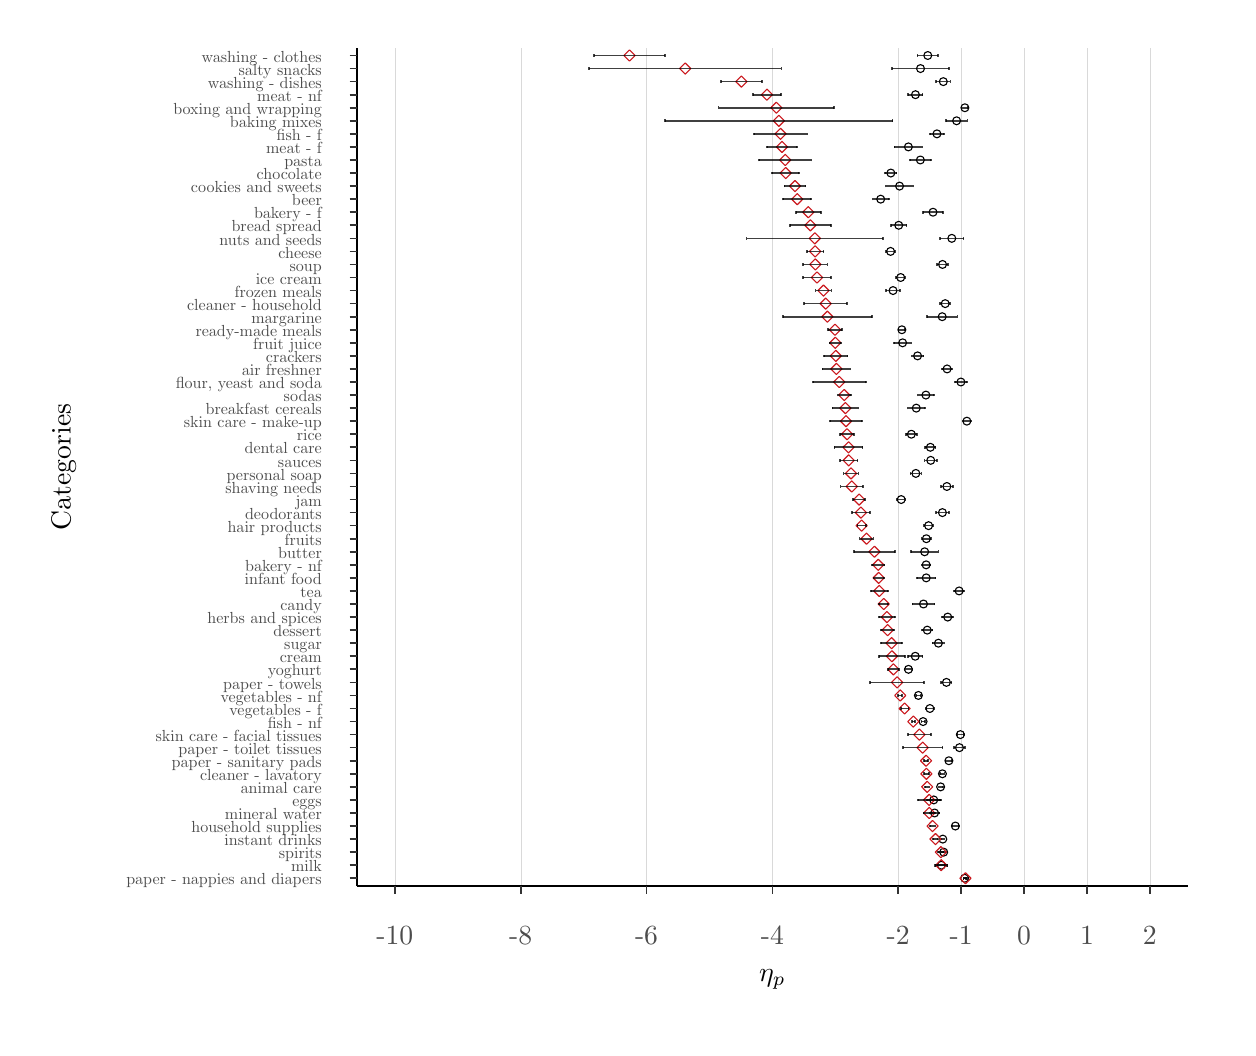
\begin{tikzpicture}[x=1pt,y=1pt]
\definecolor{fillColor}{RGB}{255,255,255}
\path[use as bounding box,fill=fillColor,fill opacity=0.00] (0,0) rectangle (433.62,361.35);
\begin{scope}
\path[clip] (  0.00,  0.00) rectangle (433.62,361.35);
\definecolor{drawColor}{RGB}{255,255,255}
\definecolor{fillColor}{RGB}{255,255,255}

\path[draw=drawColor,line width= 0.6pt,line join=round,line cap=round,fill=fillColor] (  0.00,  0.00) rectangle (433.62,361.35);
\end{scope}
\begin{scope}
\path[clip] (119.04, 51.15) rectangle (419.17,354.12);
\definecolor{drawColor}{RGB}{255,255,255}

\path[draw=drawColor,line width= 0.3pt,line join=round] (155.42, 51.15) --
	(155.42,354.12);

\path[draw=drawColor,line width= 0.3pt,line join=round] (200.89, 51.15) --
	(200.89,354.12);

\path[draw=drawColor,line width= 0.3pt,line join=round] (246.37, 51.15) --
	(246.37,354.12);

\path[draw=drawColor,line width= 0.3pt,line join=round] (291.84, 51.15) --
	(291.84,354.12);

\path[draw=drawColor,line width= 0.3pt,line join=round] (325.95, 51.15) --
	(325.95,354.12);

\path[draw=drawColor,line width= 0.3pt,line join=round] (348.68, 51.15) --
	(348.68,354.12);

\path[draw=drawColor,line width= 0.3pt,line join=round] (371.42, 51.15) --
	(371.42,354.12);

\path[draw=drawColor,line width= 0.3pt,line join=round] (394.16, 51.15) --
	(394.16,354.12);
\definecolor{drawColor}{gray}{0.85}

\path[draw=drawColor,line width= 0.1pt,line join=round] (132.68, 51.15) --
	(132.68,354.12);

\path[draw=drawColor,line width= 0.1pt,line join=round] (178.16, 51.15) --
	(178.16,354.12);

\path[draw=drawColor,line width= 0.1pt,line join=round] (223.63, 51.15) --
	(223.63,354.12);

\path[draw=drawColor,line width= 0.1pt,line join=round] (269.10, 51.15) --
	(269.10,354.12);

\path[draw=drawColor,line width= 0.1pt,line join=round] (314.58, 51.15) --
	(314.58,354.12);

\path[draw=drawColor,line width= 0.1pt,line join=round] (337.31, 51.15) --
	(337.31,354.12);

\path[draw=drawColor,line width= 0.1pt,line join=round] (360.05, 51.15) --
	(360.05,354.12);

\path[draw=drawColor,line width= 0.1pt,line join=round] (382.79, 51.15) --
	(382.79,354.12);

\path[draw=drawColor,line width= 0.1pt,line join=round] (405.52, 51.15) --
	(405.52,354.12);
\definecolor{drawColor}{RGB}{0,0,0}

\path[draw=drawColor,line width= 0.4pt,line join=round,line cap=round] (332.23,238.03) circle (  1.43);

\path[draw=drawColor,line width= 0.4pt,line join=round,line cap=round] (329.89, 87.02) circle (  1.43);

\path[draw=drawColor,line width= 0.4pt,line join=round,line cap=round] (327.14,294.66) circle (  1.43);

\path[draw=drawColor,line width= 0.4pt,line join=round,line cap=round] (324.66,167.24) circle (  1.43);

\path[draw=drawColor,line width= 0.4pt,line join=round,line cap=round] (335.66,327.70) circle (  1.43);

\path[draw=drawColor,line width= 0.4pt,line join=round,line cap=round] (308.23,299.38) circle (  1.43);

\path[draw=drawColor,line width= 0.4pt,line join=round,line cap=round] (338.66,332.41) circle (  1.43);

\path[draw=drawColor,line width= 0.4pt,line join=round,line cap=round] (314.75,289.94) circle (  1.43);

\path[draw=drawColor,line width= 0.4pt,line join=round,line cap=round] (321.09,223.87) circle (  1.43);

\path[draw=drawColor,line width= 0.4pt,line join=round,line cap=round] (324.12,171.96) circle (  1.43);

\path[draw=drawColor,line width= 0.4pt,line join=round,line cap=round] (323.69,153.09) circle (  1.43);

\path[draw=drawColor,line width= 0.4pt,line join=round,line cap=round] (311.80,280.50) circle (  1.43);

\path[draw=drawColor,line width= 0.4pt,line join=round,line cap=round] (311.90,308.82) circle (  1.43);

\path[draw=drawColor,line width= 0.4pt,line join=round,line cap=round] (331.54,261.63) circle (  1.43);

\path[draw=drawColor,line width= 0.4pt,line join=round,line cap=round] (330.54, 91.74) circle (  1.43);

\path[draw=drawColor,line width= 0.4pt,line join=round,line cap=round] (315.05,304.10) circle (  1.43);

\path[draw=drawColor,line width= 0.4pt,line join=round,line cap=round] (321.56,242.75) circle (  1.43);

\path[draw=drawColor,line width= 0.4pt,line join=round,line cap=round] (320.72,134.21) circle (  1.43);

\path[draw=drawColor,line width= 0.4pt,line join=round,line cap=round] (326.19,209.72) circle (  1.43);

\path[draw=drawColor,line width= 0.4pt,line join=round,line cap=round] (330.54,186.12) circle (  1.43);

\path[draw=drawColor,line width= 0.4pt,line join=round,line cap=round] (325.06,143.65) circle (  1.43);

\path[draw=drawColor,line width= 0.4pt,line join=round,line cap=round] (327.40, 82.30) circle (  1.43);

\path[draw=drawColor,line width= 0.4pt,line join=round,line cap=round] (328.56,322.98) circle (  1.43);

\path[draw=drawColor,line width= 0.4pt,line join=round,line cap=round] (323.55,110.61) circle (  1.43);

\path[draw=drawColor,line width= 0.4pt,line join=round,line cap=round] (337.22,233.31) circle (  1.43);

\path[draw=drawColor,line width= 0.4pt,line join=round,line cap=round] (312.69,266.35) circle (  1.43);

\path[draw=drawColor,line width= 0.4pt,line join=round,line cap=round] (316.16,247.47) circle (  1.43);

\path[draw=drawColor,line width= 0.4pt,line join=round,line cap=round] (324.73,176.68) circle (  1.43);

\path[draw=drawColor,line width= 0.4pt,line join=round,line cap=round] (325.54,181.40) circle (  1.43);

\path[draw=drawColor,line width= 0.4pt,line join=round,line cap=round] (332.45,148.37) circle (  1.43);

\path[draw=drawColor,line width= 0.4pt,line join=round,line cap=round] (335.22, 72.86) circle (  1.43);

\path[draw=drawColor,line width= 0.4pt,line join=round,line cap=round] (315.46,271.07) circle (  1.43);

\path[draw=drawColor,line width= 0.4pt,line join=round,line cap=round] (324.69,162.53) circle (  1.43);

\path[draw=drawColor,line width= 0.4pt,line join=round,line cap=round] (330.67, 68.14) circle (  1.43);

\path[draw=drawColor,line width= 0.4pt,line join=round,line cap=round] (315.64,190.84) circle (  1.43);

\path[draw=drawColor,line width= 0.4pt,line join=round,line cap=round] (330.46,256.91) circle (  1.43);

\path[draw=drawColor,line width= 0.4pt,line join=round,line cap=round] (318.25,318.26) circle (  1.43);

\path[draw=drawColor,line width= 0.4pt,line join=round,line cap=round] (320.80,337.13) circle (  1.43);

\path[draw=drawColor,line width= 0.4pt,line join=round,line cap=round] (330.15, 58.70) circle (  1.43);

\path[draw=drawColor,line width= 0.4pt,line join=round,line cap=round] (327.70, 77.58) circle (  1.43);

\path[draw=drawColor,line width= 0.4pt,line join=round,line cap=round] (333.93,285.22) circle (  1.43);

\path[draw=drawColor,line width= 0.4pt,line join=round,line cap=round] (338.57, 53.99) circle (  1.43);

\path[draw=drawColor,line width= 0.4pt,line join=round,line cap=round] (332.88, 96.46) circle (  1.43);

\path[draw=drawColor,line width= 0.4pt,line join=round,line cap=round] (336.70,101.18) circle (  1.43);

\path[draw=drawColor,line width= 0.4pt,line join=round,line cap=round] (331.99,124.77) circle (  1.43);

\path[draw=drawColor,line width= 0.4pt,line join=round,line cap=round] (322.57,313.54) circle (  1.43);

\path[draw=drawColor,line width= 0.4pt,line join=round,line cap=round] (320.94,200.28) circle (  1.43);

\path[draw=drawColor,line width= 0.4pt,line join=round,line cap=round] (315.89,252.19) circle (  1.43);

\path[draw=drawColor,line width= 0.4pt,line join=round,line cap=round] (319.31,214.44) circle (  1.43);

\path[draw=drawColor,line width= 0.4pt,line join=round,line cap=round] (322.62,346.57) circle (  1.43);

\path[draw=drawColor,line width= 0.4pt,line join=round,line cap=round] (326.32,205.00) circle (  1.43);

\path[draw=drawColor,line width= 0.4pt,line join=round,line cap=round] (332.15,195.56) circle (  1.43);

\path[draw=drawColor,line width= 0.4pt,line join=round,line cap=round] (337.03,105.90) circle (  1.43);

\path[draw=drawColor,line width= 0.4pt,line join=round,line cap=round] (339.37,219.16) circle (  1.43);

\path[draw=drawColor,line width= 0.4pt,line join=round,line cap=round] (324.57,228.59) circle (  1.43);

\path[draw=drawColor,line width= 0.4pt,line join=round,line cap=round] (330.58,275.79) circle (  1.43);

\path[draw=drawColor,line width= 0.4pt,line join=round,line cap=round] (331.00, 63.42) circle (  1.43);

\path[draw=drawColor,line width= 0.4pt,line join=round,line cap=round] (329.09,138.93) circle (  1.43);

\path[draw=drawColor,line width= 0.4pt,line join=round,line cap=round] (336.58,157.81) circle (  1.43);

\path[draw=drawColor,line width= 0.4pt,line join=round,line cap=round] (326.02,115.33) circle (  1.43);

\path[draw=drawColor,line width= 0.4pt,line join=round,line cap=round] (321.86,120.05) circle (  1.43);

\path[draw=drawColor,line width= 0.4pt,line join=round,line cap=round] (325.25,351.29) circle (  1.43);

\path[draw=drawColor,line width= 0.4pt,line join=round,line cap=round] (330.86,341.85) circle (  1.43);

\path[draw=drawColor,line width= 0.4pt,line join=round,line cap=round] (318.27,129.49) circle (  1.43);
\definecolor{drawColor}{RGB}{0,0,0}

\path[draw=drawColor,draw opacity=0.75,line width= 0.6pt,line join=round] (334.10,237.56) --
	(334.10,238.50);

\path[draw=drawColor,draw opacity=0.75,line width= 0.6pt,line join=round] (334.10,238.03) --
	(330.36,238.03);

\path[draw=drawColor,draw opacity=0.75,line width= 0.6pt,line join=round] (330.36,237.56) --
	(330.36,238.50);

\path[draw=drawColor,draw opacity=0.75,line width= 0.6pt,line join=round] (330.65, 86.55) --
	(330.65, 87.49);

\path[draw=drawColor,draw opacity=0.75,line width= 0.6pt,line join=round] (330.65, 87.02) --
	(329.13, 87.02);

\path[draw=drawColor,draw opacity=0.75,line width= 0.6pt,line join=round] (329.13, 86.55) --
	(329.13, 87.49);

\path[draw=drawColor,draw opacity=0.75,line width= 0.6pt,line join=round] (330.80,294.19) --
	(330.80,295.13);

\path[draw=drawColor,draw opacity=0.75,line width= 0.6pt,line join=round] (330.80,294.66) --
	(323.49,294.66);

\path[draw=drawColor,draw opacity=0.75,line width= 0.6pt,line join=round] (323.49,294.19) --
	(323.49,295.13);

\path[draw=drawColor,draw opacity=0.75,line width= 0.6pt,line join=round] (326.29,166.77) --
	(326.29,167.72);

\path[draw=drawColor,draw opacity=0.75,line width= 0.6pt,line join=round] (326.29,167.24) --
	(323.03,167.24);

\path[draw=drawColor,draw opacity=0.75,line width= 0.6pt,line join=round] (323.03,166.77) --
	(323.03,167.72);

\path[draw=drawColor,draw opacity=0.75,line width= 0.6pt,line join=round] (339.59,327.22) --
	(339.59,328.17);

\path[draw=drawColor,draw opacity=0.75,line width= 0.6pt,line join=round] (339.59,327.70) --
	(331.72,327.70);

\path[draw=drawColor,draw opacity=0.75,line width= 0.6pt,line join=round] (331.72,327.22) --
	(331.72,328.17);

\path[draw=drawColor,draw opacity=0.75,line width= 0.6pt,line join=round] (311.16,298.91) --
	(311.16,299.85);

\path[draw=drawColor,draw opacity=0.75,line width= 0.6pt,line join=round] (311.16,299.38) --
	(305.31,299.38);

\path[draw=drawColor,draw opacity=0.75,line width= 0.6pt,line join=round] (305.31,298.91) --
	(305.31,299.85);

\path[draw=drawColor,draw opacity=0.75,line width= 0.6pt,line join=round] (339.84,331.94) --
	(339.84,332.89);

\path[draw=drawColor,draw opacity=0.75,line width= 0.6pt,line join=round] (339.84,332.41) --
	(337.49,332.41);

\path[draw=drawColor,draw opacity=0.75,line width= 0.6pt,line join=round] (337.49,331.94) --
	(337.49,332.89);

\path[draw=drawColor,draw opacity=0.75,line width= 0.6pt,line join=round] (317.61,289.47) --
	(317.61,290.41);

\path[draw=drawColor,draw opacity=0.75,line width= 0.6pt,line join=round] (317.61,289.94) --
	(311.89,289.94);

\path[draw=drawColor,draw opacity=0.75,line width= 0.6pt,line join=round] (311.89,289.47) --
	(311.89,290.41);

\path[draw=drawColor,draw opacity=0.75,line width= 0.6pt,line join=round] (324.20,223.40) --
	(324.20,224.35);

\path[draw=drawColor,draw opacity=0.75,line width= 0.6pt,line join=round] (324.20,223.87) --
	(317.97,223.87);

\path[draw=drawColor,draw opacity=0.75,line width= 0.6pt,line join=round] (317.97,223.40) --
	(317.97,224.35);

\path[draw=drawColor,draw opacity=0.75,line width= 0.6pt,line join=round] (329.12,171.49) --
	(329.12,172.44);

\path[draw=drawColor,draw opacity=0.75,line width= 0.6pt,line join=round] (329.12,171.96) --
	(319.12,171.96);

\path[draw=drawColor,draw opacity=0.75,line width= 0.6pt,line join=round] (319.12,171.49) --
	(319.12,172.44);

\path[draw=drawColor,draw opacity=0.75,line width= 0.6pt,line join=round] (327.70,152.62) --
	(327.70,153.56);

\path[draw=drawColor,draw opacity=0.75,line width= 0.6pt,line join=round] (327.70,153.09) --
	(319.68,153.09);

\path[draw=drawColor,draw opacity=0.75,line width= 0.6pt,line join=round] (319.68,152.62) --
	(319.68,153.56);

\path[draw=drawColor,draw opacity=0.75,line width= 0.6pt,line join=round] (313.35,280.03) --
	(313.35,280.98);

\path[draw=drawColor,draw opacity=0.75,line width= 0.6pt,line join=round] (313.35,280.50) --
	(310.25,280.50);

\path[draw=drawColor,draw opacity=0.75,line width= 0.6pt,line join=round] (310.25,280.03) --
	(310.25,280.98);

\path[draw=drawColor,draw opacity=0.75,line width= 0.6pt,line join=round] (313.95,308.35) --
	(313.95,309.29);

\path[draw=drawColor,draw opacity=0.75,line width= 0.6pt,line join=round] (313.95,308.82) --
	(309.84,308.82);

\path[draw=drawColor,draw opacity=0.75,line width= 0.6pt,line join=round] (309.84,308.35) --
	(309.84,309.29);

\path[draw=drawColor,draw opacity=0.75,line width= 0.6pt,line join=round] (333.35,261.16) --
	(333.35,262.10);

\path[draw=drawColor,draw opacity=0.75,line width= 0.6pt,line join=round] (333.35,261.63) --
	(329.72,261.63);

\path[draw=drawColor,draw opacity=0.75,line width= 0.6pt,line join=round] (329.72,261.16) --
	(329.72,262.10);

\path[draw=drawColor,draw opacity=0.75,line width= 0.6pt,line join=round] (331.29, 91.27) --
	(331.29, 92.21);

\path[draw=drawColor,draw opacity=0.75,line width= 0.6pt,line join=round] (331.29, 91.74) --
	(329.78, 91.74);

\path[draw=drawColor,draw opacity=0.75,line width= 0.6pt,line join=round] (329.78, 91.27) --
	(329.78, 92.21);

\path[draw=drawColor,draw opacity=0.75,line width= 0.6pt,line join=round] (320.08,303.63) --
	(320.08,304.57);

\path[draw=drawColor,draw opacity=0.75,line width= 0.6pt,line join=round] (320.08,304.10) --
	(310.01,304.10);

\path[draw=drawColor,draw opacity=0.75,line width= 0.6pt,line join=round] (310.01,303.63) --
	(310.01,304.57);

\path[draw=drawColor,draw opacity=0.75,line width= 0.6pt,line join=round] (323.74,242.28) --
	(323.74,243.22);

\path[draw=drawColor,draw opacity=0.75,line width= 0.6pt,line join=round] (323.74,242.75) --
	(319.38,242.75);

\path[draw=drawColor,draw opacity=0.75,line width= 0.6pt,line join=round] (319.38,242.28) --
	(319.38,243.22);

\path[draw=drawColor,draw opacity=0.75,line width= 0.6pt,line join=round] (323.40,133.74) --
	(323.40,134.68);

\path[draw=drawColor,draw opacity=0.75,line width= 0.6pt,line join=round] (323.40,134.21) --
	(318.04,134.21);

\path[draw=drawColor,draw opacity=0.75,line width= 0.6pt,line join=round] (318.04,133.74) --
	(318.04,134.68);

\path[draw=drawColor,draw opacity=0.75,line width= 0.6pt,line join=round] (328.09,209.25) --
	(328.09,210.19);

\path[draw=drawColor,draw opacity=0.75,line width= 0.6pt,line join=round] (328.09,209.72) --
	(324.28,209.72);

\path[draw=drawColor,draw opacity=0.75,line width= 0.6pt,line join=round] (324.28,209.25) --
	(324.28,210.19);

\path[draw=drawColor,draw opacity=0.75,line width= 0.6pt,line join=round] (332.93,185.65) --
	(332.93,186.59);

\path[draw=drawColor,draw opacity=0.75,line width= 0.6pt,line join=round] (332.93,186.12) --
	(328.15,186.12);

\path[draw=drawColor,draw opacity=0.75,line width= 0.6pt,line join=round] (328.15,185.65) --
	(328.15,186.59);

\path[draw=drawColor,draw opacity=0.75,line width= 0.6pt,line join=round] (327.01,143.18) --
	(327.01,144.12);

\path[draw=drawColor,draw opacity=0.75,line width= 0.6pt,line join=round] (327.01,143.65) --
	(323.11,143.65);

\path[draw=drawColor,draw opacity=0.75,line width= 0.6pt,line join=round] (323.11,143.18) --
	(323.11,144.12);

\path[draw=drawColor,draw opacity=0.75,line width= 0.6pt,line join=round] (329.93, 81.83) --
	(329.93, 82.77);

\path[draw=drawColor,draw opacity=0.75,line width= 0.6pt,line join=round] (329.93, 82.30) --
	(324.87, 82.30);

\path[draw=drawColor,draw opacity=0.75,line width= 0.6pt,line join=round] (324.87, 81.83) --
	(324.87, 82.77);

\path[draw=drawColor,draw opacity=0.75,line width= 0.6pt,line join=round] (331.09,322.50) --
	(331.09,323.45);

\path[draw=drawColor,draw opacity=0.75,line width= 0.6pt,line join=round] (331.09,322.98) --
	(326.03,322.98);

\path[draw=drawColor,draw opacity=0.75,line width= 0.6pt,line join=round] (326.03,322.50) --
	(326.03,323.45);

\path[draw=drawColor,draw opacity=0.75,line width= 0.6pt,line join=round] (324.16,110.14) --
	(324.16,111.09);

\path[draw=drawColor,draw opacity=0.75,line width= 0.6pt,line join=round] (324.16,110.61) --
	(322.95,110.61);

\path[draw=drawColor,draw opacity=0.75,line width= 0.6pt,line join=round] (322.95,110.14) --
	(322.95,111.09);

\path[draw=drawColor,draw opacity=0.75,line width= 0.6pt,line join=round] (339.41,232.84) --
	(339.41,233.78);

\path[draw=drawColor,draw opacity=0.75,line width= 0.6pt,line join=round] (339.41,233.31) --
	(335.02,233.31);

\path[draw=drawColor,draw opacity=0.75,line width= 0.6pt,line join=round] (335.02,232.84) --
	(335.02,233.78);

\path[draw=drawColor,draw opacity=0.75,line width= 0.6pt,line join=round] (315.17,265.87) --
	(315.17,266.82);

\path[draw=drawColor,draw opacity=0.75,line width= 0.6pt,line join=round] (315.17,266.35) --
	(310.21,266.35);

\path[draw=drawColor,draw opacity=0.75,line width= 0.6pt,line join=round] (310.21,265.87) --
	(310.21,266.82);

\path[draw=drawColor,draw opacity=0.75,line width= 0.6pt,line join=round] (319.32,247.00) --
	(319.32,247.94);

\path[draw=drawColor,draw opacity=0.75,line width= 0.6pt,line join=round] (319.32,247.47) --
	(312.99,247.47);

\path[draw=drawColor,draw opacity=0.75,line width= 0.6pt,line join=round] (312.99,247.00) --
	(312.99,247.94);

\path[draw=drawColor,draw opacity=0.75,line width= 0.6pt,line join=round] (326.47,176.21) --
	(326.47,177.15);

\path[draw=drawColor,draw opacity=0.75,line width= 0.6pt,line join=round] (326.47,176.68) --
	(322.98,176.68);

\path[draw=drawColor,draw opacity=0.75,line width= 0.6pt,line join=round] (322.98,176.21) --
	(322.98,177.15);

\path[draw=drawColor,draw opacity=0.75,line width= 0.6pt,line join=round] (327.22,180.93) --
	(327.22,181.87);

\path[draw=drawColor,draw opacity=0.75,line width= 0.6pt,line join=round] (327.22,181.40) --
	(323.87,181.40);

\path[draw=drawColor,draw opacity=0.75,line width= 0.6pt,line join=round] (323.87,180.93) --
	(323.87,181.87);

\path[draw=drawColor,draw opacity=0.75,line width= 0.6pt,line join=round] (334.47,147.90) --
	(334.47,148.84);

\path[draw=drawColor,draw opacity=0.75,line width= 0.6pt,line join=round] (334.47,148.37) --
	(330.42,148.37);

\path[draw=drawColor,draw opacity=0.75,line width= 0.6pt,line join=round] (330.42,147.90) --
	(330.42,148.84);

\path[draw=drawColor,draw opacity=0.75,line width= 0.6pt,line join=round] (336.42, 72.39) --
	(336.42, 73.33);

\path[draw=drawColor,draw opacity=0.75,line width= 0.6pt,line join=round] (336.42, 72.86) --
	(334.01, 72.86);

\path[draw=drawColor,draw opacity=0.75,line width= 0.6pt,line join=round] (334.01, 72.39) --
	(334.01, 73.33);

\path[draw=drawColor,draw opacity=0.75,line width= 0.6pt,line join=round] (317.12,270.59) --
	(317.12,271.54);

\path[draw=drawColor,draw opacity=0.75,line width= 0.6pt,line join=round] (317.12,271.07) --
	(313.80,271.07);

\path[draw=drawColor,draw opacity=0.75,line width= 0.6pt,line join=round] (313.80,270.59) --
	(313.80,271.54);

\path[draw=drawColor,draw opacity=0.75,line width= 0.6pt,line join=round] (328.05,162.05) --
	(328.05,163.00);

\path[draw=drawColor,draw opacity=0.75,line width= 0.6pt,line join=round] (328.05,162.53) --
	(321.34,162.53);

\path[draw=drawColor,draw opacity=0.75,line width= 0.6pt,line join=round] (321.34,162.05) --
	(321.34,163.00);

\path[draw=drawColor,draw opacity=0.75,line width= 0.6pt,line join=round] (331.24, 67.67) --
	(331.24, 68.61);

\path[draw=drawColor,draw opacity=0.75,line width= 0.6pt,line join=round] (331.24, 68.14) --
	(330.10, 68.14);

\path[draw=drawColor,draw opacity=0.75,line width= 0.6pt,line join=round] (330.10, 67.67) --
	(330.10, 68.61);

\path[draw=drawColor,draw opacity=0.75,line width= 0.6pt,line join=round] (317.16,190.37) --
	(317.16,191.31);

\path[draw=drawColor,draw opacity=0.75,line width= 0.6pt,line join=round] (317.16,190.84) --
	(314.13,190.84);

\path[draw=drawColor,draw opacity=0.75,line width= 0.6pt,line join=round] (314.13,190.37) --
	(314.13,191.31);

\path[draw=drawColor,draw opacity=0.75,line width= 0.6pt,line join=round] (335.95,256.44) --
	(335.95,257.38);

\path[draw=drawColor,draw opacity=0.75,line width= 0.6pt,line join=round] (335.95,256.91) --
	(324.97,256.91);

\path[draw=drawColor,draw opacity=0.75,line width= 0.6pt,line join=round] (324.97,256.44) --
	(324.97,257.38);

\path[draw=drawColor,draw opacity=0.75,line width= 0.6pt,line join=round] (323.31,317.79) --
	(323.31,318.73);

\path[draw=drawColor,draw opacity=0.75,line width= 0.6pt,line join=round] (323.31,318.26) --
	(313.19,318.26);

\path[draw=drawColor,draw opacity=0.75,line width= 0.6pt,line join=round] (313.19,317.79) --
	(313.19,318.73);

\path[draw=drawColor,draw opacity=0.75,line width= 0.6pt,line join=round] (323.40,336.66) --
	(323.40,337.61);

\path[draw=drawColor,draw opacity=0.75,line width= 0.6pt,line join=round] (323.40,337.13) --
	(318.19,337.13);

\path[draw=drawColor,draw opacity=0.75,line width= 0.6pt,line join=round] (318.19,336.66) --
	(318.19,337.61);

\path[draw=drawColor,draw opacity=0.75,line width= 0.6pt,line join=round] (332.08, 58.23) --
	(332.08, 59.18);

\path[draw=drawColor,draw opacity=0.75,line width= 0.6pt,line join=round] (332.08, 58.70) --
	(328.22, 58.70);

\path[draw=drawColor,draw opacity=0.75,line width= 0.6pt,line join=round] (328.22, 58.23) --
	(328.22, 59.18);

\path[draw=drawColor,draw opacity=0.75,line width= 0.6pt,line join=round] (329.52, 77.11) --
	(329.52, 78.05);

\path[draw=drawColor,draw opacity=0.75,line width= 0.6pt,line join=round] (329.52, 77.58) --
	(325.88, 77.58);

\path[draw=drawColor,draw opacity=0.75,line width= 0.6pt,line join=round] (325.88, 77.11) --
	(325.88, 78.05);

\path[draw=drawColor,draw opacity=0.75,line width= 0.6pt,line join=round] (338.20,284.75) --
	(338.20,285.70);

\path[draw=drawColor,draw opacity=0.75,line width= 0.6pt,line join=round] (338.20,285.22) --
	(329.66,285.22);

\path[draw=drawColor,draw opacity=0.75,line width= 0.6pt,line join=round] (329.66,284.75) --
	(329.66,285.70);

\path[draw=drawColor,draw opacity=0.75,line width= 0.6pt,line join=round] (338.97, 53.51) --
	(338.97, 54.46);

\path[draw=drawColor,draw opacity=0.75,line width= 0.6pt,line join=round] (338.97, 53.99) --
	(338.17, 53.99);

\path[draw=drawColor,draw opacity=0.75,line width= 0.6pt,line join=round] (338.17, 53.51) --
	(338.17, 54.46);

\path[draw=drawColor,draw opacity=0.75,line width= 0.6pt,line join=round] (334.11, 95.99) --
	(334.11, 96.93);

\path[draw=drawColor,draw opacity=0.75,line width= 0.6pt,line join=round] (334.11, 96.46) --
	(331.65, 96.46);

\path[draw=drawColor,draw opacity=0.75,line width= 0.6pt,line join=round] (331.65, 95.99) --
	(331.65, 96.93);

\path[draw=drawColor,draw opacity=0.75,line width= 0.6pt,line join=round] (338.61,100.70) --
	(338.61,101.65);

\path[draw=drawColor,draw opacity=0.75,line width= 0.6pt,line join=round] (338.61,101.18) --
	(334.79,101.18);

\path[draw=drawColor,draw opacity=0.75,line width= 0.6pt,line join=round] (334.79,100.70) --
	(334.79,101.65);

\path[draw=drawColor,draw opacity=0.75,line width= 0.6pt,line join=round] (333.86,124.30) --
	(333.86,125.24);

\path[draw=drawColor,draw opacity=0.75,line width= 0.6pt,line join=round] (333.86,124.77) --
	(330.11,124.77);

\path[draw=drawColor,draw opacity=0.75,line width= 0.6pt,line join=round] (330.11,124.30) --
	(330.11,125.24);

\path[draw=drawColor,draw opacity=0.75,line width= 0.6pt,line join=round] (326.33,313.07) --
	(326.33,314.01);

\path[draw=drawColor,draw opacity=0.75,line width= 0.6pt,line join=round] (326.33,313.54) --
	(318.81,313.54);

\path[draw=drawColor,draw opacity=0.75,line width= 0.6pt,line join=round] (318.81,313.07) --
	(318.81,314.01);

\path[draw=drawColor,draw opacity=0.75,line width= 0.6pt,line join=round] (322.92,199.81) --
	(322.92,200.75);

\path[draw=drawColor,draw opacity=0.75,line width= 0.6pt,line join=round] (322.92,200.28) --
	(318.96,200.28);

\path[draw=drawColor,draw opacity=0.75,line width= 0.6pt,line join=round] (318.96,199.81) --
	(318.96,200.75);

\path[draw=drawColor,draw opacity=0.75,line width= 0.6pt,line join=round] (317.12,251.72) --
	(317.12,252.66);

\path[draw=drawColor,draw opacity=0.75,line width= 0.6pt,line join=round] (317.12,252.19) --
	(314.66,252.19);

\path[draw=drawColor,draw opacity=0.75,line width= 0.6pt,line join=round] (314.66,251.72) --
	(314.66,252.66);

\path[draw=drawColor,draw opacity=0.75,line width= 0.6pt,line join=round] (321.34,213.96) --
	(321.34,214.91);

\path[draw=drawColor,draw opacity=0.75,line width= 0.6pt,line join=round] (321.34,214.44) --
	(317.28,214.44);

\path[draw=drawColor,draw opacity=0.75,line width= 0.6pt,line join=round] (317.28,213.96) --
	(317.28,214.91);

\path[draw=drawColor,draw opacity=0.75,line width= 0.6pt,line join=round] (333.02,346.10) --
	(333.02,347.04);

\path[draw=drawColor,draw opacity=0.75,line width= 0.6pt,line join=round] (333.02,346.57) --
	(312.22,346.57);

\path[draw=drawColor,draw opacity=0.75,line width= 0.6pt,line join=round] (312.22,346.10) --
	(312.22,347.04);

\path[draw=drawColor,draw opacity=0.75,line width= 0.6pt,line join=round] (328.52,204.53) --
	(328.52,205.47);

\path[draw=drawColor,draw opacity=0.75,line width= 0.6pt,line join=round] (328.52,205.00) --
	(324.12,205.00);

\path[draw=drawColor,draw opacity=0.75,line width= 0.6pt,line join=round] (324.12,204.53) --
	(324.12,205.47);

\path[draw=drawColor,draw opacity=0.75,line width= 0.6pt,line join=round] (334.39,195.09) --
	(334.39,196.03);

\path[draw=drawColor,draw opacity=0.75,line width= 0.6pt,line join=round] (334.39,195.56) --
	(329.91,195.56);

\path[draw=drawColor,draw opacity=0.75,line width= 0.6pt,line join=round] (329.91,195.09) --
	(329.91,196.03);

\path[draw=drawColor,draw opacity=0.75,line width= 0.6pt,line join=round] (338.25,105.42) --
	(338.25,106.37);

\path[draw=drawColor,draw opacity=0.75,line width= 0.6pt,line join=round] (338.25,105.90) --
	(335.82,105.90);

\path[draw=drawColor,draw opacity=0.75,line width= 0.6pt,line join=round] (335.82,105.42) --
	(335.82,106.37);

\path[draw=drawColor,draw opacity=0.75,line width= 0.6pt,line join=round] (340.88,218.68) --
	(340.88,219.63);

\path[draw=drawColor,draw opacity=0.75,line width= 0.6pt,line join=round] (340.88,219.16) --
	(337.87,219.16);

\path[draw=drawColor,draw opacity=0.75,line width= 0.6pt,line join=round] (337.87,218.68) --
	(337.87,219.63);

\path[draw=drawColor,draw opacity=0.75,line width= 0.6pt,line join=round] (327.56,228.12) --
	(327.56,229.07);

\path[draw=drawColor,draw opacity=0.75,line width= 0.6pt,line join=round] (327.56,228.59) --
	(321.57,228.59);

\path[draw=drawColor,draw opacity=0.75,line width= 0.6pt,line join=round] (321.57,228.12) --
	(321.57,229.07);

\path[draw=drawColor,draw opacity=0.75,line width= 0.6pt,line join=round] (332.55,275.31) --
	(332.55,276.26);

\path[draw=drawColor,draw opacity=0.75,line width= 0.6pt,line join=round] (332.55,275.79) --
	(328.61,275.79);

\path[draw=drawColor,draw opacity=0.75,line width= 0.6pt,line join=round] (328.61,275.31) --
	(328.61,276.26);

\path[draw=drawColor,draw opacity=0.75,line width= 0.6pt,line join=round] (331.79, 62.95) --
	(331.79, 63.90);

\path[draw=drawColor,draw opacity=0.75,line width= 0.6pt,line join=round] (331.79, 63.42) --
	(330.22, 63.42);

\path[draw=drawColor,draw opacity=0.75,line width= 0.6pt,line join=round] (330.22, 62.95) --
	(330.22, 63.90);

\path[draw=drawColor,draw opacity=0.75,line width= 0.6pt,line join=round] (331.28,138.46) --
	(331.28,139.40);

\path[draw=drawColor,draw opacity=0.75,line width= 0.6pt,line join=round] (331.28,138.93) --
	(326.91,138.93);

\path[draw=drawColor,draw opacity=0.75,line width= 0.6pt,line join=round] (326.91,138.46) --
	(326.91,139.40);

\path[draw=drawColor,draw opacity=0.75,line width= 0.6pt,line join=round] (338.42,157.33) --
	(338.42,158.28);

\path[draw=drawColor,draw opacity=0.75,line width= 0.6pt,line join=round] (338.42,157.81) --
	(334.73,157.81);

\path[draw=drawColor,draw opacity=0.75,line width= 0.6pt,line join=round] (334.73,157.33) --
	(334.73,158.28);

\path[draw=drawColor,draw opacity=0.75,line width= 0.6pt,line join=round] (327.52,114.86) --
	(327.52,115.81);

\path[draw=drawColor,draw opacity=0.75,line width= 0.6pt,line join=round] (327.52,115.33) --
	(324.52,115.33);

\path[draw=drawColor,draw opacity=0.75,line width= 0.6pt,line join=round] (324.52,114.86) --
	(324.52,115.81);

\path[draw=drawColor,draw opacity=0.75,line width= 0.6pt,line join=round] (322.82,119.58) --
	(322.82,120.53);

\path[draw=drawColor,draw opacity=0.75,line width= 0.6pt,line join=round] (322.82,120.05) --
	(320.91,120.05);

\path[draw=drawColor,draw opacity=0.75,line width= 0.6pt,line join=round] (320.91,119.58) --
	(320.91,120.53);

\path[draw=drawColor,draw opacity=0.75,line width= 0.6pt,line join=round] (328.99,350.82) --
	(328.99,351.76);

\path[draw=drawColor,draw opacity=0.75,line width= 0.6pt,line join=round] (328.99,351.29) --
	(321.52,351.29);

\path[draw=drawColor,draw opacity=0.75,line width= 0.6pt,line join=round] (321.52,350.82) --
	(321.52,351.76);

\path[draw=drawColor,draw opacity=0.75,line width= 0.6pt,line join=round] (333.42,341.38) --
	(333.42,342.33);

\path[draw=drawColor,draw opacity=0.75,line width= 0.6pt,line join=round] (333.42,341.85) --
	(328.30,341.85);

\path[draw=drawColor,draw opacity=0.75,line width= 0.6pt,line join=round] (328.30,341.38) --
	(328.30,342.33);

\path[draw=drawColor,draw opacity=0.75,line width= 0.6pt,line join=round] (319.69,129.02) --
	(319.69,129.96);

\path[draw=drawColor,draw opacity=0.75,line width= 0.6pt,line join=round] (319.69,129.49) --
	(316.84,129.49);

\path[draw=drawColor,draw opacity=0.75,line width= 0.6pt,line join=round] (316.84,129.02) --
	(316.84,129.96);
\definecolor{drawColor}{RGB}{203,24,29}

\path[draw=drawColor,line width= 0.4pt,line join=round,line cap=round] (290.22,238.03) --
	(292.24,240.05) --
	(294.25,238.03) --
	(292.24,236.01) --
	cycle;

\path[draw=drawColor,line width= 0.4pt,line join=round,line cap=round] (323.03, 87.02) --
	(325.04, 89.04) --
	(327.06, 87.02) --
	(325.04, 85.00) --
	cycle;

\path[draw=drawColor,line width= 0.4pt,line join=round,line cap=round] (280.05,294.66) --
	(282.07,296.68) --
	(284.09,294.66) --
	(282.07,292.64) --
	cycle;

\path[draw=drawColor,line width= 0.4pt,line join=round,line cap=round] (305.34,167.24) --
	(307.36,169.26) --
	(309.38,167.24) --
	(307.36,165.23) --
	cycle;

\path[draw=drawColor,line width= 0.4pt,line join=round,line cap=round] (269.42,327.70) --
	(271.44,329.71) --
	(273.46,327.70) --
	(271.44,325.68) --
	cycle;

\path[draw=drawColor,line width= 0.4pt,line join=round,line cap=round] (276.06,299.38) --
	(278.08,301.40) --
	(280.09,299.38) --
	(278.08,297.36) --
	cycle;

\path[draw=drawColor,line width= 0.4pt,line join=round,line cap=round] (268.52,332.41) --
	(270.53,334.43) --
	(272.55,332.41) --
	(270.53,330.40) --
	cycle;

\path[draw=drawColor,line width= 0.4pt,line join=round,line cap=round] (280.81,289.94) --
	(282.83,291.96) --
	(284.84,289.94) --
	(282.83,287.92) --
	cycle;

\path[draw=drawColor,line width= 0.4pt,line join=round,line cap=round] (293.47,223.87) --
	(295.49,225.89) --
	(297.51,223.87) --
	(295.49,221.86) --
	cycle;

\path[draw=drawColor,line width= 0.4pt,line join=round,line cap=round] (303.95,171.96) --
	(305.97,173.98) --
	(307.99,171.96) --
	(305.97,169.95) --
	cycle;

\path[draw=drawColor,line width= 0.4pt,line join=round,line cap=round] (307.31,153.09) --
	(309.33,155.10) --
	(311.35,153.09) --
	(309.33,151.07) --
	cycle;

\path[draw=drawColor,line width= 0.4pt,line join=round,line cap=round] (282.53,280.50) --
	(284.55,282.52) --
	(286.57,280.50) --
	(284.55,278.49) --
	cycle;

\path[draw=drawColor,line width= 0.4pt,line join=round,line cap=round] (271.89,308.82) --
	(273.91,310.84) --
	(275.93,308.82) --
	(273.91,306.80) --
	cycle;

\path[draw=drawColor,line width= 0.4pt,line join=round,line cap=round] (286.34,261.63) --
	(288.36,263.65) --
	(290.38,261.63) --
	(288.36,259.61) --
	cycle;

\path[draw=drawColor,line width= 0.4pt,line join=round,line cap=round] (322.73, 91.74) --
	(324.75, 93.76) --
	(326.77, 91.74) --
	(324.75, 89.72) --
	cycle;

\path[draw=drawColor,line width= 0.4pt,line join=round,line cap=round] (275.26,304.10) --
	(277.27,306.12) --
	(279.29,304.10) --
	(277.27,302.08) --
	cycle;

\path[draw=drawColor,line width= 0.4pt,line join=round,line cap=round] (289.98,242.75) --
	(292.00,244.77) --
	(294.02,242.75) --
	(292.00,240.73) --
	cycle;

\path[draw=drawColor,line width= 0.4pt,line join=round,line cap=round] (310.27,134.21) --
	(312.29,136.23) --
	(314.31,134.21) --
	(312.29,132.19) --
	cycle;

\path[draw=drawColor,line width= 0.4pt,line join=round,line cap=round] (294.61,209.72) --
	(296.63,211.73) --
	(298.64,209.72) --
	(296.63,207.70) --
	cycle;

\path[draw=drawColor,line width= 0.4pt,line join=round,line cap=round] (299.08,186.12) --
	(301.10,188.14) --
	(303.12,186.12) --
	(301.10,184.10) --
	cycle;

\path[draw=drawColor,line width= 0.4pt,line join=round,line cap=round] (308.71,143.65) --
	(310.73,145.67) --
	(312.75,143.65) --
	(310.73,141.63) --
	cycle;

\path[draw=drawColor,line width= 0.4pt,line join=round,line cap=round] (323.73, 82.30) --
	(325.75, 84.32) --
	(327.77, 82.30) --
	(325.75, 80.28) --
	cycle;

\path[draw=drawColor,line width= 0.4pt,line join=round,line cap=round] (270.02,322.98) --
	(272.04,324.99) --
	(274.06,322.98) --
	(272.04,320.96) --
	cycle;

\path[draw=drawColor,line width= 0.4pt,line join=round,line cap=round] (318.01,110.61) --
	(320.03,112.63) --
	(322.04,110.61) --
	(320.03,108.60) --
	cycle;

\path[draw=drawColor,line width= 0.4pt,line join=round,line cap=round] (291.23,233.31) --
	(293.25,235.33) --
	(295.27,233.31) --
	(293.25,231.30) --
	cycle;

\path[draw=drawColor,line width= 0.4pt,line join=round,line cap=round] (285.55,266.35) --
	(287.57,268.36) --
	(289.58,266.35) --
	(287.57,264.33) --
	cycle;

\path[draw=drawColor,line width= 0.4pt,line join=round,line cap=round] (289.81,247.47) --
	(291.82,249.49) --
	(293.84,247.47) --
	(291.82,245.45) --
	cycle;

\path[draw=drawColor,line width= 0.4pt,line join=round,line cap=round] (301.10,176.68) --
	(303.11,178.70) --
	(305.13,176.68) --
	(303.11,174.67) --
	cycle;

\path[draw=drawColor,line width= 0.4pt,line join=round,line cap=round] (299.33,181.40) --
	(301.35,183.42) --
	(303.37,181.40) --
	(301.35,179.38) --
	cycle;

\path[draw=drawColor,line width= 0.4pt,line join=round,line cap=round] (308.47,148.37) --
	(310.49,150.39) --
	(312.51,148.37) --
	(310.49,146.35) --
	cycle;

\path[draw=drawColor,line width= 0.4pt,line join=round,line cap=round] (324.97, 72.86) --
	(326.98, 74.88) --
	(329.00, 72.86) --
	(326.98, 70.84) --
	cycle;

\path[draw=drawColor,line width= 0.4pt,line join=round,line cap=round] (283.19,271.07) --
	(285.21,273.08) --
	(287.23,271.07) --
	(285.21,269.05) --
	cycle;

\path[draw=drawColor,line width= 0.4pt,line join=round,line cap=round] (305.50,162.53) --
	(307.52,164.54) --
	(309.54,162.53) --
	(307.52,160.51) --
	cycle;

\path[draw=drawColor,line width= 0.4pt,line join=round,line cap=round] (326.01, 68.14) --
	(328.03, 70.16) --
	(330.05, 68.14) --
	(328.03, 66.12) --
	cycle;

\path[draw=drawColor,line width= 0.4pt,line join=round,line cap=round] (298.42,190.84) --
	(300.44,192.86) --
	(302.46,190.84) --
	(300.44,188.82) --
	cycle;

\path[draw=drawColor,line width= 0.4pt,line join=round,line cap=round] (286.96,256.91) --
	(288.97,258.93) --
	(290.99,256.91) --
	(288.97,254.89) --
	cycle;

\path[draw=drawColor,line width= 0.4pt,line join=round,line cap=round] (270.56,318.26) --
	(272.58,320.28) --
	(274.60,318.26) --
	(272.58,316.24) --
	cycle;

\path[draw=drawColor,line width= 0.4pt,line join=round,line cap=round] (265.12,337.13) --
	(267.13,339.15) --
	(269.15,337.13) --
	(267.13,335.12) --
	cycle;

\path[draw=drawColor,line width= 0.4pt,line join=round,line cap=round] (328.06, 58.70) --
	(330.08, 60.72) --
	(332.10, 58.70) --
	(330.08, 56.69) --
	cycle;

\path[draw=drawColor,line width= 0.4pt,line join=round,line cap=round] (323.77, 77.58) --
	(325.79, 79.60) --
	(327.80, 77.58) --
	(325.79, 75.56) --
	cycle;

\path[draw=drawColor,line width= 0.4pt,line join=round,line cap=round] (282.43,285.22) --
	(284.44,287.24) --
	(286.46,285.22) --
	(284.44,283.21) --
	cycle;

\path[draw=drawColor,line width= 0.4pt,line join=round,line cap=round] (336.83, 53.99) --
	(338.85, 56.00) --
	(340.87, 53.99) --
	(338.85, 51.97) --
	cycle;

\path[draw=drawColor,line width= 0.4pt,line join=round,line cap=round] (322.62, 96.46) --
	(324.63, 98.47) --
	(326.65, 96.46) --
	(324.63, 94.44) --
	cycle;

\path[draw=drawColor,line width= 0.4pt,line join=round,line cap=round] (321.39,101.18) --
	(323.41,103.19) --
	(325.43,101.18) --
	(323.41, 99.16) --
	cycle;

\path[draw=drawColor,line width= 0.4pt,line join=round,line cap=round] (312.14,124.77) --
	(314.16,126.79) --
	(316.17,124.77) --
	(314.16,122.75) --
	cycle;

\path[draw=drawColor,line width= 0.4pt,line join=round,line cap=round] (271.72,313.54) --
	(273.74,315.56) --
	(275.75,313.54) --
	(273.74,311.52) --
	cycle;

\path[draw=drawColor,line width= 0.4pt,line join=round,line cap=round] (295.49,200.28) --
	(297.51,202.30) --
	(299.52,200.28) --
	(297.51,198.26) --
	cycle;

\path[draw=drawColor,line width= 0.4pt,line join=round,line cap=round] (289.72,252.19) --
	(291.74,254.21) --
	(293.76,252.19) --
	(291.74,250.17) --
	cycle;

\path[draw=drawColor,line width= 0.4pt,line join=round,line cap=round] (294.06,214.44) --
	(296.07,216.45) --
	(298.09,214.44) --
	(296.07,212.42) --
	cycle;

\path[draw=drawColor,line width= 0.4pt,line join=round,line cap=round] (235.57,346.57) --
	(237.59,348.59) --
	(239.61,346.57) --
	(237.59,344.55) --
	cycle;

\path[draw=drawColor,line width= 0.4pt,line join=round,line cap=round] (294.67,205.00) --
	(296.68,207.02) --
	(298.70,205.00) --
	(296.68,202.98) --
	cycle;

\path[draw=drawColor,line width= 0.4pt,line join=round,line cap=round] (295.78,195.56) --
	(297.80,197.58) --
	(299.82,195.56) --
	(297.80,193.54) --
	cycle;

\path[draw=drawColor,line width= 0.4pt,line join=round,line cap=round] (320.20,105.90) --
	(322.22,107.91) --
	(324.24,105.90) --
	(322.22,103.88) --
	cycle;

\path[draw=drawColor,line width= 0.4pt,line join=round,line cap=round] (293.68,219.16) --
	(295.69,221.17) --
	(297.71,219.16) --
	(295.69,217.14) --
	cycle;

\path[draw=drawColor,line width= 0.4pt,line join=round,line cap=round] (293.04,228.59) --
	(295.05,230.61) --
	(297.07,228.59) --
	(295.05,226.58) --
	cycle;

\path[draw=drawColor,line width= 0.4pt,line join=round,line cap=round] (282.60,275.79) --
	(284.62,277.80) --
	(286.64,275.79) --
	(284.62,273.77) --
	cycle;

\path[draw=drawColor,line width= 0.4pt,line join=round,line cap=round] (327.97, 63.42) --
	(329.99, 65.44) --
	(332.00, 63.42) --
	(329.99, 61.41) --
	cycle;

\path[draw=drawColor,line width= 0.4pt,line join=round,line cap=round] (310.15,138.93) --
	(312.17,140.95) --
	(314.18,138.93) --
	(312.17,136.91) --
	cycle;

\path[draw=drawColor,line width= 0.4pt,line join=round,line cap=round] (305.70,157.81) --
	(307.72,159.82) --
	(309.74,157.81) --
	(307.72,155.79) --
	cycle;

\path[draw=drawColor,line width= 0.4pt,line join=round,line cap=round] (314.86,115.33) --
	(316.88,117.35) --
	(318.90,115.33) --
	(316.88,113.32) --
	cycle;

\path[draw=drawColor,line width= 0.4pt,line join=round,line cap=round] (313.28,120.05) --
	(315.29,122.07) --
	(317.31,120.05) --
	(315.29,118.04) --
	cycle;

\path[draw=drawColor,line width= 0.4pt,line join=round,line cap=round] (215.45,351.29) --
	(217.47,353.31) --
	(219.48,351.29) --
	(217.47,349.27) --
	cycle;

\path[draw=drawColor,line width= 0.4pt,line join=round,line cap=round] (255.89,341.85) --
	(257.91,343.87) --
	(259.93,341.85) --
	(257.91,339.84) --
	cycle;

\path[draw=drawColor,line width= 0.4pt,line join=round,line cap=round] (310.82,129.49) --
	(312.84,131.51) --
	(314.86,129.49) --
	(312.84,127.47) --
	cycle;
\definecolor{drawColor}{RGB}{0,0,0}

\path[draw=drawColor,draw opacity=0.75,line width= 0.6pt,line join=round] (297.27,237.56) --
	(297.27,238.50);

\path[draw=drawColor,draw opacity=0.75,line width= 0.6pt,line join=round] (297.27,238.03) --
	(287.20,238.03);

\path[draw=drawColor,draw opacity=0.75,line width= 0.6pt,line join=round] (287.20,237.56) --
	(287.20,238.50);

\path[draw=drawColor,draw opacity=0.75,line width= 0.6pt,line join=round] (325.81, 86.55) --
	(325.81, 87.49);

\path[draw=drawColor,draw opacity=0.75,line width= 0.6pt,line join=round] (325.81, 87.02) --
	(324.28, 87.02);

\path[draw=drawColor,draw opacity=0.75,line width= 0.6pt,line join=round] (324.28, 86.55) --
	(324.28, 87.49);

\path[draw=drawColor,draw opacity=0.75,line width= 0.6pt,line join=round] (286.59,294.19) --
	(286.59,295.13);

\path[draw=drawColor,draw opacity=0.75,line width= 0.6pt,line join=round] (286.59,294.66) --
	(277.55,294.66);

\path[draw=drawColor,draw opacity=0.75,line width= 0.6pt,line join=round] (277.55,294.19) --
	(277.55,295.13);

\path[draw=drawColor,draw opacity=0.75,line width= 0.6pt,line join=round] (309.61,166.77) --
	(309.61,167.72);

\path[draw=drawColor,draw opacity=0.75,line width= 0.6pt,line join=round] (309.61,167.24) --
	(305.12,167.24);

\path[draw=drawColor,draw opacity=0.75,line width= 0.6pt,line join=round] (305.12,166.77) --
	(305.12,167.72);

\path[draw=drawColor,draw opacity=0.75,line width= 0.6pt,line join=round] (312.56,327.22) --
	(312.56,328.17);

\path[draw=drawColor,draw opacity=0.75,line width= 0.6pt,line join=round] (312.56,327.70) --
	(230.32,327.70);

\path[draw=drawColor,draw opacity=0.75,line width= 0.6pt,line join=round] (230.32,327.22) --
	(230.32,328.17);

\path[draw=drawColor,draw opacity=0.75,line width= 0.6pt,line join=round] (283.10,298.91) --
	(283.10,299.85);

\path[draw=drawColor,draw opacity=0.75,line width= 0.6pt,line join=round] (283.10,299.38) --
	(273.05,299.38);

\path[draw=drawColor,draw opacity=0.75,line width= 0.6pt,line join=round] (273.05,298.91) --
	(273.05,299.85);

\path[draw=drawColor,draw opacity=0.75,line width= 0.6pt,line join=round] (291.43,331.94) --
	(291.43,332.89);

\path[draw=drawColor,draw opacity=0.75,line width= 0.6pt,line join=round] (291.43,332.41) --
	(249.64,332.41);

\path[draw=drawColor,draw opacity=0.75,line width= 0.6pt,line join=round] (249.64,331.94) --
	(249.64,332.89);

\path[draw=drawColor,draw opacity=0.75,line width= 0.6pt,line join=round] (290.20,289.47) --
	(290.20,290.41);

\path[draw=drawColor,draw opacity=0.75,line width= 0.6pt,line join=round] (290.20,289.94) --
	(275.45,289.94);

\path[draw=drawColor,draw opacity=0.75,line width= 0.6pt,line join=round] (275.45,289.47) --
	(275.45,290.41);

\path[draw=drawColor,draw opacity=0.75,line width= 0.6pt,line join=round] (300.20,223.40) --
	(300.20,224.35);

\path[draw=drawColor,draw opacity=0.75,line width= 0.6pt,line join=round] (300.20,223.87) --
	(290.78,223.87);

\path[draw=drawColor,draw opacity=0.75,line width= 0.6pt,line join=round] (290.78,223.40) --
	(290.78,224.35);

\path[draw=drawColor,draw opacity=0.75,line width= 0.6pt,line join=round] (313.37,171.49) --
	(313.37,172.44);

\path[draw=drawColor,draw opacity=0.75,line width= 0.6pt,line join=round] (313.37,171.96) --
	(298.57,171.96);

\path[draw=drawColor,draw opacity=0.75,line width= 0.6pt,line join=round] (298.57,171.49) --
	(298.57,172.44);

\path[draw=drawColor,draw opacity=0.75,line width= 0.6pt,line join=round] (310.97,152.62) --
	(310.97,153.56);

\path[draw=drawColor,draw opacity=0.75,line width= 0.6pt,line join=round] (310.97,153.09) --
	(307.68,153.09);

\path[draw=drawColor,draw opacity=0.75,line width= 0.6pt,line join=round] (307.68,152.62) --
	(307.68,153.56);

\path[draw=drawColor,draw opacity=0.75,line width= 0.6pt,line join=round] (287.60,280.03) --
	(287.60,280.98);

\path[draw=drawColor,draw opacity=0.75,line width= 0.6pt,line join=round] (287.60,280.50) --
	(281.50,280.50);

\path[draw=drawColor,draw opacity=0.75,line width= 0.6pt,line join=round] (281.50,280.03) --
	(281.50,280.98);

\path[draw=drawColor,draw opacity=0.75,line width= 0.6pt,line join=round] (278.78,308.35) --
	(278.78,309.29);

\path[draw=drawColor,draw opacity=0.75,line width= 0.6pt,line join=round] (278.78,308.82) --
	(269.04,308.82);

\path[draw=drawColor,draw opacity=0.75,line width= 0.6pt,line join=round] (269.04,308.35) --
	(269.04,309.29);

\path[draw=drawColor,draw opacity=0.75,line width= 0.6pt,line join=round] (296.17,261.16) --
	(296.17,262.10);

\path[draw=drawColor,draw opacity=0.75,line width= 0.6pt,line join=round] (296.17,261.63) --
	(280.55,261.63);

\path[draw=drawColor,draw opacity=0.75,line width= 0.6pt,line join=round] (280.55,261.16) --
	(280.55,262.10);

\path[draw=drawColor,draw opacity=0.75,line width= 0.6pt,line join=round] (325.65, 91.27) --
	(325.65, 92.21);

\path[draw=drawColor,draw opacity=0.75,line width= 0.6pt,line join=round] (325.65, 91.74) --
	(323.85, 91.74);

\path[draw=drawColor,draw opacity=0.75,line width= 0.6pt,line join=round] (323.85, 91.27) --
	(323.85, 92.21);

\path[draw=drawColor,draw opacity=0.75,line width= 0.6pt,line join=round] (281.10,303.63) --
	(281.10,304.57);

\path[draw=drawColor,draw opacity=0.75,line width= 0.6pt,line join=round] (281.10,304.10) --
	(273.45,304.10);

\path[draw=drawColor,draw opacity=0.75,line width= 0.6pt,line join=round] (273.45,303.63) --
	(273.45,304.57);

\path[draw=drawColor,draw opacity=0.75,line width= 0.6pt,line join=round] (296.30,242.28) --
	(296.30,243.22);

\path[draw=drawColor,draw opacity=0.75,line width= 0.6pt,line join=round] (296.30,242.75) --
	(287.70,242.75);

\path[draw=drawColor,draw opacity=0.75,line width= 0.6pt,line join=round] (287.70,242.28) --
	(287.70,243.22);

\path[draw=drawColor,draw opacity=0.75,line width= 0.6pt,line join=round] (317.04,133.74) --
	(317.04,134.68);

\path[draw=drawColor,draw opacity=0.75,line width= 0.6pt,line join=round] (317.04,134.21) --
	(307.54,134.21);

\path[draw=drawColor,draw opacity=0.75,line width= 0.6pt,line join=round] (307.54,133.74) --
	(307.54,134.68);

\path[draw=drawColor,draw opacity=0.75,line width= 0.6pt,line join=round] (301.72,209.25) --
	(301.72,210.19);

\path[draw=drawColor,draw opacity=0.75,line width= 0.6pt,line join=round] (301.72,209.72) --
	(291.54,209.72);

\path[draw=drawColor,draw opacity=0.75,line width= 0.6pt,line join=round] (291.54,209.25) --
	(291.54,210.19);

\path[draw=drawColor,draw opacity=0.75,line width= 0.6pt,line join=round] (304.26,185.65) --
	(304.26,186.59);

\path[draw=drawColor,draw opacity=0.75,line width= 0.6pt,line join=round] (304.26,186.12) --
	(297.94,186.12);

\path[draw=drawColor,draw opacity=0.75,line width= 0.6pt,line join=round] (297.94,185.65) --
	(297.94,186.59);

\path[draw=drawColor,draw opacity=0.75,line width= 0.6pt,line join=round] (313.11,143.18) --
	(313.11,144.12);

\path[draw=drawColor,draw opacity=0.75,line width= 0.6pt,line join=round] (313.11,143.65) --
	(308.35,143.65);

\path[draw=drawColor,draw opacity=0.75,line width= 0.6pt,line join=round] (308.35,143.18) --
	(308.35,144.12);

\path[draw=drawColor,draw opacity=0.75,line width= 0.6pt,line join=round] (329.74, 81.83) --
	(329.74, 82.77);

\path[draw=drawColor,draw opacity=0.75,line width= 0.6pt,line join=round] (329.74, 82.30) --
	(321.76, 82.30);

\path[draw=drawColor,draw opacity=0.75,line width= 0.6pt,line join=round] (321.76, 81.83) --
	(321.76, 82.77);

\path[draw=drawColor,draw opacity=0.75,line width= 0.6pt,line join=round] (281.73,322.50) --
	(281.73,323.45);

\path[draw=drawColor,draw opacity=0.75,line width= 0.6pt,line join=round] (281.73,322.98) --
	(262.35,322.98);

\path[draw=drawColor,draw opacity=0.75,line width= 0.6pt,line join=round] (262.35,322.50) --
	(262.35,323.45);

\path[draw=drawColor,draw opacity=0.75,line width= 0.6pt,line join=round] (320.56,110.14) --
	(320.56,111.09);

\path[draw=drawColor,draw opacity=0.75,line width= 0.6pt,line join=round] (320.56,110.61) --
	(319.49,110.61);

\path[draw=drawColor,draw opacity=0.75,line width= 0.6pt,line join=round] (319.49,110.14) --
	(319.49,111.09);

\path[draw=drawColor,draw opacity=0.75,line width= 0.6pt,line join=round] (302.81,232.84) --
	(302.81,233.78);

\path[draw=drawColor,draw opacity=0.75,line width= 0.6pt,line join=round] (302.81,233.31) --
	(283.70,233.31);

\path[draw=drawColor,draw opacity=0.75,line width= 0.6pt,line join=round] (283.70,232.84) --
	(283.70,233.78);

\path[draw=drawColor,draw opacity=0.75,line width= 0.6pt,line join=round] (290.44,265.87) --
	(290.44,266.82);

\path[draw=drawColor,draw opacity=0.75,line width= 0.6pt,line join=round] (290.44,266.35) --
	(284.69,266.35);

\path[draw=drawColor,draw opacity=0.75,line width= 0.6pt,line join=round] (284.69,265.87) --
	(284.69,266.82);

\path[draw=drawColor,draw opacity=0.75,line width= 0.6pt,line join=round] (293.95,247.00) --
	(293.95,247.94);

\path[draw=drawColor,draw opacity=0.75,line width= 0.6pt,line join=round] (293.95,247.47) --
	(289.70,247.47);

\path[draw=drawColor,draw opacity=0.75,line width= 0.6pt,line join=round] (289.70,247.00) --
	(289.70,247.94);

\path[draw=drawColor,draw opacity=0.75,line width= 0.6pt,line join=round] (305.62,176.21) --
	(305.62,177.15);

\path[draw=drawColor,draw opacity=0.75,line width= 0.6pt,line join=round] (305.62,176.68) --
	(300.61,176.68);

\path[draw=drawColor,draw opacity=0.75,line width= 0.6pt,line join=round] (300.61,176.21) --
	(300.61,177.15);

\path[draw=drawColor,draw opacity=0.75,line width= 0.6pt,line join=round] (302.90,180.93) --
	(302.90,181.87);

\path[draw=drawColor,draw opacity=0.75,line width= 0.6pt,line join=round] (302.90,181.40) --
	(299.81,181.40);

\path[draw=drawColor,draw opacity=0.75,line width= 0.6pt,line join=round] (299.81,180.93) --
	(299.81,181.87);

\path[draw=drawColor,draw opacity=0.75,line width= 0.6pt,line join=round] (313.45,147.90) --
	(313.45,148.84);

\path[draw=drawColor,draw opacity=0.75,line width= 0.6pt,line join=round] (313.45,148.37) --
	(307.53,148.37);

\path[draw=drawColor,draw opacity=0.75,line width= 0.6pt,line join=round] (307.53,147.90) --
	(307.53,148.84);

\path[draw=drawColor,draw opacity=0.75,line width= 0.6pt,line join=round] (327.99, 72.39) --
	(327.99, 73.33);

\path[draw=drawColor,draw opacity=0.75,line width= 0.6pt,line join=round] (327.99, 72.86) --
	(325.98, 72.86);

\path[draw=drawColor,draw opacity=0.75,line width= 0.6pt,line join=round] (325.98, 72.39) --
	(325.98, 73.33);

\path[draw=drawColor,draw opacity=0.75,line width= 0.6pt,line join=round] (290.34,270.59) --
	(290.34,271.54);

\path[draw=drawColor,draw opacity=0.75,line width= 0.6pt,line join=round] (290.34,271.07) --
	(280.08,271.07);

\path[draw=drawColor,draw opacity=0.75,line width= 0.6pt,line join=round] (280.08,270.59) --
	(280.08,271.54);

\path[draw=drawColor,draw opacity=0.75,line width= 0.6pt,line join=round] (309.40,162.05) --
	(309.40,163.00);

\path[draw=drawColor,draw opacity=0.75,line width= 0.6pt,line join=round] (309.40,162.53) --
	(305.64,162.53);

\path[draw=drawColor,draw opacity=0.75,line width= 0.6pt,line join=round] (305.64,162.05) --
	(305.64,163.00);

\path[draw=drawColor,draw opacity=0.75,line width= 0.6pt,line join=round] (328.81, 67.67) --
	(328.81, 68.61);

\path[draw=drawColor,draw opacity=0.75,line width= 0.6pt,line join=round] (328.81, 68.14) --
	(327.25, 68.14);

\path[draw=drawColor,draw opacity=0.75,line width= 0.6pt,line join=round] (327.25, 67.67) --
	(327.25, 68.61);

\path[draw=drawColor,draw opacity=0.75,line width= 0.6pt,line join=round] (302.58,190.37) --
	(302.58,191.31);

\path[draw=drawColor,draw opacity=0.75,line width= 0.6pt,line join=round] (302.58,190.84) --
	(298.30,190.84);

\path[draw=drawColor,draw opacity=0.75,line width= 0.6pt,line join=round] (298.30,190.37) --
	(298.30,191.31);

\path[draw=drawColor,draw opacity=0.75,line width= 0.6pt,line join=round] (305.09,256.44) --
	(305.09,257.38);

\path[draw=drawColor,draw opacity=0.75,line width= 0.6pt,line join=round] (305.09,256.91) --
	(272.86,256.91);

\path[draw=drawColor,draw opacity=0.75,line width= 0.6pt,line join=round] (272.86,256.44) --
	(272.86,257.38);

\path[draw=drawColor,draw opacity=0.75,line width= 0.6pt,line join=round] (278.06,317.79) --
	(278.06,318.73);

\path[draw=drawColor,draw opacity=0.75,line width= 0.6pt,line join=round] (278.06,318.26) --
	(267.10,318.26);

\path[draw=drawColor,draw opacity=0.75,line width= 0.6pt,line join=round] (267.10,317.79) --
	(267.10,318.73);

\path[draw=drawColor,draw opacity=0.75,line width= 0.6pt,line join=round] (272.23,336.66) --
	(272.23,337.61);

\path[draw=drawColor,draw opacity=0.75,line width= 0.6pt,line join=round] (272.23,337.13) --
	(262.04,337.13);

\path[draw=drawColor,draw opacity=0.75,line width= 0.6pt,line join=round] (262.04,336.66) --
	(262.04,337.61);

\path[draw=drawColor,draw opacity=0.75,line width= 0.6pt,line join=round] (332.34, 58.23) --
	(332.34, 59.18);

\path[draw=drawColor,draw opacity=0.75,line width= 0.6pt,line join=round] (332.34, 58.70) --
	(327.83, 58.70);

\path[draw=drawColor,draw opacity=0.75,line width= 0.6pt,line join=round] (327.83, 58.23) --
	(327.83, 59.18);

\path[draw=drawColor,draw opacity=0.75,line width= 0.6pt,line join=round] (327.89, 77.11) --
	(327.89, 78.05);

\path[draw=drawColor,draw opacity=0.75,line width= 0.6pt,line join=round] (327.89, 77.58) --
	(323.69, 77.58);

\path[draw=drawColor,draw opacity=0.75,line width= 0.6pt,line join=round] (323.69, 77.11) --
	(323.69, 78.05);

\path[draw=drawColor,draw opacity=0.75,line width= 0.6pt,line join=round] (309.10,284.75) --
	(309.10,285.70);

\path[draw=drawColor,draw opacity=0.75,line width= 0.6pt,line join=round] (309.10,285.22) --
	(259.79,285.22);

\path[draw=drawColor,draw opacity=0.75,line width= 0.6pt,line join=round] (259.79,284.75) --
	(259.79,285.70);

\path[draw=drawColor,draw opacity=0.75,line width= 0.6pt,line join=round] (339.50, 53.51) --
	(339.50, 54.46);

\path[draw=drawColor,draw opacity=0.75,line width= 0.6pt,line join=round] (339.50, 53.99) --
	(338.20, 53.99);

\path[draw=drawColor,draw opacity=0.75,line width= 0.6pt,line join=round] (338.20, 53.51) --
	(338.20, 54.46);

\path[draw=drawColor,draw opacity=0.75,line width= 0.6pt,line join=round] (325.31, 95.99) --
	(325.31, 96.93);

\path[draw=drawColor,draw opacity=0.75,line width= 0.6pt,line join=round] (325.31, 96.46) --
	(323.96, 96.46);

\path[draw=drawColor,draw opacity=0.75,line width= 0.6pt,line join=round] (323.96, 95.99) --
	(323.96, 96.93);

\path[draw=drawColor,draw opacity=0.75,line width= 0.6pt,line join=round] (330.62,100.70) --
	(330.62,101.65);

\path[draw=drawColor,draw opacity=0.75,line width= 0.6pt,line join=round] (330.62,101.18) --
	(316.20,101.18);

\path[draw=drawColor,draw opacity=0.75,line width= 0.6pt,line join=round] (316.20,100.70) --
	(316.20,101.65);

\path[draw=drawColor,draw opacity=0.75,line width= 0.6pt,line join=round] (323.92,124.30) --
	(323.92,125.24);

\path[draw=drawColor,draw opacity=0.75,line width= 0.6pt,line join=round] (323.92,124.77) --
	(304.39,124.77);

\path[draw=drawColor,draw opacity=0.75,line width= 0.6pt,line join=round] (304.39,124.30) --
	(304.39,125.24);

\path[draw=drawColor,draw opacity=0.75,line width= 0.6pt,line join=round] (283.20,313.07) --
	(283.20,314.01);

\path[draw=drawColor,draw opacity=0.75,line width= 0.6pt,line join=round] (283.20,313.54) --
	(264.28,313.54);

\path[draw=drawColor,draw opacity=0.75,line width= 0.6pt,line join=round] (264.28,313.07) --
	(264.28,314.01);

\path[draw=drawColor,draw opacity=0.75,line width= 0.6pt,line join=round] (300.18,199.81) --
	(300.18,200.75);

\path[draw=drawColor,draw opacity=0.75,line width= 0.6pt,line join=round] (300.18,200.28) --
	(294.83,200.28);

\path[draw=drawColor,draw opacity=0.75,line width= 0.6pt,line join=round] (294.83,199.81) --
	(294.83,200.75);

\path[draw=drawColor,draw opacity=0.75,line width= 0.6pt,line join=round] (294.20,251.72) --
	(294.20,252.66);

\path[draw=drawColor,draw opacity=0.75,line width= 0.6pt,line join=round] (294.20,252.19) --
	(289.28,252.19);

\path[draw=drawColor,draw opacity=0.75,line width= 0.6pt,line join=round] (289.28,251.72) --
	(289.28,252.66);

\path[draw=drawColor,draw opacity=0.75,line width= 0.6pt,line join=round] (298.52,213.96) --
	(298.52,214.91);

\path[draw=drawColor,draw opacity=0.75,line width= 0.6pt,line join=round] (298.52,214.44) --
	(293.62,214.44);

\path[draw=drawColor,draw opacity=0.75,line width= 0.6pt,line join=round] (293.62,213.96) --
	(293.62,214.91);

\path[draw=drawColor,draw opacity=0.75,line width= 0.6pt,line join=round] (272.36,346.10) --
	(272.36,347.04);

\path[draw=drawColor,draw opacity=0.75,line width= 0.6pt,line join=round] (272.36,346.57) --
	(202.82,346.57);

\path[draw=drawColor,draw opacity=0.75,line width= 0.6pt,line join=round] (202.82,346.10) --
	(202.82,347.04);

\path[draw=drawColor,draw opacity=0.75,line width= 0.6pt,line join=round] (299.91,204.53) --
	(299.91,205.47);

\path[draw=drawColor,draw opacity=0.75,line width= 0.6pt,line join=round] (299.91,205.00) --
	(293.46,205.00);

\path[draw=drawColor,draw opacity=0.75,line width= 0.6pt,line join=round] (293.46,204.53) --
	(293.46,205.47);

\path[draw=drawColor,draw opacity=0.75,line width= 0.6pt,line join=round] (301.85,195.09) --
	(301.85,196.03);

\path[draw=drawColor,draw opacity=0.75,line width= 0.6pt,line join=round] (301.85,195.56) --
	(293.74,195.56);

\path[draw=drawColor,draw opacity=0.75,line width= 0.6pt,line join=round] (293.74,195.09) --
	(293.74,196.03);

\path[draw=drawColor,draw opacity=0.75,line width= 0.6pt,line join=round] (326.45,105.42) --
	(326.45,106.37);

\path[draw=drawColor,draw opacity=0.75,line width= 0.6pt,line join=round] (326.45,105.90) --
	(317.99,105.90);

\path[draw=drawColor,draw opacity=0.75,line width= 0.6pt,line join=round] (317.99,105.42) --
	(317.99,106.37);

\path[draw=drawColor,draw opacity=0.75,line width= 0.6pt,line join=round] (301.47,218.68) --
	(301.47,219.63);

\path[draw=drawColor,draw opacity=0.75,line width= 0.6pt,line join=round] (301.47,219.16) --
	(289.91,219.16);

\path[draw=drawColor,draw opacity=0.75,line width= 0.6pt,line join=round] (289.91,218.68) --
	(289.91,219.63);

\path[draw=drawColor,draw opacity=0.75,line width= 0.6pt,line join=round] (297.45,228.12) --
	(297.45,229.07);

\path[draw=drawColor,draw opacity=0.75,line width= 0.6pt,line join=round] (297.45,228.59) --
	(292.66,228.59);

\path[draw=drawColor,draw opacity=0.75,line width= 0.6pt,line join=round] (292.66,228.12) --
	(292.66,229.07);

\path[draw=drawColor,draw opacity=0.75,line width= 0.6pt,line join=round] (289.00,275.31) --
	(289.00,276.26);

\path[draw=drawColor,draw opacity=0.75,line width= 0.6pt,line join=round] (289.00,275.79) --
	(280.24,275.79);

\path[draw=drawColor,draw opacity=0.75,line width= 0.6pt,line join=round] (280.24,275.31) --
	(280.24,276.26);

\path[draw=drawColor,draw opacity=0.75,line width= 0.6pt,line join=round] (330.99, 62.95) --
	(330.99, 63.90);

\path[draw=drawColor,draw opacity=0.75,line width= 0.6pt,line join=round] (330.99, 63.42) --
	(328.99, 63.42);

\path[draw=drawColor,draw opacity=0.75,line width= 0.6pt,line join=round] (328.99, 62.95) --
	(328.99, 63.90);

\path[draw=drawColor,draw opacity=0.75,line width= 0.6pt,line join=round] (316.03,138.46) --
	(316.03,139.40);

\path[draw=drawColor,draw opacity=0.75,line width= 0.6pt,line join=round] (316.03,138.93) --
	(308.30,138.93);

\path[draw=drawColor,draw opacity=0.75,line width= 0.6pt,line join=round] (308.30,138.46) --
	(308.30,139.40);

\path[draw=drawColor,draw opacity=0.75,line width= 0.6pt,line join=round] (310.77,157.33) --
	(310.77,158.28);

\path[draw=drawColor,draw opacity=0.75,line width= 0.6pt,line join=round] (310.77,157.81) --
	(304.67,157.81);

\path[draw=drawColor,draw opacity=0.75,line width= 0.6pt,line join=round] (304.67,157.33) --
	(304.67,158.28);

\path[draw=drawColor,draw opacity=0.75,line width= 0.6pt,line join=round] (318.30,114.86) --
	(318.30,115.81);

\path[draw=drawColor,draw opacity=0.75,line width= 0.6pt,line join=round] (318.30,115.33) --
	(315.46,115.33);

\path[draw=drawColor,draw opacity=0.75,line width= 0.6pt,line join=round] (315.46,114.86) --
	(315.46,115.81);

\path[draw=drawColor,draw opacity=0.75,line width= 0.6pt,line join=round] (316.01,119.58) --
	(316.01,120.53);

\path[draw=drawColor,draw opacity=0.75,line width= 0.6pt,line join=round] (316.01,120.05) --
	(314.57,120.05);

\path[draw=drawColor,draw opacity=0.75,line width= 0.6pt,line join=round] (314.57,119.58) --
	(314.57,120.53);

\path[draw=drawColor,draw opacity=0.75,line width= 0.6pt,line join=round] (230.19,350.82) --
	(230.19,351.76);

\path[draw=drawColor,draw opacity=0.75,line width= 0.6pt,line join=round] (230.19,351.29) --
	(204.74,351.29);

\path[draw=drawColor,draw opacity=0.75,line width= 0.6pt,line join=round] (204.74,350.82) --
	(204.74,351.76);

\path[draw=drawColor,draw opacity=0.75,line width= 0.6pt,line join=round] (265.40,341.38) --
	(265.40,342.33);

\path[draw=drawColor,draw opacity=0.75,line width= 0.6pt,line join=round] (265.40,341.85) --
	(250.42,341.85);

\path[draw=drawColor,draw opacity=0.75,line width= 0.6pt,line join=round] (250.42,341.38) --
	(250.42,342.33);

\path[draw=drawColor,draw opacity=0.75,line width= 0.6pt,line join=round] (314.90,129.02) --
	(314.90,129.96);

\path[draw=drawColor,draw opacity=0.75,line width= 0.6pt,line join=round] (314.90,129.49) --
	(310.78,129.49);

\path[draw=drawColor,draw opacity=0.75,line width= 0.6pt,line join=round] (310.78,129.02) --
	(310.78,129.96);
\end{scope}
\begin{scope}
\path[clip] (  0.00,  0.00) rectangle (433.62,361.35);
\definecolor{drawColor}{RGB}{0,0,0}

\path[draw=drawColor,line width= 0.6pt,line join=round] (119.04, 51.15) --
	(119.04,354.12);
\end{scope}
\begin{scope}
\path[clip] (  0.00,  0.00) rectangle (433.62,361.35);
\definecolor{drawColor}{gray}{0.30}

\node[text=drawColor,anchor=base east,inner sep=0pt, outer sep=0pt, scale=  0.58] at (106.29, 51.57) {paper - nappies and diapers};

\node[text=drawColor,anchor=base east,inner sep=0pt, outer sep=0pt, scale=  0.58] at (106.29, 56.29) {milk};

\node[text=drawColor,anchor=base east,inner sep=0pt, outer sep=0pt, scale=  0.58] at (106.29, 61.01) {spirits};

\node[text=drawColor,anchor=base east,inner sep=0pt, outer sep=0pt, scale=  0.58] at (106.29, 65.73) {instant drinks};

\node[text=drawColor,anchor=base east,inner sep=0pt, outer sep=0pt, scale=  0.58] at (106.29, 70.45) {household supplies};

\node[text=drawColor,anchor=base east,inner sep=0pt, outer sep=0pt, scale=  0.58] at (106.29, 75.17) {mineral water};

\node[text=drawColor,anchor=base east,inner sep=0pt, outer sep=0pt, scale=  0.58] at (106.29, 79.89) {eggs};

\node[text=drawColor,anchor=base east,inner sep=0pt, outer sep=0pt, scale=  0.58] at (106.29, 84.61) {animal care};

\node[text=drawColor,anchor=base east,inner sep=0pt, outer sep=0pt, scale=  0.58] at (106.29, 89.33) {cleaner - lavatory};

\node[text=drawColor,anchor=base east,inner sep=0pt, outer sep=0pt, scale=  0.58] at (106.29, 94.05) {paper - sanitary pads};

\node[text=drawColor,anchor=base east,inner sep=0pt, outer sep=0pt, scale=  0.58] at (106.29, 98.77) {paper - toilet tissues};

\node[text=drawColor,anchor=base east,inner sep=0pt, outer sep=0pt, scale=  0.58] at (106.29,103.48) {skin care - facial tissues};

\node[text=drawColor,anchor=base east,inner sep=0pt, outer sep=0pt, scale=  0.58] at (106.29,108.20) {fish - nf};

\node[text=drawColor,anchor=base east,inner sep=0pt, outer sep=0pt, scale=  0.58] at (106.29,112.92) {vegetables - f};

\node[text=drawColor,anchor=base east,inner sep=0pt, outer sep=0pt, scale=  0.58] at (106.29,117.64) {vegetables - nf};

\node[text=drawColor,anchor=base east,inner sep=0pt, outer sep=0pt, scale=  0.58] at (106.29,122.36) {paper - towels};

\node[text=drawColor,anchor=base east,inner sep=0pt, outer sep=0pt, scale=  0.58] at (106.29,127.08) {yoghurt};

\node[text=drawColor,anchor=base east,inner sep=0pt, outer sep=0pt, scale=  0.58] at (106.29,131.80) {cream};

\node[text=drawColor,anchor=base east,inner sep=0pt, outer sep=0pt, scale=  0.58] at (106.29,136.52) {sugar};

\node[text=drawColor,anchor=base east,inner sep=0pt, outer sep=0pt, scale=  0.58] at (106.29,141.24) {dessert};

\node[text=drawColor,anchor=base east,inner sep=0pt, outer sep=0pt, scale=  0.58] at (106.29,145.96) {herbs and spices};

\node[text=drawColor,anchor=base east,inner sep=0pt, outer sep=0pt, scale=  0.58] at (106.29,150.68) {candy};

\node[text=drawColor,anchor=base east,inner sep=0pt, outer sep=0pt, scale=  0.58] at (106.29,155.40) {tea};

\node[text=drawColor,anchor=base east,inner sep=0pt, outer sep=0pt, scale=  0.58] at (106.29,160.11) {infant food};

\node[text=drawColor,anchor=base east,inner sep=0pt, outer sep=0pt, scale=  0.58] at (106.29,164.83) {bakery - nf};

\node[text=drawColor,anchor=base east,inner sep=0pt, outer sep=0pt, scale=  0.58] at (106.29,169.55) {butter};

\node[text=drawColor,anchor=base east,inner sep=0pt, outer sep=0pt, scale=  0.58] at (106.29,174.27) {fruits};

\node[text=drawColor,anchor=base east,inner sep=0pt, outer sep=0pt, scale=  0.58] at (106.29,178.99) {hair products};

\node[text=drawColor,anchor=base east,inner sep=0pt, outer sep=0pt, scale=  0.58] at (106.29,183.71) {deodorants};

\node[text=drawColor,anchor=base east,inner sep=0pt, outer sep=0pt, scale=  0.58] at (106.29,188.43) {jam};

\node[text=drawColor,anchor=base east,inner sep=0pt, outer sep=0pt, scale=  0.58] at (106.29,193.15) {shaving needs};

\node[text=drawColor,anchor=base east,inner sep=0pt, outer sep=0pt, scale=  0.58] at (106.29,197.87) {personal soap};

\node[text=drawColor,anchor=base east,inner sep=0pt, outer sep=0pt, scale=  0.58] at (106.29,202.59) {sauces};

\node[text=drawColor,anchor=base east,inner sep=0pt, outer sep=0pt, scale=  0.58] at (106.29,207.31) {dental care};

\node[text=drawColor,anchor=base east,inner sep=0pt, outer sep=0pt, scale=  0.58] at (106.29,212.03) {rice};

\node[text=drawColor,anchor=base east,inner sep=0pt, outer sep=0pt, scale=  0.58] at (106.29,216.74) {skin care - make-up};

\node[text=drawColor,anchor=base east,inner sep=0pt, outer sep=0pt, scale=  0.58] at (106.29,221.46) {breakfast cereals};

\node[text=drawColor,anchor=base east,inner sep=0pt, outer sep=0pt, scale=  0.58] at (106.29,226.18) {sodas};

\node[text=drawColor,anchor=base east,inner sep=0pt, outer sep=0pt, scale=  0.58] at (106.29,230.90) {flour, yeast and soda};

\node[text=drawColor,anchor=base east,inner sep=0pt, outer sep=0pt, scale=  0.58] at (106.29,235.62) {air freshner};

\node[text=drawColor,anchor=base east,inner sep=0pt, outer sep=0pt, scale=  0.58] at (106.29,240.34) {crackers};

\node[text=drawColor,anchor=base east,inner sep=0pt, outer sep=0pt, scale=  0.58] at (106.29,245.06) {fruit juice};

\node[text=drawColor,anchor=base east,inner sep=0pt, outer sep=0pt, scale=  0.58] at (106.29,249.78) {ready-made meals};

\node[text=drawColor,anchor=base east,inner sep=0pt, outer sep=0pt, scale=  0.58] at (106.29,254.50) {margarine};

\node[text=drawColor,anchor=base east,inner sep=0pt, outer sep=0pt, scale=  0.58] at (106.29,259.22) {cleaner - household};

\node[text=drawColor,anchor=base east,inner sep=0pt, outer sep=0pt, scale=  0.58] at (106.29,263.94) {frozen meals};

\node[text=drawColor,anchor=base east,inner sep=0pt, outer sep=0pt, scale=  0.58] at (106.29,268.66) {ice cream};

\node[text=drawColor,anchor=base east,inner sep=0pt, outer sep=0pt, scale=  0.58] at (106.29,273.37) {soup};

\node[text=drawColor,anchor=base east,inner sep=0pt, outer sep=0pt, scale=  0.58] at (106.29,278.09) {cheese};

\node[text=drawColor,anchor=base east,inner sep=0pt, outer sep=0pt, scale=  0.58] at (106.29,282.81) {nuts and seeds};

\node[text=drawColor,anchor=base east,inner sep=0pt, outer sep=0pt, scale=  0.58] at (106.29,287.53) {bread spread};

\node[text=drawColor,anchor=base east,inner sep=0pt, outer sep=0pt, scale=  0.58] at (106.29,292.25) {bakery - f};

\node[text=drawColor,anchor=base east,inner sep=0pt, outer sep=0pt, scale=  0.58] at (106.29,296.97) {beer};

\node[text=drawColor,anchor=base east,inner sep=0pt, outer sep=0pt, scale=  0.58] at (106.29,301.69) {cookies and sweets};

\node[text=drawColor,anchor=base east,inner sep=0pt, outer sep=0pt, scale=  0.58] at (106.29,306.41) {chocolate};

\node[text=drawColor,anchor=base east,inner sep=0pt, outer sep=0pt, scale=  0.58] at (106.29,311.13) {pasta};

\node[text=drawColor,anchor=base east,inner sep=0pt, outer sep=0pt, scale=  0.58] at (106.29,315.85) {meat - f};

\node[text=drawColor,anchor=base east,inner sep=0pt, outer sep=0pt, scale=  0.58] at (106.29,320.57) {fish - f};

\node[text=drawColor,anchor=base east,inner sep=0pt, outer sep=0pt, scale=  0.58] at (106.29,325.28) {baking mixes};

\node[text=drawColor,anchor=base east,inner sep=0pt, outer sep=0pt, scale=  0.58] at (106.29,330.00) {boxing and wrapping};

\node[text=drawColor,anchor=base east,inner sep=0pt, outer sep=0pt, scale=  0.58] at (106.29,334.72) {meat - nf};

\node[text=drawColor,anchor=base east,inner sep=0pt, outer sep=0pt, scale=  0.58] at (106.29,339.44) {washing - dishes};

\node[text=drawColor,anchor=base east,inner sep=0pt, outer sep=0pt, scale=  0.58] at (106.29,344.16) {salty snacks};

\node[text=drawColor,anchor=base east,inner sep=0pt, outer sep=0pt, scale=  0.58] at (106.29,348.88) {washing - clothes};
\end{scope}
\begin{scope}
\path[clip] (  0.00,  0.00) rectangle (433.62,361.35);
\definecolor{drawColor}{gray}{0.20}

\path[draw=drawColor,line width= 0.6pt,line join=round] (116.29, 53.99) --
	(119.04, 53.99);

\path[draw=drawColor,line width= 0.6pt,line join=round] (116.29, 58.70) --
	(119.04, 58.70);

\path[draw=drawColor,line width= 0.6pt,line join=round] (116.29, 63.42) --
	(119.04, 63.42);

\path[draw=drawColor,line width= 0.6pt,line join=round] (116.29, 68.14) --
	(119.04, 68.14);

\path[draw=drawColor,line width= 0.6pt,line join=round] (116.29, 72.86) --
	(119.04, 72.86);

\path[draw=drawColor,line width= 0.6pt,line join=round] (116.29, 77.58) --
	(119.04, 77.58);

\path[draw=drawColor,line width= 0.6pt,line join=round] (116.29, 82.30) --
	(119.04, 82.30);

\path[draw=drawColor,line width= 0.6pt,line join=round] (116.29, 87.02) --
	(119.04, 87.02);

\path[draw=drawColor,line width= 0.6pt,line join=round] (116.29, 91.74) --
	(119.04, 91.74);

\path[draw=drawColor,line width= 0.6pt,line join=round] (116.29, 96.46) --
	(119.04, 96.46);

\path[draw=drawColor,line width= 0.6pt,line join=round] (116.29,101.18) --
	(119.04,101.18);

\path[draw=drawColor,line width= 0.6pt,line join=round] (116.29,105.90) --
	(119.04,105.90);

\path[draw=drawColor,line width= 0.6pt,line join=round] (116.29,110.61) --
	(119.04,110.61);

\path[draw=drawColor,line width= 0.6pt,line join=round] (116.29,115.33) --
	(119.04,115.33);

\path[draw=drawColor,line width= 0.6pt,line join=round] (116.29,120.05) --
	(119.04,120.05);

\path[draw=drawColor,line width= 0.6pt,line join=round] (116.29,124.77) --
	(119.04,124.77);

\path[draw=drawColor,line width= 0.6pt,line join=round] (116.29,129.49) --
	(119.04,129.49);

\path[draw=drawColor,line width= 0.6pt,line join=round] (116.29,134.21) --
	(119.04,134.21);

\path[draw=drawColor,line width= 0.6pt,line join=round] (116.29,138.93) --
	(119.04,138.93);

\path[draw=drawColor,line width= 0.6pt,line join=round] (116.29,143.65) --
	(119.04,143.65);

\path[draw=drawColor,line width= 0.6pt,line join=round] (116.29,148.37) --
	(119.04,148.37);

\path[draw=drawColor,line width= 0.6pt,line join=round] (116.29,153.09) --
	(119.04,153.09);

\path[draw=drawColor,line width= 0.6pt,line join=round] (116.29,157.81) --
	(119.04,157.81);

\path[draw=drawColor,line width= 0.6pt,line join=round] (116.29,162.53) --
	(119.04,162.53);

\path[draw=drawColor,line width= 0.6pt,line join=round] (116.29,167.24) --
	(119.04,167.24);

\path[draw=drawColor,line width= 0.6pt,line join=round] (116.29,171.96) --
	(119.04,171.96);

\path[draw=drawColor,line width= 0.6pt,line join=round] (116.29,176.68) --
	(119.04,176.68);

\path[draw=drawColor,line width= 0.6pt,line join=round] (116.29,181.40) --
	(119.04,181.40);

\path[draw=drawColor,line width= 0.6pt,line join=round] (116.29,186.12) --
	(119.04,186.12);

\path[draw=drawColor,line width= 0.6pt,line join=round] (116.29,190.84) --
	(119.04,190.84);

\path[draw=drawColor,line width= 0.6pt,line join=round] (116.29,195.56) --
	(119.04,195.56);

\path[draw=drawColor,line width= 0.6pt,line join=round] (116.29,200.28) --
	(119.04,200.28);

\path[draw=drawColor,line width= 0.6pt,line join=round] (116.29,205.00) --
	(119.04,205.00);

\path[draw=drawColor,line width= 0.6pt,line join=round] (116.29,209.72) --
	(119.04,209.72);

\path[draw=drawColor,line width= 0.6pt,line join=round] (116.29,214.44) --
	(119.04,214.44);

\path[draw=drawColor,line width= 0.6pt,line join=round] (116.29,219.16) --
	(119.04,219.16);

\path[draw=drawColor,line width= 0.6pt,line join=round] (116.29,223.87) --
	(119.04,223.87);

\path[draw=drawColor,line width= 0.6pt,line join=round] (116.29,228.59) --
	(119.04,228.59);

\path[draw=drawColor,line width= 0.6pt,line join=round] (116.29,233.31) --
	(119.04,233.31);

\path[draw=drawColor,line width= 0.6pt,line join=round] (116.29,238.03) --
	(119.04,238.03);

\path[draw=drawColor,line width= 0.6pt,line join=round] (116.29,242.75) --
	(119.04,242.75);

\path[draw=drawColor,line width= 0.6pt,line join=round] (116.29,247.47) --
	(119.04,247.47);

\path[draw=drawColor,line width= 0.6pt,line join=round] (116.29,252.19) --
	(119.04,252.19);

\path[draw=drawColor,line width= 0.6pt,line join=round] (116.29,256.91) --
	(119.04,256.91);

\path[draw=drawColor,line width= 0.6pt,line join=round] (116.29,261.63) --
	(119.04,261.63);

\path[draw=drawColor,line width= 0.6pt,line join=round] (116.29,266.35) --
	(119.04,266.35);

\path[draw=drawColor,line width= 0.6pt,line join=round] (116.29,271.07) --
	(119.04,271.07);

\path[draw=drawColor,line width= 0.6pt,line join=round] (116.29,275.79) --
	(119.04,275.79);

\path[draw=drawColor,line width= 0.6pt,line join=round] (116.29,280.50) --
	(119.04,280.50);

\path[draw=drawColor,line width= 0.6pt,line join=round] (116.29,285.22) --
	(119.04,285.22);

\path[draw=drawColor,line width= 0.6pt,line join=round] (116.29,289.94) --
	(119.04,289.94);

\path[draw=drawColor,line width= 0.6pt,line join=round] (116.29,294.66) --
	(119.04,294.66);

\path[draw=drawColor,line width= 0.6pt,line join=round] (116.29,299.38) --
	(119.04,299.38);

\path[draw=drawColor,line width= 0.6pt,line join=round] (116.29,304.10) --
	(119.04,304.10);

\path[draw=drawColor,line width= 0.6pt,line join=round] (116.29,308.82) --
	(119.04,308.82);

\path[draw=drawColor,line width= 0.6pt,line join=round] (116.29,313.54) --
	(119.04,313.54);

\path[draw=drawColor,line width= 0.6pt,line join=round] (116.29,318.26) --
	(119.04,318.26);

\path[draw=drawColor,line width= 0.6pt,line join=round] (116.29,322.98) --
	(119.04,322.98);

\path[draw=drawColor,line width= 0.6pt,line join=round] (116.29,327.70) --
	(119.04,327.70);

\path[draw=drawColor,line width= 0.6pt,line join=round] (116.29,332.41) --
	(119.04,332.41);

\path[draw=drawColor,line width= 0.6pt,line join=round] (116.29,337.13) --
	(119.04,337.13);

\path[draw=drawColor,line width= 0.6pt,line join=round] (116.29,341.85) --
	(119.04,341.85);

\path[draw=drawColor,line width= 0.6pt,line join=round] (116.29,346.57) --
	(119.04,346.57);

\path[draw=drawColor,line width= 0.6pt,line join=round] (116.29,351.29) --
	(119.04,351.29);
\end{scope}
\begin{scope}
\path[clip] (  0.00,  0.00) rectangle (433.62,361.35);
\definecolor{drawColor}{RGB}{0,0,0}

\path[draw=drawColor,line width= 0.6pt,line join=round] (119.04, 51.15) --
	(419.17, 51.15);
\end{scope}
\begin{scope}
\path[clip] (  0.00,  0.00) rectangle (433.62,361.35);
\definecolor{drawColor}{gray}{0.20}

\path[draw=drawColor,line width= 0.6pt,line join=round] (132.68, 48.40) --
	(132.68, 51.15);

\path[draw=drawColor,line width= 0.6pt,line join=round] (178.16, 48.40) --
	(178.16, 51.15);

\path[draw=drawColor,line width= 0.6pt,line join=round] (223.63, 48.40) --
	(223.63, 51.15);

\path[draw=drawColor,line width= 0.6pt,line join=round] (269.10, 48.40) --
	(269.10, 51.15);

\path[draw=drawColor,line width= 0.6pt,line join=round] (314.58, 48.40) --
	(314.58, 51.15);

\path[draw=drawColor,line width= 0.6pt,line join=round] (337.31, 48.40) --
	(337.31, 51.15);

\path[draw=drawColor,line width= 0.6pt,line join=round] (360.05, 48.40) --
	(360.05, 51.15);

\path[draw=drawColor,line width= 0.6pt,line join=round] (382.79, 48.40) --
	(382.79, 51.15);

\path[draw=drawColor,line width= 0.6pt,line join=round] (405.52, 48.40) --
	(405.52, 51.15);
\end{scope}
\begin{scope}
\path[clip] (  0.00,  0.00) rectangle (433.62,361.35);
\definecolor{drawColor}{gray}{0.30}

\node[text=drawColor,anchor=base,inner sep=0pt, outer sep=0pt, scale=  1.00] at (132.68, 30.14) {-10};

\node[text=drawColor,anchor=base,inner sep=0pt, outer sep=0pt, scale=  1.00] at (178.16, 30.14) {-8};

\node[text=drawColor,anchor=base,inner sep=0pt, outer sep=0pt, scale=  1.00] at (223.63, 30.14) {-6};

\node[text=drawColor,anchor=base,inner sep=0pt, outer sep=0pt, scale=  1.00] at (269.10, 30.14) {-4};

\node[text=drawColor,anchor=base,inner sep=0pt, outer sep=0pt, scale=  1.00] at (314.58, 30.14) {-2};

\node[text=drawColor,anchor=base,inner sep=0pt, outer sep=0pt, scale=  1.00] at (337.31, 30.14) {-1};

\node[text=drawColor,anchor=base,inner sep=0pt, outer sep=0pt, scale=  1.00] at (360.05, 30.14) {0};

\node[text=drawColor,anchor=base,inner sep=0pt, outer sep=0pt, scale=  1.00] at (382.79, 30.14) {1};

\node[text=drawColor,anchor=base,inner sep=0pt, outer sep=0pt, scale=  1.00] at (405.52, 30.14) {2};
\end{scope}
\begin{scope}
\path[clip] (  0.00,  0.00) rectangle (433.62,361.35);
\definecolor{drawColor}{RGB}{0,0,0}

\node[text=drawColor,anchor=base,inner sep=0pt, outer sep=0pt, scale=  1.00] at (269.10, 16.79) {$\eta_{p}$};
\end{scope}
\begin{scope}
\path[clip] (  0.00,  0.00) rectangle (433.62,361.35);
\definecolor{drawColor}{RGB}{0,0,0}

\node[text=drawColor,rotate= 90.00,anchor=base,inner sep=0pt, outer sep=0pt, scale=  1.00] at ( 15.49,202.64) {Categories};
\end{scope}
\end{tikzpicture}

     \parbox{\textwidth}{
        \begin{spacing}{1} 
            {\footnotesize 
            \textit{Notes}: This figure shows the OLS and IV-estimates of the firm-level elasticities of substitution $\eta$ estimated using consumption data at the weekly frequency. The estimations include all firm-region-week observations for which weekly sales are positive in over 50\% of weeks in a given year. We include product category-firm-region- FEs and product category-region-week FEs. Alongside the parameters, we plot 95\% confidence intervals based on clustered standard errors at the firm level. For expositional purposes, we omit estimates for which the confidence intervals are outside of the $[-10,2]$ range.}
        \end{spacing}}
 \end{figure} 

\begin{landscape}
    \begin{table}[H]
        \centering
        \caption{Weekly Firm-level Elasticities: Dispersion instrument}
        \label{tab: app_elas_eta_cats_weekly_q}
        \begin{spacing}{1}
        \scalebox{0.65}{
        \begin{tabular}{llccccccccccccc} \toprule
            & & &\multicolumn{3}{c}{Unweighted}  &\multicolumn{3}{c}{Weighted} & 
             \multicolumn{3}{c}{OLS} & \multicolumn{3}{c}{IV} \\
             \cmidrule(lr){4-6} \cmidrule(lr){7-9} \cmidrule(lr){10-12} \cmidrule(lr){13-15}
             Sample & Specification & nr. Cat &
             $\hat{\beta}_{\text{2SLS}} \neq 0$ & $\hat{\beta}_{\text{2SLS}} \neq -1$ & $\hat{\beta}_{\text{2SLS}} > -1$ &
            $\hat{\beta}_{\text{2SLS}} \neq 0$ & $\hat{\beta}_{\text{2SLS}} \neq -1$ & $\hat{\beta}_{\text{2SLS}} > -1$ &
             p10 & p50 & p90 &p10 & p50 & p90 \\
            \midrule 
            Full sample&f-n + p-n-t&68&1.00&0.97&0.01&1.00&0.97&0.01&-1.85&-1.30&-1.01&-4.62&-2.72&-1.42\\
Full sample&f-n + p-r-t&68&1.00&0.99&0.01&1.00&0.99&0.01&-2.08&-1.55&-1.06&-4.49&-2.85&-1.61\\
Full sample&f-r + p-r-t&68&1.00&0.99&0.00&1.00&0.99&0.00&-2.62&-1.83&-1.16&-4.99&-3.11&-1.74\\ \hdashline
Full sample&f-n-y + f-n-w + p-n-t&68&1.00&0.99&0.01&1.00&0.99&0.01&-1.86&-1.40&-1.01&-4.49&-2.79&-1.52\\
Full sample&f-n-y + f-n-w + p-r-t&68&1.00&0.99&0.01&1.00&0.99&0.01&-2.06&-1.53&-1.06&-4.49&-2.87&-1.60\\
Full sample&f-r-y + f-r-w + p-r-t&68&1.00&0.99&0.00&1.00&0.99&0.00&-2.50&-1.78&-1.14&-4.92&-3.10&-1.71\\ \midrule
T $\geq$ 25\%&f-n + p-n-t&68&1.00&0.97&0.01&1.00&0.97&0.01&-1.86&-1.31&-1.01&-4.62&-2.72&-1.42\\
T $\geq$ 25\%&f-n + p-r-t&68&1.00&0.99&0.01&1.00&0.99&0.01&-2.12&-1.57&-1.06&-4.49&-2.85&-1.61\\
T $\geq$ 25\%&f-r + p-r-t&68&1.00&0.99&0.00&1.00&0.99&0.00&-2.67&-1.89&-1.17&-4.92&-3.10&-1.73\\ \hdashline
T $\geq$ 25\%&f-n-y + f-n-w + p-n-t&68&1.00&0.99&0.01&1.00&0.99&0.01&-1.92&-1.44&-1.01&-4.50&-2.80&-1.52\\
T $\geq$ 25\%&f-n-y + f-n-w + p-r-t&68&1.00&0.99&0.01&1.00&0.99&0.01&-2.09&-1.57&-1.06&-4.47&-2.87&-1.60\\
T $\geq$ 25\%&f-r-y + f-r-w + p-r-t&68&1.00&0.99&0.00&1.00&0.99&0.00&-2.55&-1.82&-1.15&-4.86&-3.10&-1.71\\ \midrule
T $\geq$ 50\%&f-n + p-n-t&68&1.00&0.97&0.01&1.00&0.97&0.01&-1.92&-1.32&-1.02&-4.62&-2.73&-1.43\\
T $\geq$ 50\%&f-n + p-r-t&68&1.00&0.99&0.01&1.00&0.99&0.01&-2.12&-1.60&-1.06&-4.47&-2.85&-1.61\\
T $\geq$ 50\%&f-r + p-r-t&68&1.00&0.99&0.00&1.00&0.99&0.00&-2.83&-1.94&-1.16&-4.91&-3.10&-1.73\\ \hdashline
T $\geq$ 50\%&f-n-y + f-n-w + p-n-t&68&1.00&0.99&0.01&1.00&0.99&0.01&-1.96&-1.47&-1.03&-4.49&-2.80&-1.51\\
T $\geq$ 50\%&f-n-y + f-n-w + p-r-t&68&1.00&0.99&0.01&1.00&0.99&0.01&-2.14&-1.61&-1.06&-4.45&-2.87&-1.60\\
T $\geq$ 50\%&f-r-y + f-r-w + p-r-t&68&1.00&0.99&0.00&1.00&0.99&0.00&-2.64&-1.91&-1.15&-4.84&-3.10&-1.71\\ \midrule
T $\geq$ 25\% \& M $\geq$ 0.1\%&f-n + p-n-t&68&1.00&0.99&0.01&1.00&0.99&0.01&-1.92&-1.39&-1.01&-4.64&-2.73&-1.42\\
T $\geq$ 25\% \& M $\geq$ 0.1\%&f-n + p-r-t&68&1.00&0.99&0.01&1.00&0.99&0.01&-2.13&-1.61&-1.06&-4.49&-2.85&-1.61\\ 
T $\geq$ 25\% \& M $\geq$ 0.1\%&f-r + p-r-t&68&1.00&0.99&0.00&1.00&0.99&0.00&-2.72&-1.93&-1.17&-4.92&-3.10&-1.73\\ \hdashline
T $\geq$ 25\% \& M $\geq$ 0.1\%&f-n-y + f-n-w + p-n-t&68&1.00&0.99&0.01&1.00&0.99&0.01&-1.94&-1.45&-1.01&-4.49&-2.80&-1.51\\
T $\geq$ 25\% \& M $\geq$ 0.1\%&f-n-y + f-n-w + p-r-t&68&1.00&0.99&0.01&1.00&0.99&0.01&-2.13&-1.61&-1.06&-4.49&-2.87&-1.60\\
T $\geq$ 25\% \& M $\geq$ 0.1\%&f-r-y + f-r-w + p-r-t&68&1.00&0.99&0.00&1.00&0.99&0.00&-2.61&-1.87&-1.16&-4.87&-3.10&-1.71\\ \midrule
T $\geq$ 50\% \& M $\geq$ 0.1\%&f-n + p-n-t&68&1.00&0.97&0.01&1.00&0.97&0.01&-1.93&-1.34&-1.02&-4.62&-2.73&-1.43\\
T $\geq$ 50\% \& M $\geq$ 0.1\%&f-n + p-r-t&68&1.00&0.99&0.01&1.00&0.99&0.01&-2.14&-1.62&-1.06&-4.47&-2.85&-1.61\\
T $\geq$ 50\% \& M $\geq$ 0.1\%&f-r + p-r-t&68&1.00&0.99&0.00&1.00&0.99&0.00&-2.84&-1.96&-1.16&-4.92&-3.10&-1.73\\ \hdashline
T $\geq$ 50\% \& M $\geq$ 0.1\%&f-n-y + f-n-w + p-n-t&68&1.00&0.99&0.01&1.00&0.99&0.01&-2.00&-1.49&-1.03&-4.49&-2.80&-1.51\\
T $\geq$ 50\% \& M $\geq$ 0.1\%&f-n-y + f-n-w + p-r-t&68&1.00&0.99&0.01&1.00&0.99&0.01&-2.16&-1.64&-1.06&-4.46&-2.87&-1.60\\
T $\geq$ 50\% \& M $\geq$ 0.1\%&f-r-y + f-r-w + p-r-t&68&1.00&0.99&0.00&1.00&0.99&0.00&-2.65&-1.93&-1.15&-4.85&-3.10&-1.71\\ \bottomrule

        \end{tabular}}
        \end{spacing}
        \parbox{1.2\textwidth}{
        \vspace{10pt}
        \begin{spacing}{1} 
            {\footnotesize 
            \textit{Notes}: This table provides an overview of the OLS and IV estimates of the firm-level elasticities of substitution $\eta_p$ estimated using consumption data at the weekly frequency for different specifications. The sample column indicates which restriction we place on the included sample. The specification columns indicate which sets of fixed effects we include. The nr. Cat shows how many product categories the minimization routine for the IV-estimator converged successfully. The unweighted columns plot the fraction of IV estimates which are significantly different from 0, different from -1 and whether any estimates are statistically significantly larger than -1. The weighted column computes weighted shares by weighting each product category at its expenditure share. Finally, the OLS and IV columns provide the distribution of OLS and IV estimates across product categories respectively. All statistical tests are based on standard errors that are clustered at the product variety level.}
            \end{spacing}}
    \end{table}
\end{landscape}

\begin{landscape}
    \begin{table}[H]
        \centering
        \caption{Monthtly Firm-level Elasticities: Dispersion instrument}
        \label{tab: app_elas_eta_cats_monthly_q}
        \begin{spacing}{1}
        \scalebox{0.65}{
        \begin{tabular}{llccccccccccccc} \toprule
            & & &\multicolumn{3}{c}{Unweighted}  &\multicolumn{3}{c}{Weighted} & 
             \multicolumn{3}{c}{OLS} & \multicolumn{3}{c}{IV} \\
             \cmidrule(lr){4-6} \cmidrule(lr){7-9} \cmidrule(lr){10-12} \cmidrule(lr){13-15}
             Sample & Specification & nr. Cat &
             $\hat{\beta}_{\text{2SLS}} \neq 0$ & $\hat{\beta}_{\text{2SLS}} \neq -1$ & $\hat{\beta}_{\text{2SLS}} > -1$ &
            $\hat{\beta}_{\text{2SLS}} \neq 0$ & $\hat{\beta}_{\text{2SLS}} \neq -1$ & $\hat{\beta}_{\text{2SLS}} > -1$ &
             p10 & p50 & p90 &p10 & p50 & p90 \\
            \midrule 
            Full sample&f-n + p-n-t&68&1.00&0.93&0.04&1.00&0.92&0.06&-1.67&-1.29&-1.06&-2.36&-1.47&-1.12\\
Full sample&f-n + p-r-t&68&1.00&0.99&0.01&1.00&0.99&0.01&-1.83&-1.35&-1.12&-2.60&-1.53&-1.21\\
Full sample&f-r + p-r-t&68&1.00&0.99&0.00&1.00&0.99&0.00&-2.14&-1.47&-1.20&-3.03&-1.63&-1.30\\
Full sample&f-n-y + f-n-m + p-n-t&68&1.00&0.94&0.01&1.00&0.93&0.01&-1.70&-1.30&-1.06&-2.42&-1.49&-1.17\\
Full sample&f-n-y + f-n-m + p-r-t&68&1.00&0.99&0.00&1.00&0.99&0.00&-1.79&-1.36&-1.11&-2.48&-1.53&-1.23\\
Full sample&f-r-y + f-r-m + p-r-t&68&1.00&0.99&0.00&1.00&0.99&0.00&-2.07&-1.47&-1.19&-3.02&-1.61&-1.30\\
T $\geq$ 25\%&f-n + p-n-t&68&1.00&0.94&0.03&0.97&0.94&0.02&-1.75&-1.28&-1.04&-3.41&-1.76&-1.18\\
T $\geq$ 25\%&f-n + p-r-t&69&1.01&0.99&0.03&1.00&0.98&0.02&-1.94&-1.35&-1.08&-3.88&-1.98&-1.28\\
T $\geq$ 25\%&f-r + p-r-t&69&1.01&0.99&0.00&1.00&0.98&0.00&-2.43&-1.51&-1.14&-4.64&-2.18&-1.41\\
T $\geq$ 25\%&f-n-y + f-n-m + p-n-t&68&1.00&0.96&0.03&0.97&0.94&0.02&-1.79&-1.31&-1.03&-3.51&-1.82&-1.26\\
T $\geq$ 25\%&f-n-y + f-n-m + p-r-t&69&1.01&0.99&0.01&1.00&0.98&0.01&-1.90&-1.36&-1.08&-3.77&-1.92&-1.29\\
T $\geq$ 25\%&f-r-y + f-r-m + p-r-t&69&1.01&0.99&0.00&1.00&0.98&0.00&-2.30&-1.50&-1.15&-4.55&-2.17&-1.41\\
T $\geq$ 50\%&f-n + p-n-t&68&1.00&0.93&0.04&1.00&0.92&0.06&-1.69&-1.29&-1.06&-2.74&-1.48&-1.12\\
T $\geq$ 50\%&f-n + p-r-t&68&1.00&0.99&0.01&1.00&0.99&0.01&-1.84&-1.39&-1.12&-2.85&-1.55&-1.21\\
T $\geq$ 50\%&f-r + p-r-t&68&1.00&0.99&0.00&1.00&0.99&0.00&-2.14&-1.47&-1.18&-3.20&-1.66&-1.30\\
T $\geq$ 50\%&f-n-y + f-n-m + p-n-t&68&1.00&0.94&0.01&1.00&0.93&0.01&-1.72&-1.32&-1.06&-2.79&-1.49&-1.17\\
T $\geq$ 50\%&f-n-y + f-n-m + p-r-t&68&1.00&0.99&0.00&1.00&0.99&0.00&-1.81&-1.38&-1.11&-2.91&-1.54&-1.23\\
T $\geq$ 50\%&f-r-y + f-r-m + p-r-t&68&1.00&0.99&0.00&1.00&0.99&0.00&-2.07&-1.47&-1.18&-3.20&-1.64&-1.30\\
T $\geq$ 25\% \& M $\geq$ 0.1\%&f-n + p-n-t&68&1.00&0.93&0.04&1.00&0.92&0.06&-1.69&-1.29&-1.06&-2.36&-1.47&-1.11\\
T $\geq$ 25\% \& M $\geq$ 0.1\%&f-n + p-r-t&68&1.00&0.99&0.01&1.00&0.99&0.01&-1.84&-1.36&-1.12&-2.60&-1.53&-1.21\\
T $\geq$ 25\% \& M $\geq$ 0.1\%&f-r + p-r-t&68&1.00&0.99&0.00&1.00&0.99&0.00&-2.15&-1.48&-1.18&-3.03&-1.62&-1.30\\
T $\geq$ 25\% \& M $\geq$ 0.1\%&f-n-y + f-n-m + p-n-t&68&1.00&0.94&0.01&1.00&0.93&0.01&-1.73&-1.33&-1.06&-2.42&-1.49&-1.17\\
T $\geq$ 25\% \& M $\geq$ 0.1\%&f-n-y + f-n-m + p-r-t&68&1.00&0.99&0.00&1.00&0.99&0.00&-1.81&-1.38&-1.11&-2.48&-1.53&-1.23\\
T $\geq$ 25\% \& M $\geq$ 0.1\%&f-r-y + f-r-m + p-r-t&68&1.00&0.99&0.00&1.00&0.99&0.00&-2.08&-1.48&-1.18&-3.02&-1.60&-1.30\\
T $\geq$ 50\% \& M $\geq$ 0.1\%&f-n + p-n-t&68&1.00&0.93&0.04&1.00&0.92&0.06&-1.69&-1.29&-1.06&-2.36&-1.47&-1.12\\
T $\geq$ 50\% \& M $\geq$ 0.1\%&f-n + p-r-t&68&1.00&0.99&0.01&1.00&0.99&0.01&-1.84&-1.36&-1.12&-2.60&-1.53&-1.21\\
T $\geq$ 50\% \& M $\geq$ 0.1\%&f-r + p-r-t&68&1.00&0.99&0.00&1.00&0.99&0.00&-2.15&-1.48&-1.18&-3.03&-1.62&-1.30\\
T $\geq$ 50\% \& M $\geq$ 0.1\%&f-n-y + f-n-m + p-n-t&68&1.00&0.94&0.01&1.00&0.93&0.01&-1.73&-1.33&-1.06&-2.42&-1.49&-1.17\\
T $\geq$ 50\% \& M $\geq$ 0.1\%&f-n-y + f-n-m + p-r-t&68&1.00&0.99&0.00&1.00&0.99&0.00&-1.82&-1.37&-1.11&-2.48&-1.53&-1.23\\
T $\geq$ 50\% \& M $\geq$ 0.1\%&f-r-y + f-r-m + p-r-t&68&1.00&0.99&0.00&1.00&0.99&0.00&-2.09&-1.48&-1.18&-3.02&-1.60&-1.30\\
\bottomrule

        \end{tabular}}
        \end{spacing}
        \parbox{1.2\textwidth}{
        \vspace{10pt}
        \begin{spacing}{1} 
            {\footnotesize 
            \textit{Notes}: This table provides an overview of the OLS and IV-estimates of the firm-level elasticities of substitution $\eta_p$ estimated using consumption data at the monthly frequency for different specifications. The sample column indicates which restriction we place on the included sample. The specification columns indicate which sets of fixed effects we include. The nr. Cat shows how many product categories the minimization routine for the IV-estimator converged successfully. The unweighted columns plot the fraction of IV estimates which are significantly different from 0, different from -1 and whether any estimates are statistically significantly larger than -1. The weighted column computes weighted shares by weighting each product category at its expenditure share. Finally, the OLS and IV columns provide the distribution of OLS and IV estimates across product categories respectively. All statistical tests are based on standard errors that are clustered at the product variety level.}
            \end{spacing}}
    \end{table}
\end{landscape}

\begin{landscape}
    \begin{table}[H]
        \centering
        \caption{Weekly Firm-level Elasticities: Dispersion instrument - Country comparison}
        \label{tab: app_elas_eta_cats_weekly_q_comp}
        \begin{spacing}{1}
        \scalebox{0.65}{
        \begin{tabular}{llcccccccccccc} \toprule
            & &\multicolumn{3}{c}{Belgium}  &\multicolumn{3}{c}{France} & 
             \multicolumn{3}{c}{The Netherlands} & \multicolumn{3}{c}{Germany} \\
             \cmidrule(lr){3-5} \cmidrule(lr){6-8} \cmidrule(lr){9-11} \cmidrule(lr){12-14}
             Sample & Specification & p10 & p50 & p90 &p10 & p50 & p90 &p10 & p50 & p90 &p10 & p50 & p90 \\
            \midrule 
            Full sample&f-n + p-n-t&-4.62&-2.83&-1.47&-5.30&-2.88&-1.54&-4.56&-2.61&-1.32&-4.34&-2.70&-1.38\\
Full sample&f-n + p-r-t&-4.89&-2.89&-1.54&-5.38&-2.97&-1.60&-4.99&-2.84&-1.47&-4.65&-2.83&-1.63\\
Full sample&f-r + p-r-t&-2.26&-1.46&-1.01&-2.97&-1.95&-1.30&-3.04&-2.07&-1.12&&&\\ \hdashline
Full sample&f-n-y + f-n-w + p-n-t&-4.56&-2.84&-1.48&-5.19&-2.92&-1.57&-5.50&-2.61&-1.35&-4.31&-2.73&-1.43\\
Full sample&f-n-y + f-n-w + p-r-t&-4.69&-2.82&-1.51&-5.36&-3.00&-1.60&-5.41&-2.73&-1.50&-4.52&-2.86&-1.61\\
Full sample&f-r-y + f-r-w + p-r-t&-5.33&-3.01&-1.75&-5.84&-3.15&-1.71&-6.79&-3.28&-1.73&-4.94&-2.95&-1.72\\ \midrule
T $\geq$ 25\%&f-n + p-n-t&-4.62&-2.82&-1.47&-5.30&-2.88&-1.54&-4.56&-2.61&-1.32&-4.34&-2.70&-1.38\\
T $\geq$ 25\%&f-n + p-r-t&-4.88&-2.89&-1.58&-5.38&-2.97&-1.60&-4.98&-2.84&-1.47&-4.64&-2.83&-1.63\\
T $\geq$ 25\%&f-r + p-r-t&-5.58&-3.08&-1.74&-5.71&-3.10&-1.68&-7.01&-3.32&-1.76&-5.10&-2.95&-1.73\\ \hdashline
T $\geq$ 25\%&f-n-y + f-n-w + p-n-t&-4.56&-2.85&-1.48&-5.19&-2.92&-1.57&-5.51&-2.61&-1.35&-4.32&-2.73&-1.43\\
T $\geq$ 25\%&f-n-y + f-n-w + p-r-t&-4.69&-2.83&-1.51&-5.35&-3.00&-1.59&-5.41&-2.72&-1.49&-4.52&-2.87&-1.61\\
T $\geq$ 25\%&f-r-y + f-r-w + p-r-t&-5.33&-3.01&-1.75&-5.65&-3.10&-1.67&-6.79&-3.28&-1.74&-4.94&-2.95&-1.72\\ \midrule
T $\geq$ 50\%&f-n + p-n-t&-4.66&-2.91&-1.48&-5.31&-2.87&-1.54&-4.57&-2.62&-1.32&-4.33&-2.70&-1.38\\
T $\geq$ 50\%&f-n + p-r-t&-4.88&-2.96&-1.58&-5.40&-2.97&-1.59&-4.98&-2.85&-1.46&-4.62&-2.83&-1.63\\
T $\geq$ 50\%&f-r + p-r-t&-5.63&-3.08&-1.75&-5.72&-3.10&-1.68&-7.01&-3.32&-1.76&-5.08&-2.95&-1.73\\ \hdashline
T $\geq$ 50\%&f-n-y + f-n-w + p-n-t&-4.56&-2.86&-1.49&-5.20&-2.92&-1.57&-5.55&-2.60&-1.35&-4.32&-2.73&-1.43\\
T $\geq$ 50\%&f-n-y + f-n-w + p-r-t&-4.73&-2.91&-1.56&-5.37&-2.99&-1.59&-5.48&-2.72&-1.49&-4.50&-2.88&-1.61\\
T $\geq$ 50\%&f-r-y + f-r-w + p-r-t&-5.37&-3.01&-1.78&-5.66&-3.10&-1.67&-6.78&-3.27&-1.74&-4.93&-2.95&-1.72\\ \midrule
T $\geq$ 25\% \& M $\geq$ 0.1\%&f-n + p-n-t&-4.62&-2.86&-1.45&-5.49&-2.89&-1.54&-4.38&-2.61&-1.33&-4.45&-2.69&-1.39\\
T $\geq$ 25\% \& M $\geq$ 0.1\%&f-n + p-r-t&-4.88&-2.89&-1.58&-5.39&-2.97&-1.60&-4.99&-2.84&-1.47&-4.65&-2.83&-1.63\\
T $\geq$ 25\% \& M $\geq$ 0.1\%&f-r + p-r-t&-5.58&-3.08&-1.74&-5.71&-3.10&-1.68&-7.02&-3.32&-1.76&-5.10&-2.95&-1.73\\ \hdashline
T $\geq$ 25\% \& M $\geq$ 0.1\%&f-n-y + f-n-w + p-n-t&-4.57&-2.85&-1.48&-5.19&-2.92&-1.57&-5.52&-2.61&-1.35&-4.32&-2.73&-1.43\\
T $\geq$ 25\% \& M $\geq$ 0.1\%&f-n-y + f-n-w + p-r-t&-4.72&-2.83&-1.51&-5.36&-3.00&-1.59&-5.41&-2.72&-1.49&-4.51&-2.87&-1.61\\
T $\geq$ 25\% \& M $\geq$ 0.1\%&f-r-y + f-r-w + p-r-t&-5.33&-3.01&-1.75&-5.66&-3.10&-1.67&-6.79&-3.28&-1.74&-4.94&-2.95&-1.72\\ \midrule
T $\geq$ 50\% \& M $\geq$ 0.1\%&f-n + p-n-t&-4.66&-2.91&-1.48&-5.32&-2.87&-1.54&-4.57&-2.62&-1.32&-4.33&-2.70&-1.38\\
T $\geq$ 50\% \& M $\geq$ 0.1\%&f-n + p-r-t&-4.89&-2.96&-1.59&-5.41&-2.97&-1.59&-4.99&-2.85&-1.46&-4.62&-2.83&-1.63\\
T $\geq$ 50\% \& M $\geq$ 0.1\%&f-r + p-r-t&-5.63&-3.08&-1.75&-5.73&-3.10&-1.68&-7.01&-3.32&-1.76&-5.08&-2.95&-1.73\\ \hdashline
T $\geq$ 50\% \& M $\geq$ 0.1\%&f-n-y + f-n-w + p-n-t&-4.57&-2.86&-1.49&-5.20&-2.92&-1.57&-5.55&-2.60&-1.35&-4.32&-2.73&-1.43\\
T $\geq$ 50\% \& M $\geq$ 0.1\%&f-n-y + f-n-w + p-r-t&-4.73&-2.92&-1.56&-5.38&-2.99&-1.59&-5.48&-2.72&-1.49&-4.49&-2.88&-1.61\\
T $\geq$ 50\% \& M $\geq$ 0.1\%&f-r-y + f-r-w + p-r-t&-5.37&-3.01&-1.78&-5.67&-3.10&-1.67&-6.78&-3.28&-1.74&-4.93&-2.95&-1.72\\
\bottomrule

        \end{tabular}}
        \end{spacing}
        \parbox{1.2\textwidth}{
        \vspace{10pt}
        \begin{spacing}{1} 
            {\footnotesize 
            \textit{Notes}: This table provides an overview of the IV estimates of the firm-level elasticities of substitution $\eta_p$ estimated using consumption data at the weekly frequency for different specifications across the different countries. The sample column indicates which restriction we place on the included sample. The specification columns indicate which sets of fixed effects we include. For each country, we provide the distribution of firm-level elasticities of substitution across the product categories.}
            \end{spacing}}
    \end{table}
\end{landscape}

\begin{landscape}
    \begin{table}[H]
        \centering
        \caption{Weekly Firm-level Elasticities: Dispersion instrument - Belgium}
        \label{tab: app_elas_eta_cats_weekly_q_BE}
        \begin{spacing}{1}
        \scalebox{0.65}{
        \begin{tabular}{llccccccccccccc} \toprule
            & & &\multicolumn{3}{c}{Unweighted}  &\multicolumn{3}{c}{Weighted} & 
             \multicolumn{3}{c}{OLS} & \multicolumn{3}{c}{IV} \\
             \cmidrule(lr){4-6} \cmidrule(lr){7-9} \cmidrule(lr){10-12} \cmidrule(lr){13-15}
             Sample & Specification & nr. Cat &
             $\hat{\beta}_{\text{2SLS}} \neq 0$ & $\hat{\beta}_{\text{2SLS}} \neq -1$ & $\hat{\beta}_{\text{2SLS}} > -1$ &
            $\hat{\beta}_{\text{2SLS}} \neq 0$ & $\hat{\beta}_{\text{2SLS}} \neq -1$ & $\hat{\beta}_{\text{2SLS}} > -1$ &
             p10 & p50 & p90 &p10 & p50 & p90 \\
            \midrule 
            Full sample&f-n + p-n-t&68&1.00&0.94&0.01&1.00&0.98&0.01&-1.73&-1.24&-0.95&-4.62&-2.83&-1.47\\
Full sample&f-n + p-r-t&68&0.99&0.94&0.00&0.99&0.98&0.00&-1.81&-1.25&-0.97&-4.89&-2.89&-1.54\\
Full sample&f-r + p-r-t&68&1.00&0.82&0.01&1.00&0.92&0.01&-2.26&-1.46&-1.01&-2.26&-1.46&-1.01\\ \hdashline
Full sample&f-n-y + f-n-w + p-n-t&68&0.97&0.93&0.01&0.99&0.97&0.01&-1.72&-1.21&-0.94&-4.56&-2.84&-1.48\\
Full sample&f-n-y + f-n-w + p-r-t&68&0.97&0.93&0.01&0.99&0.97&0.01&-1.79&-1.25&-0.94&-4.69&-2.82&-1.51\\
Full sample&f-r-y + f-r-w + p-r-t&68&0.96&0.93&0.00&0.98&0.97&0.00&-2.10&-1.45&-0.99&-5.33&-3.01&-1.75\\ \midrule
T $\geq$ 25\%&f-n + p-n-t&68&1.00&0.94&0.01&1.00&0.98&0.01&-1.74&-1.25&-0.95&-4.62&-2.82&-1.47\\
T $\geq$ 25\%&f-n + p-r-t&68&0.99&0.94&0.00&0.99&0.98&0.00&-1.88&-1.30&-0.97&-4.88&-2.89&-1.58\\
T $\geq$ 25\%&f-r + p-r-t&68&0.99&0.94&0.00&0.99&0.98&0.00&-2.39&-1.61&-1.06&-5.58&-3.08&-1.74\\ \hdashline
T $\geq$ 25\%&f-n-y + f-n-w + p-n-t&68&0.97&0.93&0.01&0.99&0.97&0.01&-1.79&-1.27&-0.94&-4.56&-2.85&-1.48\\
T $\geq$ 25\%&f-n-y + f-n-w + p-r-t&68&0.97&0.93&0.01&0.99&0.97&0.01&-1.91&-1.32&-0.94&-4.69&-2.83&-1.51\\
T $\geq$ 25\%&f-r-y + f-r-w + p-r-t&68&0.96&0.93&0.00&0.98&0.97&0.00&-2.36&-1.57&-1.01&-5.33&-3.01&-1.75\\ \midrule
T $\geq$ 50\%&f-n + p-n-t&68&1.00&0.96&0.01&1.00&0.98&0.01&-1.77&-1.29&-0.95&-4.66&-2.91&-1.48\\
T $\geq$ 50\%&f-n + p-r-t&68&0.99&0.96&0.00&0.99&0.98&0.00&-1.93&-1.38&-0.97&-4.88&-2.96&-1.58\\
T $\geq$ 50\%&f-r + p-r-t&68&0.99&0.96&0.00&0.99&0.98&0.00&-2.43&-1.66&-1.09&-5.63&-3.08&-1.75\\ \hdashline
T $\geq$ 50\%&f-n-y + f-n-w + p-n-t&68&0.97&0.94&0.01&0.99&0.98&0.01&-1.83&-1.31&-0.93&-4.56&-2.86&-1.49\\
T $\geq$ 50\%&f-n-y + f-n-w + p-r-t&68&0.97&0.94&0.01&0.99&0.98&0.01&-1.93&-1.39&-0.95&-4.73&-2.91&-1.56\\
T $\geq$ 50\%&f-r-y + f-r-w + p-r-t&68&0.97&0.93&0.00&0.99&0.97&0.00&-2.40&-1.63&-1.07&-5.37&-3.01&-1.78\\ \midrule
T $\geq$ 25\% \& M $\geq$ 0.1\%&f-n + p-n-t&68&0.99&0.94&0.01&0.99&0.98&0.01&-1.77&-1.27&-0.95&-4.62&-2.86&-1.45\\
T $\geq$ 25\% \& M $\geq$ 0.1\%&f-n + p-r-t&68&0.99&0.94&0.00&0.99&0.98&0.00&-1.90&-1.34&-0.97&-4.88&-2.89&-1.58\\
T $\geq$ 25\% \& M $\geq$ 0.1\%&f-r + p-r-t&68&0.99&0.94&0.00&0.99&0.98&0.00&-2.40&-1.64&-1.07&-5.58&-3.08&-1.74\\ \hdashline
T $\geq$ 25\% \& M $\geq$ 0.1\%&f-n-y + f-n-w + p-n-t&68&0.97&0.93&0.01&0.99&0.97&0.01&-1.84&-1.30&-0.94&-4.57&-2.85&-1.48\\
T $\geq$ 25\% \& M $\geq$ 0.1\%&f-n-y + f-n-w + p-r-t&68&0.97&0.93&0.01&0.99&0.97&0.01&-1.93&-1.33&-0.94&-4.72&-2.83&-1.51\\
T $\geq$ 25\% \& M $\geq$ 0.1\%&f-r-y + f-r-w + p-r-t&68&0.96&0.93&0.00&0.98&0.97&0.00&-2.39&-1.60&-1.01&-5.33&-3.01&-1.75\\ \midrule
T $\geq$ 50\% \& M $\geq$ 0.1\%&f-n + p-n-t&68&1.00&0.96&0.01&1.00&0.98&0.01&-1.80&-1.30&-0.95&-4.66&-2.91&-1.48\\
T $\geq$ 50\% \& M $\geq$ 0.1\%&f-n + p-r-t&68&0.99&0.96&0.00&0.99&0.98&0.00&-1.93&-1.38&-0.97&-4.89&-2.96&-1.59\\
T $\geq$ 50\% \& M $\geq$ 0.1\%&f-r + p-r-t&68&0.99&0.96&0.00&0.99&0.98&0.00&-2.43&-1.67&-1.09&-5.63&-3.08&-1.75\\ \hdashline
T $\geq$ 50\% \& M $\geq$ 0.1\%&f-n-y + f-n-w + p-n-t&68&0.97&0.94&0.01&0.99&0.98&0.01&-1.86&-1.33&-0.93&-4.57&-2.86&-1.49\\
T $\geq$ 50\% \& M $\geq$ 0.1\%&f-n-y + f-n-w + p-r-t&68&0.97&0.94&0.01&0.99&0.98&0.01&-1.95&-1.39&-0.95&-4.73&-2.92&-1.56\\
T $\geq$ 50\% \& M $\geq$ 0.1\%&f-r-y + f-r-w + p-r-t&68&0.97&0.93&0.00&0.99&0.97&0.00&-2.42&-1.65&-1.07&-5.37&-3.01&-1.78\\
\bottomrule

        \end{tabular}}
        \end{spacing}
        \parbox{1.2\textwidth}{
        \vspace{10pt}
        \begin{spacing}{1} 
            {\footnotesize 
            \textit{Notes}: This table provides an overview of the OLS and IV estimates of the firm-level elasticities of substitution $\eta_p$ estimated using consumption data at the weekly frequency for different specifications for Belgium. The sample column indicates which restriction we place on the included sample. The specification columns indicate which sets of fixed effects we include. The nr. Cat shows how many product categories the minimization routine for the IV-estimator converged successfully. The unweighted columns plot the fraction of IV estimates which are significantly different from 0, different from -1 and whether any estimates are statistically significantly larger than -1. The weighted column computes weighted shares by weighting each product category at its expenditure share. Finally, the OLS and IV columns provide the distribution of OLS and IV estimates across product categories respectively. All statistical tests are based on standard errors that are clustered at the product variety level.}
            \end{spacing}}
    \end{table}
\end{landscape}

\begin{landscape}
    \begin{table}[H]
        \centering
        \caption{Weekly Firm-level Elasticities: Dispersion instrument - France}
        \label{tab: app_elas_eta_cats_weekly_q_FR}
        \begin{spacing}{1}
        \scalebox{0.65}{
        \begin{tabular}{llccccccccccccc} \toprule
            & & &\multicolumn{3}{c}{Unweighted}  &\multicolumn{3}{c}{Weighted} & 
             \multicolumn{3}{c}{OLS} & \multicolumn{3}{c}{IV} \\
             \cmidrule(lr){4-6} \cmidrule(lr){7-9} \cmidrule(lr){10-12} \cmidrule(lr){13-15}
             Sample & Specification & nr. Cat &
             $\hat{\beta}_{\text{2SLS}} \neq 0$ & $\hat{\beta}_{\text{2SLS}} \neq -1$ & $\hat{\beta}_{\text{2SLS}} > -1$ &
            $\hat{\beta}_{\text{2SLS}} \neq 0$ & $\hat{\beta}_{\text{2SLS}} \neq -1$ & $\hat{\beta}_{\text{2SLS}} > -1$ &
             p10 & p50 & p90 &p10 & p50 & p90 \\
            \midrule 
            Full sample&f-n + p-n-t&68&1.00&0.99&0.01&1.00&0.99&0.01&-1.95&-1.42&-1.07&-5.30&-2.88&-1.54\\
Full sample&f-n + p-r-t&68&1.00&0.99&0.01&1.00&0.99&0.01&-2.21&-1.55&-1.15&-5.38&-2.97&-1.60\\
Full sample&f-r + p-r-t&68&1.00&0.97&0.01&1.00&0.98&0.01&-2.97&-1.95&-1.30&-2.97&-1.95&-1.30\\ \hdashline
Full sample&f-n-y + f-n-w + p-n-t&68&0.99&0.97&0.01&0.99&0.99&0.01&-1.98&-1.41&-1.08&-5.19&-2.92&-1.57\\
Full sample&f-n-y + f-n-w + p-r-t&68&0.99&0.97&0.01&0.99&0.99&0.01&-2.24&-1.54&-1.14&-5.36&-3.00&-1.60\\
Full sample&f-r-y + f-r-w + p-r-t&68&1.00&0.99&0.00&1.00&0.99&0.00&-2.81&-1.90&-1.29&-5.84&-3.15&-1.71\\ \midrule
T $\geq$ 25\%&f-n + p-n-t&68&1.00&0.99&0.01&1.00&0.99&0.01&-1.97&-1.45&-1.08&-5.30&-2.88&-1.54\\
T $\geq$ 25\%&f-n + p-r-t&68&1.00&0.99&0.01&1.00&0.99&0.01&-2.24&-1.59&-1.18&-5.38&-2.97&-1.60\\
T $\geq$ 25\%&f-r + p-r-t&68&1.00&0.99&0.00&1.00&0.99&0.00&-2.87&-1.88&-1.27&-5.71&-3.10&-1.68\\ \hdashline
T $\geq$ 25\%&f-n-y + f-n-w + p-n-t&68&0.99&0.96&0.01&0.99&0.98&0.01&-2.05&-1.45&-1.11&-5.19&-2.92&-1.57\\
T $\geq$ 25\%&f-n-y + f-n-w + p-r-t&68&0.99&0.96&0.01&0.99&0.98&0.01&-2.30&-1.58&-1.17&-5.35&-3.00&-1.59\\
T $\geq$ 25\%&f-r-y + f-r-w + p-r-t&68&1.00&0.99&0.00&1.00&0.99&0.00&-2.76&-1.87&-1.26&-5.65&-3.10&-1.67\\ \midrule
T $\geq$ 50\%&f-n + p-n-t&68&1.00&0.99&0.01&1.00&0.99&0.01&-2.00&-1.50&-1.10&-5.31&-2.87&-1.54\\
T $\geq$ 50\%&f-n + p-r-t&68&1.00&0.99&0.01&1.00&0.99&0.01&-2.28&-1.63&-1.19&-5.40&-2.97&-1.59\\
T $\geq$ 50\%&f-r + p-r-t&68&1.00&0.99&0.00&1.00&0.99&0.00&-2.94&-1.94&-1.28&-5.72&-3.10&-1.68\\ \hdashline
T $\geq$ 50\%&f-n-y + f-n-w + p-n-t&68&0.97&0.96&0.01&0.98&0.98&0.01&-2.09&-1.52&-1.12&-5.20&-2.92&-1.57\\
T $\geq$ 50\%&f-n-y + f-n-w + p-r-t&68&0.97&0.96&0.01&0.98&0.98&0.01&-2.31&-1.62&-1.20&-5.37&-2.99&-1.59\\
T $\geq$ 50\%&f-r-y + f-r-w + p-r-t&68&1.00&0.99&0.00&1.00&0.99&0.00&-2.93&-1.92&-1.28&-5.66&-3.10&-1.67\\ \midrule
T $\geq$ 25\% \& M $\geq$ 0.1\%&f-n + p-n-t&68&1.00&0.99&0.01&1.00&0.99&0.01&-1.98&-1.44&-1.10&-5.49&-2.89&-1.54\\
T $\geq$ 25\% \& M $\geq$ 0.1\%&f-n + p-r-t&68&1.00&0.99&0.01&1.00&0.99&0.01&-2.25&-1.59&-1.18&-5.39&-2.97&-1.60\\
T $\geq$ 25\% \& M $\geq$ 0.1\%&f-r + p-r-t&68&1.00&0.99&0.00&1.00&0.99&0.00&-2.88&-1.89&-1.27&-5.71&-3.10&-1.68\\ \hdashline
T $\geq$ 25\% \& M $\geq$ 0.1\%&f-n-y + f-n-w + p-n-t&68&0.99&0.96&0.01&0.99&0.98&0.01&-2.06&-1.46&-1.11&-5.19&-2.92&-1.57\\
T $\geq$ 25\% \& M $\geq$ 0.1\%&f-n-y + f-n-w + p-r-t&68&0.99&0.96&0.01&0.99&0.98&0.01&-2.31&-1.60&-1.17&-5.36&-3.00&-1.59\\
T $\geq$ 25\% \& M $\geq$ 0.1\%&f-r-y + f-r-w + p-r-t&68&1.00&0.99&0.00&1.00&0.99&0.00&-2.79&-1.87&-1.26&-5.66&-3.10&-1.67\\ \midrule
T $\geq$ 50\% \& M $\geq$ 0.1\%&f-n + p-n-t&68&1.00&0.99&0.01&1.00&0.99&0.01&-2.00&-1.50&-1.10&-5.32&-2.87&-1.54\\
T $\geq$ 50\% \& M $\geq$ 0.1\%&f-n + p-r-t&68&1.00&0.99&0.01&1.00&0.99&0.01&-2.29&-1.63&-1.19&-5.41&-2.97&-1.59\\
T $\geq$ 50\% \& M $\geq$ 0.1\%&f-r + p-r-t&68&1.00&0.99&0.00&1.00&0.99&0.00&-2.95&-1.94&-1.28&-5.73&-3.10&-1.68\\ \hdashline
T $\geq$ 50\% \& M $\geq$ 0.1\%&f-n-y + f-n-w + p-n-t&68&0.97&0.96&0.01&0.98&0.98&0.01&-2.08&-1.52&-1.12&-5.20&-2.92&-1.57\\
T $\geq$ 50\% \& M $\geq$ 0.1\%&f-n-y + f-n-w + p-r-t&68&0.97&0.96&0.01&0.98&0.98&0.01&-2.31&-1.62&-1.20&-5.38&-2.99&-1.59\\
T $\geq$ 50\% \& M $\geq$ 0.1\%&f-r-y + f-r-w + p-r-t&68&1.00&0.99&0.00&1.00&0.99&0.00&-2.94&-1.92&-1.28&-5.67&-3.10&-1.67\\
\bottomrule

        \end{tabular}}
        \end{spacing}
        \parbox{1.2\textwidth}{
        \vspace{10pt}
        \begin{spacing}{1} 
            {\footnotesize 
            \textit{Notes}: This table provides an overview of the OLS and IV estimates of the firm-level elasticities of substitution $\eta_p$ estimated using consumption data at the weekly frequency for different specifications for France. The sample column indicates which restriction we place on the included sample. The specification columns indicate which sets of fixed effects we include. The nr. Cat shows how many product categories the minimization routine for the IV-estimator converged successfully. The unweighted columns plot the fraction of IV estimates which are significantly different from 0, different from -1 and whether any estimates are statistically significantly larger than -1. The weighted column computes weighted shares by weighting each product category at its expenditure share. Finally, the OLS and IV columns provide the distribution of OLS and IV estimates across product categories respectively. All statistical tests are based on standard errors that are clustered at the product variety level.}
            \end{spacing}}
    \end{table}
\end{landscape}

\begin{landscape}
    \begin{table}[H]
        \centering
        \caption{Weekly Firm-level Elasticities: Dispersion instrument - The Netherlands}
        \label{tab: app_elas_eta_cats_weekly_q_NL}
        \begin{spacing}{1}
        \scalebox{0.65}{
        \begin{tabular}{llccccccccccccc} \toprule
            & & &\multicolumn{3}{c}{Unweighted}  &\multicolumn{3}{c}{Weighted} & 
             \multicolumn{3}{c}{OLS} & \multicolumn{3}{c}{IV} \\
             \cmidrule(lr){4-6} \cmidrule(lr){7-9} \cmidrule(lr){10-12} \cmidrule(lr){13-15}
             Sample & Specification & nr. Cat &
             $\hat{\beta}_{\text{2SLS}} \neq 0$ & $\hat{\beta}_{\text{2SLS}} \neq -1$ & $\hat{\beta}_{\text{2SLS}} > -1$ &
            $\hat{\beta}_{\text{2SLS}} \neq 0$ & $\hat{\beta}_{\text{2SLS}} \neq -1$ & $\hat{\beta}_{\text{2SLS}} > -1$ &
             p10 & p50 & p90 &p10 & p50 & p90 \\
            \midrule 
            Full sample&f-n + p-n-t&68&0.99&0.91&0.03&1.00&0.94&0.01&-1.89&-1.32&-0.94&-4.56&-2.61&-1.32\\
Full sample&f-n + p-r-t&68&1.00&0.97&0.03&1.00&0.99&0.01&-2.11&-1.52&-1.03&-4.99&-2.84&-1.47\\
Full sample&f-r + p-r-t&68&1.00&0.90&0.03&1.00&0.95&0.01&-3.04&-2.07&-1.12&-3.04&-2.07&-1.12\\ \hdashline
Full sample&f-n-y + f-n-w + p-n-t&68&0.96&0.90&0.01&0.95&0.92&0.01&-1.87&-1.40&-0.98&-5.50&-2.61&-1.35\\
Full sample&f-n-y + f-n-w + p-r-t&68&0.99&0.96&0.00&0.98&0.97&0.00&-2.02&-1.54&-1.04&-5.41&-2.73&-1.50\\
Full sample&f-r-y + f-r-w + p-r-t&68&0.99&0.96&0.00&0.98&0.97&0.00&-2.76&-2.01&-1.09&-6.79&-3.28&-1.73\\ \midrule
T $\geq$ 25\%&f-n + p-n-t&68&0.99&0.91&0.03&1.00&0.94&0.01&-1.93&-1.36&-0.94&-4.56&-2.61&-1.32\\
T $\geq$ 25\%&f-n + p-r-t&68&1.00&0.97&0.03&1.00&0.99&0.01&-2.17&-1.55&-1.03&-4.98&-2.84&-1.47\\
T $\geq$ 25\%&f-r + p-r-t&68&1.00&0.97&0.00&1.00&0.99&0.00&-3.13&-2.11&-1.13&-7.01&-3.32&-1.76\\ \hdashline
T $\geq$ 25\%&f-n-y + f-n-w + p-n-t&68&0.96&0.90&0.01&0.95&0.92&0.01&-1.92&-1.44&-0.99&-5.51&-2.61&-1.35\\
T $\geq$ 25\%&f-n-y + f-n-w + p-r-t&68&0.99&0.94&0.00&0.98&0.96&0.00&-2.08&-1.56&-1.05&-5.41&-2.72&-1.49\\
T $\geq$ 25\%&f-r-y + f-r-w + p-r-t&68&0.99&0.96&0.00&0.98&0.97&0.00&-2.81&-2.06&-1.11&-6.79&-3.28&-1.74\\ \midrule
T $\geq$ 50\%&f-n + p-n-t&68&0.99&0.91&0.03&1.00&0.94&0.01&-1.96&-1.39&-0.95&-4.57&-2.62&-1.32\\
T $\geq$ 50\%&f-n + p-r-t&68&1.00&0.97&0.03&1.00&0.99&0.01&-2.26&-1.56&-1.04&-4.98&-2.85&-1.46\\
T $\geq$ 50\%&f-r + p-r-t&68&1.00&0.97&0.00&1.00&0.99&0.00&-3.16&-2.17&-1.16&-7.01&-3.32&-1.76\\ \hdashline
T $\geq$ 50\%&f-n-y + f-n-w + p-n-t&68&0.96&0.90&0.00&0.95&0.92&0.00&-1.96&-1.46&-0.99&-5.55&-2.60&-1.35\\
T $\geq$ 50\%&f-n-y + f-n-w + p-r-t&68&0.97&0.94&0.00&0.96&0.96&0.00&-2.11&-1.58&-1.06&-5.48&-2.72&-1.49\\
T $\geq$ 50\%&f-r-y + f-r-w + p-r-t&68&0.99&0.96&0.00&0.98&0.97&0.00&-2.95&-2.10&-1.17&-6.78&-3.27&-1.74\\ \midrule
T $\geq$ 25\% \& M $\geq$ 0.1\%&f-n + p-n-t&68&0.99&0.90&0.01&1.00&0.93&0.01&-2.01&-1.41&-0.96&-4.38&-2.61&-1.33\\
T $\geq$ 25\% \& M $\geq$ 0.1\%&f-n + p-r-t&68&1.00&0.97&0.03&1.00&0.99&0.01&-2.32&-1.55&-1.03&-4.99&-2.84&-1.47\\
T $\geq$ 25\% \& M $\geq$ 0.1\%&f-r + p-r-t&68&1.00&0.97&0.00&1.00&0.99&0.00&-3.18&-2.15&-1.13&-7.02&-3.32&-1.76\\ \hdashline
T $\geq$ 25\% \& M $\geq$ 0.1\%&f-n-y + f-n-w + p-n-t&68&0.96&0.90&0.01&0.95&0.92&0.01&-1.99&-1.47&-0.99&-5.52&-2.61&-1.35\\
T $\geq$ 25\% \& M $\geq$ 0.1\%&f-n-y + f-n-w + p-r-t&68&0.99&0.94&0.00&0.98&0.96&0.00&-2.29&-1.57&-1.05&-5.41&-2.72&-1.49\\
T $\geq$ 25\% \& M $\geq$ 0.1\%&f-r-y + f-r-w + p-r-t&68&0.99&0.96&0.00&0.98&0.97&0.00&-2.98&-2.11&-1.11&-6.79&-3.28&-1.74\\ \midrule
T $\geq$ 50\% \& M $\geq$ 0.1\%&f-n + p-n-t&68&0.99&0.91&0.03&1.00&0.94&0.01&-1.97&-1.39&-0.95&-4.57&-2.62&-1.32\\
T $\geq$ 50\% \& M $\geq$ 0.1\%&f-n + p-r-t&68&1.00&0.97&0.03&1.00&0.99&0.01&-2.35&-1.58&-1.04&-4.99&-2.85&-1.46\\
T $\geq$ 50\% \& M $\geq$ 0.1\%&f-r + p-r-t&68&1.00&0.97&0.00&1.00&0.99&0.00&-3.27&-2.20&-1.16&-7.01&-3.32&-1.76\\ \hdashline
T $\geq$ 50\% \& M $\geq$ 0.1\%&f-n-y + f-n-w + p-n-t&68&0.96&0.90&0.00&0.95&0.92&0.00&-2.00&-1.48&-0.99&-5.55&-2.60&-1.35\\
T $\geq$ 50\% \& M $\geq$ 0.1\%&f-n-y + f-n-w + p-r-t&68&0.97&0.94&0.00&0.96&0.96&0.00&-2.31&-1.59&-1.06&-5.48&-2.72&-1.49\\
T $\geq$ 50\% \& M $\geq$ 0.1\%&f-r-y + f-r-w + p-r-t&68&0.99&0.96&0.00&0.98&0.97&0.00&-3.02&-2.13&-1.17&-6.78&-3.28&-1.74\\
\bottomrule

        \end{tabular}}
        \end{spacing}
        \parbox{1.2\textwidth}{
        \vspace{10pt}
        \begin{spacing}{1} 
            {\footnotesize 
            \textit{Notes}: This table provides an overview of the OLS and IV estimates of the firm-level elasticities of substitution $\eta_p$ estimated using consumption data at the weekly frequency for different specifications for The Netherlands. The sample column indicates which restriction we place on the included sample. The specification columns indicate which sets of fixed effects we include. The nr. Cat shows how many product categories the minimization routine for the IV-estimator converged successfully. The unweighted columns plot the fraction of IV estimates which are significantly different from 0, different from -1 and whether any estimates are statistically significantly larger than -1. The weighted column computes weighted shares by weighting each product category at its expenditure share. Finally, the OLS and IV columns provide the distribution of OLS and IV estimates across product categories respectively. All statistical tests are based on standard errors that are clustered at the product variety level.}
            \end{spacing}}
    \end{table}
\end{landscape}

\begin{landscape}
    \begin{table}[H]
        \centering
        \caption{Weekly Firm-level Elasticities: Dispersion instrument - Germany}
        \label{tab: app_elas_eta_cats_weekly_q_DE}
        \begin{spacing}{1}
        \scalebox{0.65}{
        \begin{tabular}{llccccccccccccc} \toprule
            & & &\multicolumn{3}{c}{Unweighted}  &\multicolumn{3}{c}{Weighted} & 
             \multicolumn{3}{c}{OLS} & \multicolumn{3}{c}{IV} \\
             \cmidrule(lr){4-6} \cmidrule(lr){7-9} \cmidrule(lr){10-12} \cmidrule(lr){13-15}
             Sample & Specification & nr. Cat &
             $\hat{\beta}_{\text{2SLS}} \neq 0$ & $\hat{\beta}_{\text{2SLS}} \neq -1$ & $\hat{\beta}_{\text{2SLS}} > -1$ &
            $\hat{\beta}_{\text{2SLS}} \neq 0$ & $\hat{\beta}_{\text{2SLS}} \neq -1$ & $\hat{\beta}_{\text{2SLS}} > -1$ &
             p10 & p50 & p90 &p10 & p50 & p90 \\
            \midrule 
            Full sample&f-n + p-n-t&68&0.97&0.94&0.01&0.99&0.95&0.01&-1.95&-1.35&-0.99&-4.34&-2.70&-1.38\\
Full sample&f-n + p-r-t&68&0.96&0.94&0.00&0.96&0.96&0.00&-2.16&-1.55&-1.03&-4.65&-2.83&-1.63\\
Full sample&f-r + p-r-t&0&0.00&0.00&0.00&0.00&0.00&0.00&-2.48&-1.76&-1.04&&&\\ \hdashline
Full sample&f-n-y + f-n-w + p-n-t&68&0.96&0.93&0.01&0.96&0.95&0.01&-1.92&-1.38&-0.98&-4.31&-2.73&-1.43\\
Full sample&f-n-y + f-n-w + p-r-t&68&0.96&0.94&0.01&0.96&0.96&0.01&-2.14&-1.56&-1.02&-4.52&-2.86&-1.61\\
Full sample&f-r-y + f-r-w + p-r-t&68&0.96&0.94&0.00&0.96&0.96&0.00&-2.40&-1.74&-1.04&-4.94&-2.95&-1.72\\\midrule
T $\geq$ 25\%&f-n + p-n-t&68&0.97&0.94&0.01&0.99&0.95&0.01&-1.97&-1.35&-0.99&-4.34&-2.70&-1.38\\
T $\geq$ 25\%&f-n + p-r-t&68&0.96&0.94&0.00&0.96&0.96&0.00&-2.24&-1.59&-1.03&-4.64&-2.83&-1.63\\
T $\geq$ 25\%&f-r + p-r-t&68&0.96&0.94&0.00&0.96&0.96&0.00&-2.60&-1.80&-1.05&-5.10&-2.95&-1.73\\ \hdashline
T $\geq$ 25\%&f-n-y + f-n-w + p-n-t&68&0.96&0.93&0.01&0.96&0.95&0.01&-1.98&-1.43&-0.98&-4.32&-2.73&-1.43\\
T $\geq$ 25\%&f-n-y + f-n-w + p-r-t&68&0.96&0.94&0.01&0.96&0.96&0.01&-2.22&-1.60&-1.02&-4.52&-2.87&-1.61\\
T $\geq$ 25\%&f-r-y + f-r-w + p-r-t&68&0.96&0.94&0.00&0.96&0.96&0.00&-2.50&-1.79&-1.04&-4.94&-2.95&-1.72\\ \midrule
T $\geq$ 50\%&f-n + p-n-t&68&0.97&0.94&0.01&0.99&0.95&0.01&-2.00&-1.37&-0.98&-4.33&-2.70&-1.38\\
T $\geq$ 50\%&f-n + p-r-t&68&0.96&0.94&0.00&0.96&0.96&0.00&-2.32&-1.60&-1.03&-4.62&-2.83&-1.63\\
T $\geq$ 50\%&f-r + p-r-t&68&0.96&0.94&0.00&0.96&0.96&0.00&-2.66&-1.83&-1.06&-5.08&-2.95&-1.73\\ \hdashline
T $\geq$ 50\%&f-n-y + f-n-w + p-n-t&68&0.96&0.93&0.01&0.96&0.95&0.01&-2.03&-1.45&-0.98&-4.32&-2.73&-1.43\\
T $\geq$ 50\%&f-n-y + f-n-w + p-r-t&68&0.96&0.94&0.00&0.96&0.96&0.00&-2.25&-1.61&-1.01&-4.50&-2.88&-1.61\\
T $\geq$ 50\%&f-r-y + f-r-w + p-r-t&68&0.96&0.94&0.00&0.96&0.96&0.00&-2.56&-1.81&-1.04&-4.93&-2.95&-1.72\\ \midrule
T $\geq$ 25\% \& M $\geq$ 0.1\%&f-n + p-n-t&68&0.96&0.93&0.01&0.98&0.95&0.01&-1.99&-1.39&-0.99&-4.45&-2.69&-1.39\\
T $\geq$ 25\% \& M $\geq$ 0.1\%&f-n + p-r-t&68&0.96&0.94&0.00&0.96&0.96&0.00&-2.24&-1.60&-1.03&-4.65&-2.83&-1.63\\
T $\geq$ 25\% \& M $\geq$ 0.1\%&f-r + p-r-t&68&0.96&0.94&0.00&0.96&0.96&0.00&-2.60&-1.82&-1.05&-5.10&-2.95&-1.73\\ \hdashline
T $\geq$ 25\% \& M $\geq$ 0.1\%&f-n-y + f-n-w + p-n-t&68&0.96&0.93&0.01&0.96&0.95&0.01&-2.01&-1.48&-0.98&-4.32&-2.73&-1.43\\
T $\geq$ 25\% \& M $\geq$ 0.1\%&f-n-y + f-n-w + p-r-t&68&0.96&0.94&0.01&0.96&0.96&0.01&-2.23&-1.61&-1.02&-4.51&-2.87&-1.61\\
T $\geq$ 25\% \& M $\geq$ 0.1\%&f-r-y + f-r-w + p-r-t&68&0.96&0.94&0.00&0.96&0.96&0.00&-2.54&-1.80&-1.04&-4.94&-2.95&-1.72\\ \midrule
T $\geq$ 50\% \& M $\geq$ 0.1\%&f-n + p-n-t&68&0.97&0.94&0.01&0.99&0.95&0.01&-2.00&-1.39&-0.98&-4.33&-2.70&-1.38\\
T $\geq$ 50\% \& M $\geq$ 0.1\%&f-n + p-r-t&68&0.96&0.94&0.00&0.96&0.96&0.00&-2.34&-1.61&-1.03&-4.62&-2.83&-1.63\\
T $\geq$ 50\% \& M $\geq$ 0.1\%&f-r + p-r-t&68&0.96&0.94&0.00&0.96&0.96&0.00&-2.68&-1.84&-1.06&-5.08&-2.95&-1.73\\ \hdashline
T $\geq$ 50\% \& M $\geq$ 0.1\%&f-n-y + f-n-w + p-n-t&68&0.96&0.93&0.01&0.96&0.95&0.01&-2.03&-1.48&-0.98&-4.32&-2.73&-1.43\\
T $\geq$ 50\% \& M $\geq$ 0.1\%&f-n-y + f-n-w + p-r-t&68&0.96&0.94&0.00&0.96&0.96&0.00&-2.26&-1.63&-1.01&-4.49&-2.88&-1.61\\
T $\geq$ 50\% \& M $\geq$ 0.1\%&f-r-y + f-r-w + p-r-t&68&0.96&0.94&0.00&0.96&0.96&0.00&-2.58&-1.82&-1.04&-4.93&-2.95&-1.72\\
\bottomrule

        \end{tabular}}
        \end{spacing}
        \parbox{1.2\textwidth}{
        \vspace{10pt}
        \begin{spacing}{1} 
            {\footnotesize 
            \textit{Notes}: This table provides an overview of the OLS and IV-estimates of the firm-level elasticities of substitution $\eta_p$ estimated using consumption data at the weekly frequency for different specifications for Germany. The sample column indicates which restriction we place on the included sample. The specification columns indicate which sets of fixed effects we include. The nr. Cat shows how many product categories the minimization routine for the IV-estimator converged successfully. The unweighted columns plot the fraction of IV estimates which are significantly different from 0, different from -1 and whether any estimates are statistically significantly larger than -1. The weighted column computes weighted shares by weighting each product category at its expenditure share. Finally, the OLS and IV columns provide the distribution of OLS and IV estimates across product categories respectively. All statistical tests are based on standard errors that are clustered at the product variety level.}
            \end{spacing}}
    \end{table}
\end{landscape}

\subsection{Structural components}
\begin{figure}[H]
    \centering
    \caption{Relative expenditure shares}
    \label{fig: struc_est_rel_share}
    \begin{subfigure}[t]{.49\textwidth}
         \centering
         \caption{$\lambda^{B,ll'}_{pl',t}\bigg/\lambda^{B,ll'}_{pl,t}$}
         \label{fig: feenstra_bar}
         \scalebox{0.45}{% Created by tikzDevice version 0.12.3.1 on 2022-10-27 20:07:42
% !TEX encoding = UTF-8 Unicode
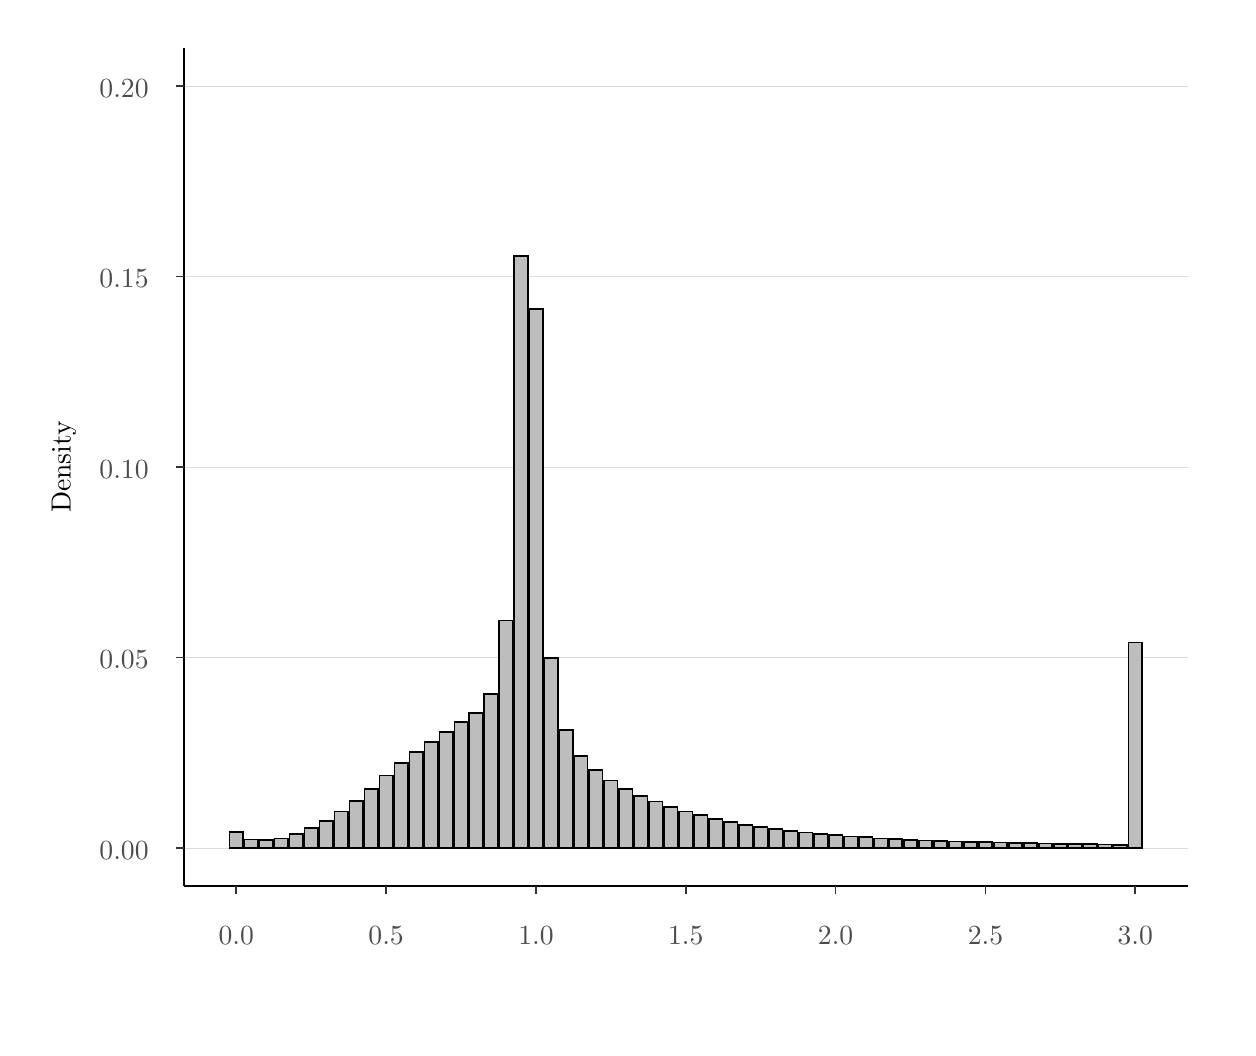
\begin{tikzpicture}[x=1pt,y=1pt]
\definecolor{fillColor}{RGB}{255,255,255}
\path[use as bounding box,fill=fillColor,fill opacity=0.00] (0,0) rectangle (433.62,361.35);
\begin{scope}
\path[clip] (  0.00,  0.00) rectangle (433.62,361.35);
\definecolor{drawColor}{RGB}{255,255,255}
\definecolor{fillColor}{RGB}{255,255,255}

\path[draw=drawColor,line width= 0.6pt,line join=round,line cap=round,fill=fillColor] ( -0.00,  0.00) rectangle (433.62,361.35);
\end{scope}
\begin{scope}
\path[clip] ( 56.47, 51.15) rectangle (419.17,354.12);
\definecolor{drawColor}{RGB}{255,255,255}

\path[draw=drawColor,line width= 0.3pt,line join=round] ( 56.47, 99.35) --
	(419.17, 99.35);

\path[draw=drawColor,line width= 0.3pt,line join=round] ( 56.47,168.21) --
	(419.17,168.21);

\path[draw=drawColor,line width= 0.3pt,line join=round] ( 56.47,237.07) --
	(419.17,237.07);

\path[draw=drawColor,line width= 0.3pt,line join=round] ( 56.47,305.92) --
	(419.17,305.92);

\path[draw=drawColor,line width= 0.3pt,line join=round] (102.46, 51.15) --
	(102.46,354.12);

\path[draw=drawColor,line width= 0.3pt,line join=round] (156.60, 51.15) --
	(156.60,354.12);

\path[draw=drawColor,line width= 0.3pt,line join=round] (210.74, 51.15) --
	(210.74,354.12);

\path[draw=drawColor,line width= 0.3pt,line join=round] (264.89, 51.15) --
	(264.89,354.12);

\path[draw=drawColor,line width= 0.3pt,line join=round] (319.03, 51.15) --
	(319.03,354.12);

\path[draw=drawColor,line width= 0.3pt,line join=round] (373.17, 51.15) --
	(373.17,354.12);
\definecolor{drawColor}{gray}{0.85}

\path[draw=drawColor,line width= 0.1pt,line join=round] ( 56.47, 64.92) --
	(419.17, 64.92);

\path[draw=drawColor,line width= 0.1pt,line join=round] ( 56.47,133.78) --
	(419.17,133.78);

\path[draw=drawColor,line width= 0.1pt,line join=round] ( 56.47,202.64) --
	(419.17,202.64);

\path[draw=drawColor,line width= 0.1pt,line join=round] ( 56.47,271.49) --
	(419.17,271.49);

\path[draw=drawColor,line width= 0.1pt,line join=round] ( 56.47,340.35) --
	(419.17,340.35);
\definecolor{drawColor}{RGB}{0,0,0}
\definecolor{fillColor}{gray}{0.74}

\path[draw=drawColor,line width= 0.6pt,line cap=rect,fill=fillColor] ( 72.95, 64.92) rectangle ( 77.82, 70.68);

\path[draw=drawColor,line width= 0.6pt,line cap=rect,fill=fillColor] ( 78.37, 64.92) rectangle ( 83.24, 67.96);

\path[draw=drawColor,line width= 0.6pt,line cap=rect,fill=fillColor] ( 83.78, 64.92) rectangle ( 88.65, 67.82);

\path[draw=drawColor,line width= 0.6pt,line cap=rect,fill=fillColor] ( 89.19, 64.92) rectangle ( 94.07, 68.39);

\path[draw=drawColor,line width= 0.6pt,line cap=rect,fill=fillColor] ( 94.61, 64.92) rectangle ( 99.48, 69.89);

\path[draw=drawColor,line width= 0.6pt,line cap=rect,fill=fillColor] (100.02, 64.92) rectangle (104.90, 72.04);

\path[draw=drawColor,line width= 0.6pt,line cap=rect,fill=fillColor] (105.44, 64.92) rectangle (110.31, 74.73);

\path[draw=drawColor,line width= 0.6pt,line cap=rect,fill=fillColor] (110.85, 64.92) rectangle (115.72, 78.10);

\path[draw=drawColor,line width= 0.6pt,line cap=rect,fill=fillColor] (116.27, 64.92) rectangle (121.14, 81.79);

\path[draw=drawColor,line width= 0.6pt,line cap=rect,fill=fillColor] (121.68, 64.92) rectangle (126.55, 86.29);

\path[draw=drawColor,line width= 0.6pt,line cap=rect,fill=fillColor] (127.09, 64.92) rectangle (131.97, 91.12);

\path[draw=drawColor,line width= 0.6pt,line cap=rect,fill=fillColor] (132.51, 64.92) rectangle (137.38, 95.52);

\path[draw=drawColor,line width= 0.6pt,line cap=rect,fill=fillColor] (137.92, 64.92) rectangle (142.80, 99.56);

\path[draw=drawColor,line width= 0.6pt,line cap=rect,fill=fillColor] (143.34, 64.92) rectangle (148.21,103.34);

\path[draw=drawColor,line width= 0.6pt,line cap=rect,fill=fillColor] (148.75, 64.92) rectangle (153.62,106.76);

\path[draw=drawColor,line width= 0.6pt,line cap=rect,fill=fillColor] (154.17, 64.92) rectangle (159.04,110.44);

\path[draw=drawColor,line width= 0.6pt,line cap=rect,fill=fillColor] (159.58, 64.92) rectangle (164.45,113.75);

\path[draw=drawColor,line width= 0.6pt,line cap=rect,fill=fillColor] (164.99, 64.92) rectangle (169.87,120.67);

\path[draw=drawColor,line width= 0.6pt,line cap=rect,fill=fillColor] (170.41, 64.92) rectangle (175.28,147.18);

\path[draw=drawColor,line width= 0.6pt,line cap=rect,fill=fillColor] (175.82, 64.92) rectangle (180.70,278.85);

\path[draw=drawColor,line width= 0.6pt,line cap=rect,fill=fillColor] (181.24, 64.92) rectangle (186.11,259.61);

\path[draw=drawColor,line width= 0.6pt,line cap=rect,fill=fillColor] (186.65, 64.92) rectangle (191.52,133.47);

\path[draw=drawColor,line width= 0.6pt,line cap=rect,fill=fillColor] (192.07, 64.92) rectangle (196.94,107.53);

\path[draw=drawColor,line width= 0.6pt,line cap=rect,fill=fillColor] (197.48, 64.92) rectangle (202.35, 98.23);

\path[draw=drawColor,line width= 0.6pt,line cap=rect,fill=fillColor] (202.89, 64.92) rectangle (207.77, 93.16);

\path[draw=drawColor,line width= 0.6pt,line cap=rect,fill=fillColor] (208.31, 64.92) rectangle (213.18, 89.35);

\path[draw=drawColor,line width= 0.6pt,line cap=rect,fill=fillColor] (213.72, 64.92) rectangle (218.60, 86.27);

\path[draw=drawColor,line width= 0.6pt,line cap=rect,fill=fillColor] (219.14, 64.92) rectangle (224.01, 83.82);

\path[draw=drawColor,line width= 0.6pt,line cap=rect,fill=fillColor] (224.55, 64.92) rectangle (229.42, 81.72);

\path[draw=drawColor,line width= 0.6pt,line cap=rect,fill=fillColor] (229.97, 64.92) rectangle (234.84, 79.80);

\path[draw=drawColor,line width= 0.6pt,line cap=rect,fill=fillColor] (235.38, 64.92) rectangle (240.25, 78.17);

\path[draw=drawColor,line width= 0.6pt,line cap=rect,fill=fillColor] (240.79, 64.92) rectangle (245.67, 76.75);

\path[draw=drawColor,line width= 0.6pt,line cap=rect,fill=fillColor] (246.21, 64.92) rectangle (251.08, 75.32);

\path[draw=drawColor,line width= 0.6pt,line cap=rect,fill=fillColor] (251.62, 64.92) rectangle (256.50, 74.25);

\path[draw=drawColor,line width= 0.6pt,line cap=rect,fill=fillColor] (257.04, 64.92) rectangle (261.91, 73.33);

\path[draw=drawColor,line width= 0.6pt,line cap=rect,fill=fillColor] (262.45, 64.92) rectangle (267.32, 72.52);

\path[draw=drawColor,line width= 0.6pt,line cap=rect,fill=fillColor] (267.86, 64.92) rectangle (272.74, 71.84);

\path[draw=drawColor,line width= 0.6pt,line cap=rect,fill=fillColor] (273.28, 64.92) rectangle (278.15, 71.14);

\path[draw=drawColor,line width= 0.6pt,line cap=rect,fill=fillColor] (278.69, 64.92) rectangle (283.57, 70.47);

\path[draw=drawColor,line width= 0.6pt,line cap=rect,fill=fillColor] (284.11, 64.92) rectangle (288.98, 69.99);

\path[draw=drawColor,line width= 0.6pt,line cap=rect,fill=fillColor] (289.52, 64.92) rectangle (294.39, 69.64);

\path[draw=drawColor,line width= 0.6pt,line cap=rect,fill=fillColor] (294.94, 64.92) rectangle (299.81, 69.14);

\path[draw=drawColor,line width= 0.6pt,line cap=rect,fill=fillColor] (300.35, 64.92) rectangle (305.22, 68.83);

\path[draw=drawColor,line width= 0.6pt,line cap=rect,fill=fillColor] (305.76, 64.92) rectangle (310.64, 68.38);

\path[draw=drawColor,line width= 0.6pt,line cap=rect,fill=fillColor] (311.18, 64.92) rectangle (316.05, 68.15);

\path[draw=drawColor,line width= 0.6pt,line cap=rect,fill=fillColor] (316.59, 64.92) rectangle (321.47, 67.93);

\path[draw=drawColor,line width= 0.6pt,line cap=rect,fill=fillColor] (322.01, 64.92) rectangle (326.88, 67.69);

\path[draw=drawColor,line width= 0.6pt,line cap=rect,fill=fillColor] (327.42, 64.92) rectangle (332.29, 67.48);

\path[draw=drawColor,line width= 0.6pt,line cap=rect,fill=fillColor] (332.84, 64.92) rectangle (337.71, 67.30);

\path[draw=drawColor,line width= 0.6pt,line cap=rect,fill=fillColor] (338.25, 64.92) rectangle (343.12, 67.08);

\path[draw=drawColor,line width= 0.6pt,line cap=rect,fill=fillColor] (343.66, 64.92) rectangle (348.54, 67.04);

\path[draw=drawColor,line width= 0.6pt,line cap=rect,fill=fillColor] (349.08, 64.92) rectangle (353.95, 66.87);

\path[draw=drawColor,line width= 0.6pt,line cap=rect,fill=fillColor] (354.49, 64.92) rectangle (359.37, 66.68);

\path[draw=drawColor,line width= 0.6pt,line cap=rect,fill=fillColor] (359.91, 64.92) rectangle (364.78, 66.64);

\path[draw=drawColor,line width= 0.6pt,line cap=rect,fill=fillColor] (365.32, 64.92) rectangle (370.19, 66.52);

\path[draw=drawColor,line width= 0.6pt,line cap=rect,fill=fillColor] (370.74, 64.92) rectangle (375.61, 66.45);

\path[draw=drawColor,line width= 0.6pt,line cap=rect,fill=fillColor] (376.15, 64.92) rectangle (381.02, 66.34);

\path[draw=drawColor,line width= 0.6pt,line cap=rect,fill=fillColor] (381.56, 64.92) rectangle (386.44, 66.25);

\path[draw=drawColor,line width= 0.6pt,line cap=rect,fill=fillColor] (386.98, 64.92) rectangle (391.85, 66.22);

\path[draw=drawColor,line width= 0.6pt,line cap=rect,fill=fillColor] (392.39, 64.92) rectangle (397.27, 66.07);

\path[draw=drawColor,line width= 0.6pt,line cap=rect,fill=fillColor] (397.81, 64.92) rectangle (402.68,139.23);
\end{scope}
\begin{scope}
\path[clip] (  0.00,  0.00) rectangle (433.62,361.35);
\definecolor{drawColor}{RGB}{0,0,0}

\path[draw=drawColor,line width= 0.6pt,line join=round] ( 56.47, 51.15) --
	( 56.47,354.12);
\end{scope}
\begin{scope}
\path[clip] (  0.00,  0.00) rectangle (433.62,361.35);
\definecolor{drawColor}{gray}{0.30}

\node[text=drawColor,anchor=base east,inner sep=0pt, outer sep=0pt, scale=  1.00] at ( 43.72, 60.79) {0.00};

\node[text=drawColor,anchor=base east,inner sep=0pt, outer sep=0pt, scale=  1.00] at ( 43.72,129.65) {0.05};

\node[text=drawColor,anchor=base east,inner sep=0pt, outer sep=0pt, scale=  1.00] at ( 43.72,198.51) {0.10};

\node[text=drawColor,anchor=base east,inner sep=0pt, outer sep=0pt, scale=  1.00] at ( 43.72,267.36) {0.15};

\node[text=drawColor,anchor=base east,inner sep=0pt, outer sep=0pt, scale=  1.00] at ( 43.72,336.22) {0.20};
\end{scope}
\begin{scope}
\path[clip] (  0.00,  0.00) rectangle (433.62,361.35);
\definecolor{drawColor}{gray}{0.20}

\path[draw=drawColor,line width= 0.6pt,line join=round] ( 53.72, 64.92) --
	( 56.47, 64.92);

\path[draw=drawColor,line width= 0.6pt,line join=round] ( 53.72,133.78) --
	( 56.47,133.78);

\path[draw=drawColor,line width= 0.6pt,line join=round] ( 53.72,202.64) --
	( 56.47,202.64);

\path[draw=drawColor,line width= 0.6pt,line join=round] ( 53.72,271.49) --
	( 56.47,271.49);

\path[draw=drawColor,line width= 0.6pt,line join=round] ( 53.72,340.35) --
	( 56.47,340.35);
\end{scope}
\begin{scope}
\path[clip] (  0.00,  0.00) rectangle (433.62,361.35);
\definecolor{drawColor}{RGB}{0,0,0}

\path[draw=drawColor,line width= 0.6pt,line join=round] ( 56.47, 51.15) --
	(419.17, 51.15);
\end{scope}
\begin{scope}
\path[clip] (  0.00,  0.00) rectangle (433.62,361.35);
\definecolor{drawColor}{gray}{0.20}

\path[draw=drawColor,line width= 0.6pt,line join=round] ( 75.39, 48.40) --
	( 75.39, 51.15);

\path[draw=drawColor,line width= 0.6pt,line join=round] (129.53, 48.40) --
	(129.53, 51.15);

\path[draw=drawColor,line width= 0.6pt,line join=round] (183.67, 48.40) --
	(183.67, 51.15);

\path[draw=drawColor,line width= 0.6pt,line join=round] (237.82, 48.40) --
	(237.82, 51.15);

\path[draw=drawColor,line width= 0.6pt,line join=round] (291.96, 48.40) --
	(291.96, 51.15);

\path[draw=drawColor,line width= 0.6pt,line join=round] (346.10, 48.40) --
	(346.10, 51.15);

\path[draw=drawColor,line width= 0.6pt,line join=round] (400.24, 48.40) --
	(400.24, 51.15);
\end{scope}
\begin{scope}
\path[clip] (  0.00,  0.00) rectangle (433.62,361.35);
\definecolor{drawColor}{gray}{0.30}

\node[text=drawColor,anchor=base,inner sep=0pt, outer sep=0pt, scale=  1.00] at ( 75.39, 30.14) {0.0};

\node[text=drawColor,anchor=base,inner sep=0pt, outer sep=0pt, scale=  1.00] at (129.53, 30.14) {0.5};

\node[text=drawColor,anchor=base,inner sep=0pt, outer sep=0pt, scale=  1.00] at (183.67, 30.14) {1.0};

\node[text=drawColor,anchor=base,inner sep=0pt, outer sep=0pt, scale=  1.00] at (237.82, 30.14) {1.5};

\node[text=drawColor,anchor=base,inner sep=0pt, outer sep=0pt, scale=  1.00] at (291.96, 30.14) {2.0};

\node[text=drawColor,anchor=base,inner sep=0pt, outer sep=0pt, scale=  1.00] at (346.10, 30.14) {2.5};

\node[text=drawColor,anchor=base,inner sep=0pt, outer sep=0pt, scale=  1.00] at (400.24, 30.14) {3.0};
\end{scope}
\begin{scope}
\path[clip] (  0.00,  0.00) rectangle (433.62,361.35);
\definecolor{drawColor}{RGB}{0,0,0}

\node[text=drawColor,rotate= 90.00,anchor=base,inner sep=0pt, outer sep=0pt, scale=  1.00] at ( 15.49,202.64) {Density};
\end{scope}
\end{tikzpicture}
}
     \end{subfigure}
     \begin{subfigure}[t]{.49\textwidth}
         \centering
         \caption{$\lambda^{F,ll'}_{pl',t}\bigg/\lambda^{F,ll'}_{pl,t}$}
         \label{fig: feenstra_firm}
         \scalebox{0.45}{% Created by tikzDevice version 0.12.3.1 on 2022-10-27 20:08:00
% !TEX encoding = UTF-8 Unicode
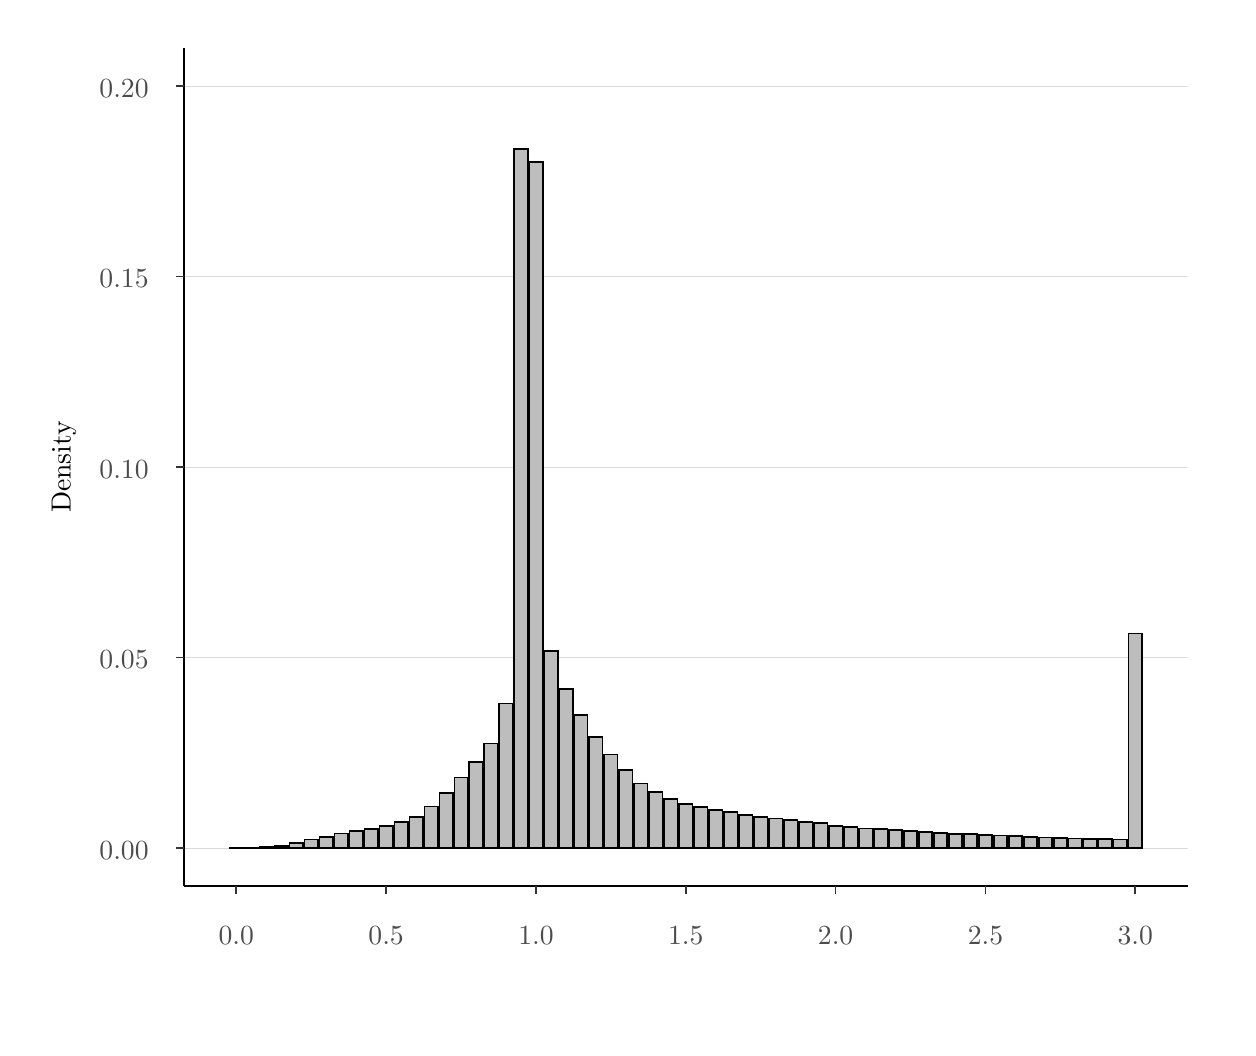
\begin{tikzpicture}[x=1pt,y=1pt]
\definecolor{fillColor}{RGB}{255,255,255}
\path[use as bounding box,fill=fillColor,fill opacity=0.00] (0,0) rectangle (433.62,361.35);
\begin{scope}
\path[clip] (  0.00,  0.00) rectangle (433.62,361.35);
\definecolor{drawColor}{RGB}{255,255,255}
\definecolor{fillColor}{RGB}{255,255,255}

\path[draw=drawColor,line width= 0.6pt,line join=round,line cap=round,fill=fillColor] ( -0.00,  0.00) rectangle (433.62,361.35);
\end{scope}
\begin{scope}
\path[clip] ( 56.47, 51.15) rectangle (419.17,354.12);
\definecolor{drawColor}{RGB}{255,255,255}

\path[draw=drawColor,line width= 0.3pt,line join=round] ( 56.47, 99.35) --
	(419.17, 99.35);

\path[draw=drawColor,line width= 0.3pt,line join=round] ( 56.47,168.21) --
	(419.17,168.21);

\path[draw=drawColor,line width= 0.3pt,line join=round] ( 56.47,237.07) --
	(419.17,237.07);

\path[draw=drawColor,line width= 0.3pt,line join=round] ( 56.47,305.92) --
	(419.17,305.92);

\path[draw=drawColor,line width= 0.3pt,line join=round] (102.46, 51.15) --
	(102.46,354.12);

\path[draw=drawColor,line width= 0.3pt,line join=round] (156.60, 51.15) --
	(156.60,354.12);

\path[draw=drawColor,line width= 0.3pt,line join=round] (210.74, 51.15) --
	(210.74,354.12);

\path[draw=drawColor,line width= 0.3pt,line join=round] (264.89, 51.15) --
	(264.89,354.12);

\path[draw=drawColor,line width= 0.3pt,line join=round] (319.03, 51.15) --
	(319.03,354.12);

\path[draw=drawColor,line width= 0.3pt,line join=round] (373.17, 51.15) --
	(373.17,354.12);
\definecolor{drawColor}{gray}{0.85}

\path[draw=drawColor,line width= 0.1pt,line join=round] ( 56.47, 64.92) --
	(419.17, 64.92);

\path[draw=drawColor,line width= 0.1pt,line join=round] ( 56.47,133.78) --
	(419.17,133.78);

\path[draw=drawColor,line width= 0.1pt,line join=round] ( 56.47,202.64) --
	(419.17,202.64);

\path[draw=drawColor,line width= 0.1pt,line join=round] ( 56.47,271.49) --
	(419.17,271.49);

\path[draw=drawColor,line width= 0.1pt,line join=round] ( 56.47,340.35) --
	(419.17,340.35);
\definecolor{drawColor}{RGB}{0,0,0}
\definecolor{fillColor}{gray}{0.74}

\path[draw=drawColor,line width= 0.6pt,line cap=rect,fill=fillColor] ( 72.95, 64.92) rectangle ( 77.82, 64.94);

\path[draw=drawColor,line width= 0.6pt,line cap=rect,fill=fillColor] ( 78.37, 64.92) rectangle ( 83.24, 65.00);

\path[draw=drawColor,line width= 0.6pt,line cap=rect,fill=fillColor] ( 83.78, 64.92) rectangle ( 88.65, 65.26);

\path[draw=drawColor,line width= 0.6pt,line cap=rect,fill=fillColor] ( 89.19, 64.92) rectangle ( 94.07, 65.71);

\path[draw=drawColor,line width= 0.6pt,line cap=rect,fill=fillColor] ( 94.61, 64.92) rectangle ( 99.48, 66.63);

\path[draw=drawColor,line width= 0.6pt,line cap=rect,fill=fillColor] (100.02, 64.92) rectangle (104.90, 67.94);

\path[draw=drawColor,line width= 0.6pt,line cap=rect,fill=fillColor] (105.44, 64.92) rectangle (110.31, 68.98);

\path[draw=drawColor,line width= 0.6pt,line cap=rect,fill=fillColor] (110.85, 64.92) rectangle (115.72, 70.17);

\path[draw=drawColor,line width= 0.6pt,line cap=rect,fill=fillColor] (116.27, 64.92) rectangle (121.14, 71.12);

\path[draw=drawColor,line width= 0.6pt,line cap=rect,fill=fillColor] (121.68, 64.92) rectangle (126.55, 71.87);

\path[draw=drawColor,line width= 0.6pt,line cap=rect,fill=fillColor] (127.09, 64.92) rectangle (131.97, 72.89);

\path[draw=drawColor,line width= 0.6pt,line cap=rect,fill=fillColor] (132.51, 64.92) rectangle (137.38, 74.24);

\path[draw=drawColor,line width= 0.6pt,line cap=rect,fill=fillColor] (137.92, 64.92) rectangle (142.80, 76.14);

\path[draw=drawColor,line width= 0.6pt,line cap=rect,fill=fillColor] (143.34, 64.92) rectangle (148.21, 79.93);

\path[draw=drawColor,line width= 0.6pt,line cap=rect,fill=fillColor] (148.75, 64.92) rectangle (153.62, 84.72);

\path[draw=drawColor,line width= 0.6pt,line cap=rect,fill=fillColor] (154.17, 64.92) rectangle (159.04, 90.44);

\path[draw=drawColor,line width= 0.6pt,line cap=rect,fill=fillColor] (159.58, 64.92) rectangle (164.45, 95.89);

\path[draw=drawColor,line width= 0.6pt,line cap=rect,fill=fillColor] (164.99, 64.92) rectangle (169.87,102.72);

\path[draw=drawColor,line width= 0.6pt,line cap=rect,fill=fillColor] (170.41, 64.92) rectangle (175.28,117.17);

\path[draw=drawColor,line width= 0.6pt,line cap=rect,fill=fillColor] (175.82, 64.92) rectangle (180.70,317.45);

\path[draw=drawColor,line width= 0.6pt,line cap=rect,fill=fillColor] (181.24, 64.92) rectangle (186.11,312.75);

\path[draw=drawColor,line width= 0.6pt,line cap=rect,fill=fillColor] (186.65, 64.92) rectangle (191.52,136.13);

\path[draw=drawColor,line width= 0.6pt,line cap=rect,fill=fillColor] (192.07, 64.92) rectangle (196.94,122.41);

\path[draw=drawColor,line width= 0.6pt,line cap=rect,fill=fillColor] (197.48, 64.92) rectangle (202.35,112.94);

\path[draw=drawColor,line width= 0.6pt,line cap=rect,fill=fillColor] (202.89, 64.92) rectangle (207.77,104.98);

\path[draw=drawColor,line width= 0.6pt,line cap=rect,fill=fillColor] (208.31, 64.92) rectangle (213.18, 98.69);

\path[draw=drawColor,line width= 0.6pt,line cap=rect,fill=fillColor] (213.72, 64.92) rectangle (218.60, 93.13);

\path[draw=drawColor,line width= 0.6pt,line cap=rect,fill=fillColor] (219.14, 64.92) rectangle (224.01, 88.27);

\path[draw=drawColor,line width= 0.6pt,line cap=rect,fill=fillColor] (224.55, 64.92) rectangle (229.42, 85.09);

\path[draw=drawColor,line width= 0.6pt,line cap=rect,fill=fillColor] (229.97, 64.92) rectangle (234.84, 82.70);

\path[draw=drawColor,line width= 0.6pt,line cap=rect,fill=fillColor] (235.38, 64.92) rectangle (240.25, 80.88);

\path[draw=drawColor,line width= 0.6pt,line cap=rect,fill=fillColor] (240.79, 64.92) rectangle (245.67, 79.65);

\path[draw=drawColor,line width= 0.6pt,line cap=rect,fill=fillColor] (246.21, 64.92) rectangle (251.08, 78.69);

\path[draw=drawColor,line width= 0.6pt,line cap=rect,fill=fillColor] (251.62, 64.92) rectangle (256.50, 77.85);

\path[draw=drawColor,line width= 0.6pt,line cap=rect,fill=fillColor] (257.04, 64.92) rectangle (261.91, 76.93);

\path[draw=drawColor,line width= 0.6pt,line cap=rect,fill=fillColor] (262.45, 64.92) rectangle (267.32, 76.20);

\path[draw=drawColor,line width= 0.6pt,line cap=rect,fill=fillColor] (267.86, 64.92) rectangle (272.74, 75.63);

\path[draw=drawColor,line width= 0.6pt,line cap=rect,fill=fillColor] (273.28, 64.92) rectangle (278.15, 74.97);

\path[draw=drawColor,line width= 0.6pt,line cap=rect,fill=fillColor] (278.69, 64.92) rectangle (283.57, 74.25);

\path[draw=drawColor,line width= 0.6pt,line cap=rect,fill=fillColor] (284.11, 64.92) rectangle (288.98, 73.84);

\path[draw=drawColor,line width= 0.6pt,line cap=rect,fill=fillColor] (289.52, 64.92) rectangle (294.39, 72.99);

\path[draw=drawColor,line width= 0.6pt,line cap=rect,fill=fillColor] (294.94, 64.92) rectangle (299.81, 72.48);

\path[draw=drawColor,line width= 0.6pt,line cap=rect,fill=fillColor] (300.35, 64.92) rectangle (305.22, 71.95);

\path[draw=drawColor,line width= 0.6pt,line cap=rect,fill=fillColor] (305.76, 64.92) rectangle (310.64, 71.67);

\path[draw=drawColor,line width= 0.6pt,line cap=rect,fill=fillColor] (311.18, 64.92) rectangle (316.05, 71.38);

\path[draw=drawColor,line width= 0.6pt,line cap=rect,fill=fillColor] (316.59, 64.92) rectangle (321.47, 71.00);

\path[draw=drawColor,line width= 0.6pt,line cap=rect,fill=fillColor] (322.01, 64.92) rectangle (326.88, 70.68);

\path[draw=drawColor,line width= 0.6pt,line cap=rect,fill=fillColor] (327.42, 64.92) rectangle (332.29, 70.44);

\path[draw=drawColor,line width= 0.6pt,line cap=rect,fill=fillColor] (332.84, 64.92) rectangle (337.71, 70.00);

\path[draw=drawColor,line width= 0.6pt,line cap=rect,fill=fillColor] (338.25, 64.92) rectangle (343.12, 69.91);

\path[draw=drawColor,line width= 0.6pt,line cap=rect,fill=fillColor] (343.66, 64.92) rectangle (348.54, 69.62);

\path[draw=drawColor,line width= 0.6pt,line cap=rect,fill=fillColor] (349.08, 64.92) rectangle (353.95, 69.43);

\path[draw=drawColor,line width= 0.6pt,line cap=rect,fill=fillColor] (354.49, 64.92) rectangle (359.37, 69.16);

\path[draw=drawColor,line width= 0.6pt,line cap=rect,fill=fillColor] (359.91, 64.92) rectangle (364.78, 68.98);

\path[draw=drawColor,line width= 0.6pt,line cap=rect,fill=fillColor] (365.32, 64.92) rectangle (370.19, 68.75);

\path[draw=drawColor,line width= 0.6pt,line cap=rect,fill=fillColor] (370.74, 64.92) rectangle (375.61, 68.55);

\path[draw=drawColor,line width= 0.6pt,line cap=rect,fill=fillColor] (376.15, 64.92) rectangle (381.02, 68.41);

\path[draw=drawColor,line width= 0.6pt,line cap=rect,fill=fillColor] (381.56, 64.92) rectangle (386.44, 68.25);

\path[draw=drawColor,line width= 0.6pt,line cap=rect,fill=fillColor] (386.98, 64.92) rectangle (391.85, 68.24);

\path[draw=drawColor,line width= 0.6pt,line cap=rect,fill=fillColor] (392.39, 64.92) rectangle (397.27, 68.00);

\path[draw=drawColor,line width= 0.6pt,line cap=rect,fill=fillColor] (397.81, 64.92) rectangle (402.68,142.43);
\end{scope}
\begin{scope}
\path[clip] (  0.00,  0.00) rectangle (433.62,361.35);
\definecolor{drawColor}{RGB}{0,0,0}

\path[draw=drawColor,line width= 0.6pt,line join=round] ( 56.47, 51.15) --
	( 56.47,354.12);
\end{scope}
\begin{scope}
\path[clip] (  0.00,  0.00) rectangle (433.62,361.35);
\definecolor{drawColor}{gray}{0.30}

\node[text=drawColor,anchor=base east,inner sep=0pt, outer sep=0pt, scale=  1.00] at ( 43.72, 60.79) {0.00};

\node[text=drawColor,anchor=base east,inner sep=0pt, outer sep=0pt, scale=  1.00] at ( 43.72,129.65) {0.05};

\node[text=drawColor,anchor=base east,inner sep=0pt, outer sep=0pt, scale=  1.00] at ( 43.72,198.51) {0.10};

\node[text=drawColor,anchor=base east,inner sep=0pt, outer sep=0pt, scale=  1.00] at ( 43.72,267.36) {0.15};

\node[text=drawColor,anchor=base east,inner sep=0pt, outer sep=0pt, scale=  1.00] at ( 43.72,336.22) {0.20};
\end{scope}
\begin{scope}
\path[clip] (  0.00,  0.00) rectangle (433.62,361.35);
\definecolor{drawColor}{gray}{0.20}

\path[draw=drawColor,line width= 0.6pt,line join=round] ( 53.72, 64.92) --
	( 56.47, 64.92);

\path[draw=drawColor,line width= 0.6pt,line join=round] ( 53.72,133.78) --
	( 56.47,133.78);

\path[draw=drawColor,line width= 0.6pt,line join=round] ( 53.72,202.64) --
	( 56.47,202.64);

\path[draw=drawColor,line width= 0.6pt,line join=round] ( 53.72,271.49) --
	( 56.47,271.49);

\path[draw=drawColor,line width= 0.6pt,line join=round] ( 53.72,340.35) --
	( 56.47,340.35);
\end{scope}
\begin{scope}
\path[clip] (  0.00,  0.00) rectangle (433.62,361.35);
\definecolor{drawColor}{RGB}{0,0,0}

\path[draw=drawColor,line width= 0.6pt,line join=round] ( 56.47, 51.15) --
	(419.17, 51.15);
\end{scope}
\begin{scope}
\path[clip] (  0.00,  0.00) rectangle (433.62,361.35);
\definecolor{drawColor}{gray}{0.20}

\path[draw=drawColor,line width= 0.6pt,line join=round] ( 75.39, 48.40) --
	( 75.39, 51.15);

\path[draw=drawColor,line width= 0.6pt,line join=round] (129.53, 48.40) --
	(129.53, 51.15);

\path[draw=drawColor,line width= 0.6pt,line join=round] (183.67, 48.40) --
	(183.67, 51.15);

\path[draw=drawColor,line width= 0.6pt,line join=round] (237.82, 48.40) --
	(237.82, 51.15);

\path[draw=drawColor,line width= 0.6pt,line join=round] (291.96, 48.40) --
	(291.96, 51.15);

\path[draw=drawColor,line width= 0.6pt,line join=round] (346.10, 48.40) --
	(346.10, 51.15);

\path[draw=drawColor,line width= 0.6pt,line join=round] (400.24, 48.40) --
	(400.24, 51.15);
\end{scope}
\begin{scope}
\path[clip] (  0.00,  0.00) rectangle (433.62,361.35);
\definecolor{drawColor}{gray}{0.30}

\node[text=drawColor,anchor=base,inner sep=0pt, outer sep=0pt, scale=  1.00] at ( 75.39, 30.14) {0.0};

\node[text=drawColor,anchor=base,inner sep=0pt, outer sep=0pt, scale=  1.00] at (129.53, 30.14) {0.5};

\node[text=drawColor,anchor=base,inner sep=0pt, outer sep=0pt, scale=  1.00] at (183.67, 30.14) {1.0};

\node[text=drawColor,anchor=base,inner sep=0pt, outer sep=0pt, scale=  1.00] at (237.82, 30.14) {1.5};

\node[text=drawColor,anchor=base,inner sep=0pt, outer sep=0pt, scale=  1.00] at (291.96, 30.14) {2.0};

\node[text=drawColor,anchor=base,inner sep=0pt, outer sep=0pt, scale=  1.00] at (346.10, 30.14) {2.5};

\node[text=drawColor,anchor=base,inner sep=0pt, outer sep=0pt, scale=  1.00] at (400.24, 30.14) {3.0};
\end{scope}
\begin{scope}
\path[clip] (  0.00,  0.00) rectangle (433.62,361.35);
\definecolor{drawColor}{RGB}{0,0,0}

\node[text=drawColor,rotate= 90.00,anchor=base,inner sep=0pt, outer sep=0pt, scale=  1.00] at ( 15.49,202.64) {Density};
\end{scope}
\end{tikzpicture}
}
     \end{subfigure}
     \parbox{\textwidth}{
        \begin{spacing}{1} 
            {\footnotesize 
            \textit{Notes}: This figure plots the distribution for the relative expenditure share on common product varieties and common firms in panel (a) and panel (b) respectively. The unit of observation is at the product category-region $l$-region $l'$-year level. Within each product category, we compute for each NUTS2-region combination the ratio of expenditure on either common product varieties or common firms relative total expenditure. Hereafter, we bin the data into 0.05 bins and winsorize the data at a relative share of 3.}
        \end{spacing}}
\end{figure} 
